\documentclass{entwurfsheft}

% glossary
\makeglossaries

\begin{document}
\newglossaryentry{label}{
    name=Label,
    plural=Labels,
    description={Rezepte können mit bezeichnenden Stichwörtern, sogenannten Labels, versehen werden. Dies ermöglicht das Filtern von Rezepten nach bestimmten Eigenschaften (z.B. vegetarisch, glutenfrei, halal)}
}
\maketitle
\begin{sloppypar}
\tableofcontents
\newpage

\section*{Gender-Hinweis}
Zur besseren Lesbarkeit wird in diesem Entwurfsheft das generische Maskulinum verwendet.
Die in diesem Heft verwendeten Personenbezeichnungen beziehen sich - sofern nicht anders kenntlich gemacht - auf alle Geschlechter.
\newpage

\section{Allgemeines}
\subsection{Zweck}
Das Entwurfsheft des Projekts: "Write your own Android App: SpiceSquad" baut auf dem zuvor verfassten Pflichtenheft auf.
Hierzu wurde zunächst ein umfassendes Klassendiagramm erstellt. Auf diesem basierend werden alle Klassen, Methoden und Attribute ausführlich erklärt.
In weiteren Kapiteln wird der \glslink{rest}{REST}-Webservice und die Datenbankstruktur beschrieben. Zum besseren Verständnis sind Ablaufbeschreibungen in Form von Sequenzdiagrammen angefügt.

\subsection{Semantik der UML-Diagramme}
Im Folgenden wird eine abgewandelte Version der Standard-UML-Klassendiagramme verwendet. Alle Attribute, einschließlich solcher, die auf andere Klassen verweisen, werden direkt in der Klasse angegeben. Assoziationspfeile stehen lediglich für die "depends on"-Beziehung, was bedeutet, dass eine Klasse eine andere Klasse benötigt oder importieren muss. Die genaue Art der Beziehung zwischen den Klassen wird im begleitenden Text erklärt. Konstruktoren werden in der Form \texttt{Klasse(Parameter parameter): Klasse} angegeben. Im UML-Diagramm können auch Klassen aus der Dart-Sprache, dem Flutter-Framework, aus TypeScript sowie Generics als Typ verwendet werden. Die Notation \texttt{attribut: Klasse?} bedeutet, dass das Attribut einen Null-Typ haben darf. Falls dies nicht explizit angegeben ist, ist dies nicht der Fall.

Wir behalten uns vor weiter private Attribute und Methoden hinzuzufügen, die nicht im Diagramm aufgeführt sind, um die Implementierung zu erleichtern.
\newpage
\section{Struktur}
Im Abschnitt Struktur wird auf die Architektur der Applikation eingegangen.

Hierbei wird zunächst die Client-Server-Architektur beschrieben.
Anschließend wird die Architektur der Android-Applikation erläutert.
Im Anhang befindet sich ein Klassendiagramm, welches die Struktur der Applikation darstellt. 

Ein vollständiges Klassendiagramm des Frontends befindet sich im Anhang (\autoref{fig:classDiagramFrontend}).

\subsection{Client-Server-Architektur}
Wie bereits im Pflichtenheft angeführt, haben wir uns für eine Trennung von Client und Server entschieden, um somit eine höchstmögliche Modularität zu gewährleisten und
Funktionen wie Squads zu ermöglichen. Die Kommunikation erfolgt über REST-Schnittstellen, welche eine einheitliche Schnittstelle mit dem Server bieten und eine einfache Skalierbarkeit ermöglichen.
Im weiteren Verlauf des Entwurfshefts werden die Architekturen von Client und Server näher beschrieben.

Für die Entwicklung der Android-Applikation soll Flutter benutzt werden. Dies bietet einige Vorteile. Flutter ist ein plattformübergreifendes Framework, das es Entwicklern ermöglicht, eine einzige Codebasis zu verwenden, um Apps sowohl für Android als auch für iOS zu erstellen. Dies reduziert den Entwicklungsaufwand erheblich, da Entwickler nicht separate Codes für jede Plattform schreiben müssen. Flutter verwendet die Dart-Programmiersprache, die eine einfache Syntax und eine umfangreiche Bibliothek bietet, um leistungsstarke und ansprechende Benutzeroberflächen zu erstellen. Darüber hinaus verfügt Flutter über eine Hot-Reload-Funktion, die es Entwicklern ermöglicht, Änderungen in Echtzeit zu sehen, was den Entwicklungsprozess beschleunigt. Flutter-Apps sind schnell, reaktionsfähig und bieten eine extrem gute Leistung, da sie direkt auf die nativen Funktionen des Betriebssystems zugreifen. Diese Kombination aus plattformübergreifender Entwicklung, einfacher Sprache, schnellem Entwicklungsprozess und guter Leistung macht Flutter zu einer guten Wahl für die Entwicklung von SpiceSquad.
\newpage
\subsection{Architektur der Android-Applikation}
Die Applikation wird in vier große Schichten gegliedert. Dies dient dazu, die Bestandteile der App nach ihrer Funktion zu gruppieren und die Abhängigkeiten zwischen den einzelnen Komponenten zu minimieren. Dadurch wird die Wartbarkeit massiv verbessert und auch die Erweiterbarkeit der Applikation wird durch diese Strukturierung erleichtert. Die Schichten orientieren sich stark an den Empfehlungen von Google für die Architektur von Android Applikationen. Die vier Schichten sind der \textbf{Presentation Layer}, der \textbf{Application Layer}, der \textbf{Domain Layer} und der \textbf{Data Layer}.
\begin{figure}[htp]
    \centering
    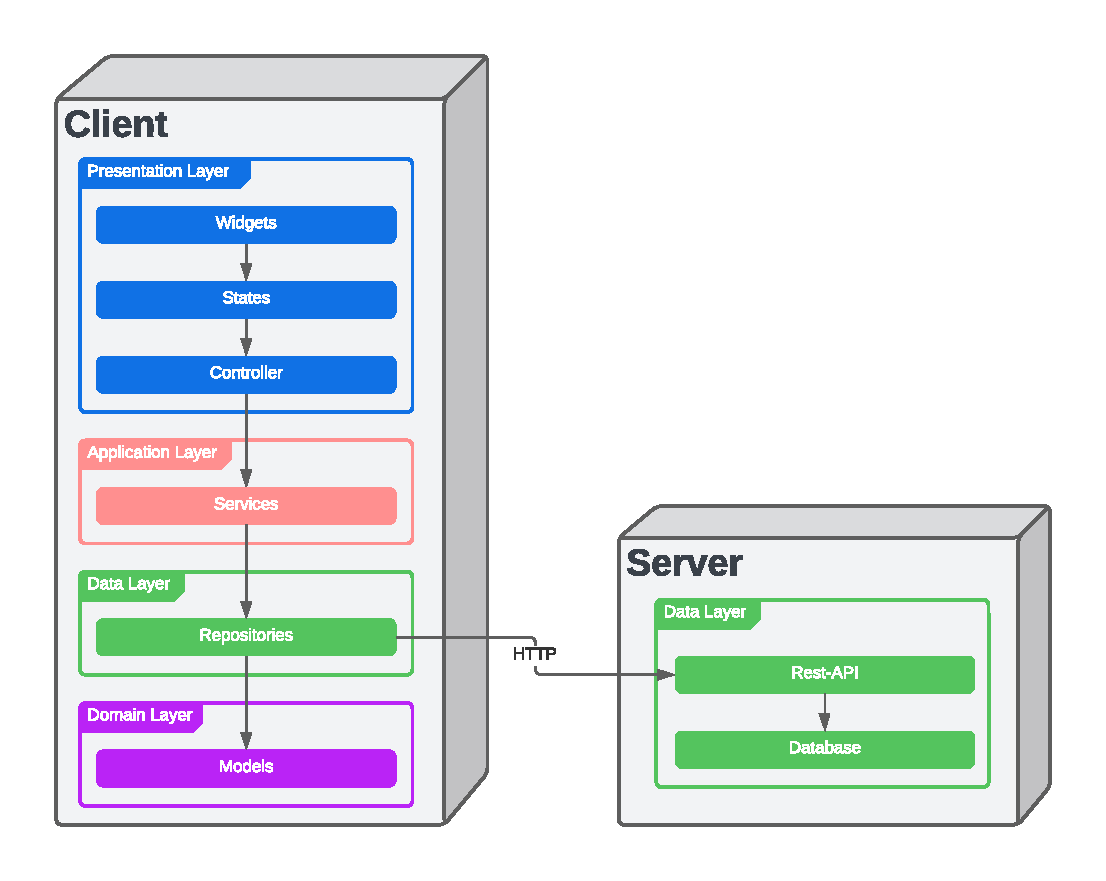
\includegraphics[height = 0.4\textheight]{images/architecture/architecture.pdf}
    \caption{Architektur der Applikation}
    \label{fig:struktur}
\end{figure}

Die Pfeile in der Grafik bedeutet die Richtung der Abhängigkeiten. So kann beispielsweise der Presentation Layer auf den Application Layer zugreifen, aber nicht umgekehrt. Der Presentation Layer dürfte aber auch auf den Data Layer zugreifen. Der Server wird nur von den Repositories über HTTP-Anfragen angesprochen.
Die einzelnen Schichten werden in den folgenden Kapiteln genauer beschrieben.
\newpage

\section{Domain Layer}
Der Domain Layer enthält in erster Linie die Models der einzelnen Entitäten. Diese sollen nun genauer beschrieben werden. In den folgenden Klassendiagrammen wurden Getter der Übersicht halber weggelassen. Sie werden jedoch immer im Text beschrieben, sofern es sie gibt.
\begin{figure}[htp]
    \centering
    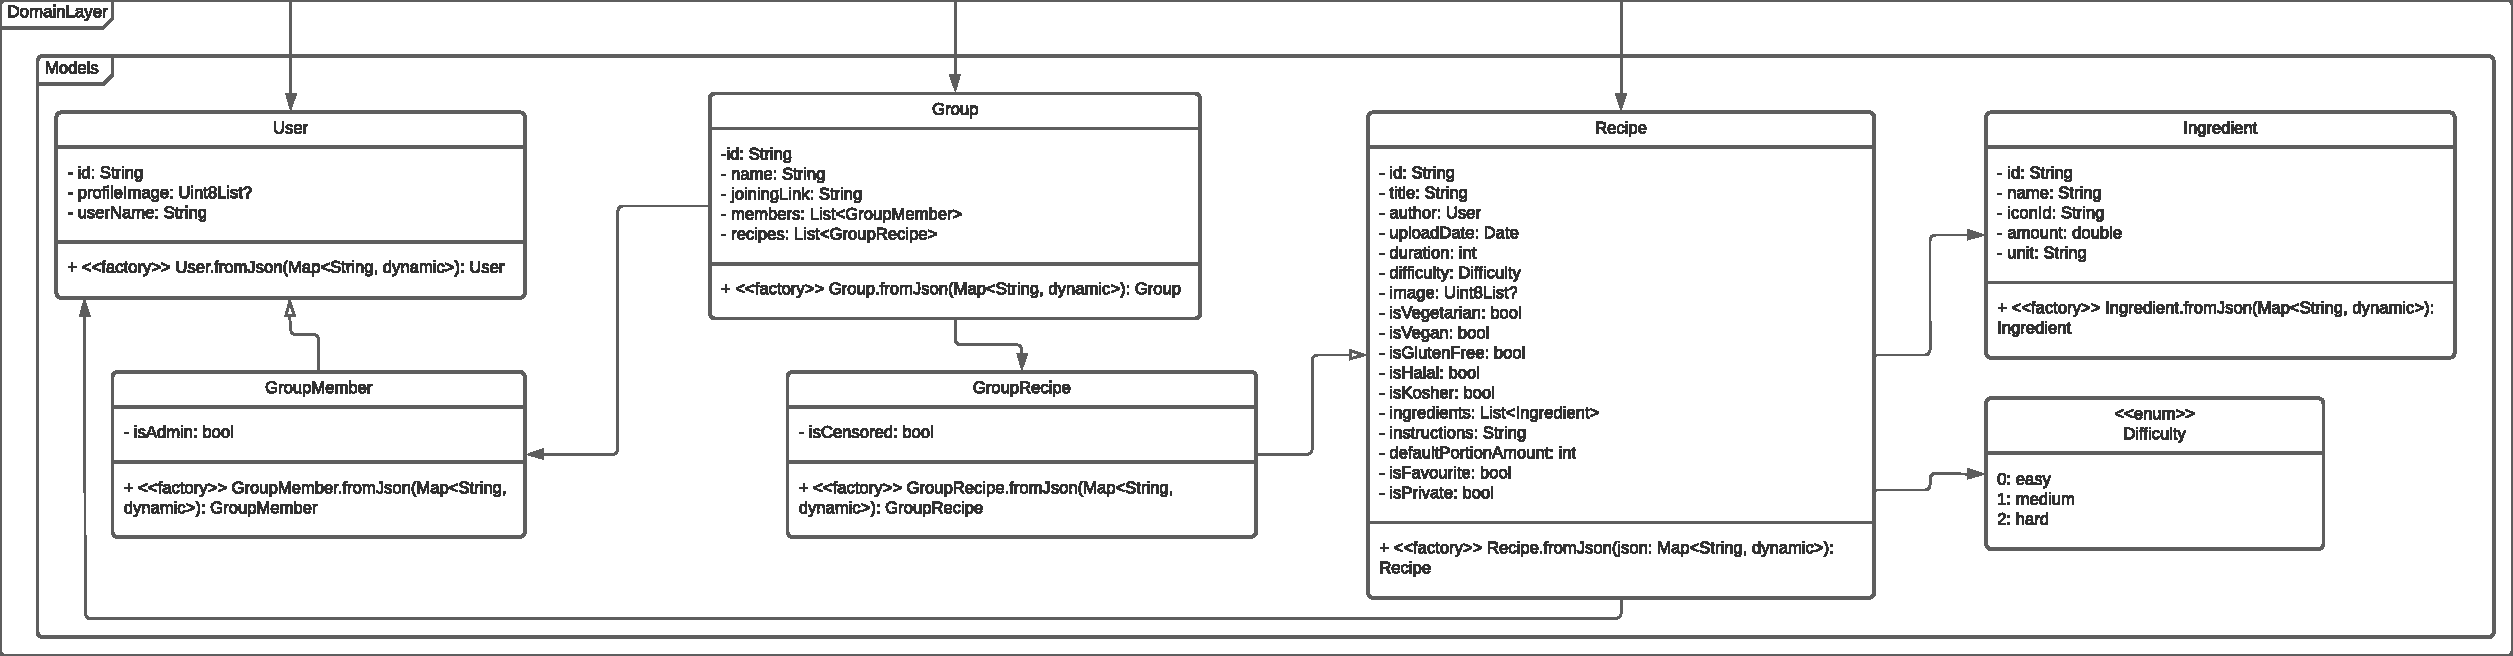
\includegraphics[width = \textwidth]{images/domainLayer/domainLayer.pdf}
    \caption{Klassendiagramm der Model-Klassen}
    \label{fig:domain-layer}
\end{figure}
\newpage
\subsection{\texttt{User}}
\label{sec:user}
Die Klasse \texttt{User} repräsentiert einen Nutzer der App.
\subsubsection*{Attribute}
Alle Attribute sind privat und können nur über einen Getter gelesen werden.
\paragraph{\texttt{id: String}}
Die eindeutige ID des Nutzers. Diese wird vom Server vergeben und ist somit nicht vom Nutzer selbst zu setzen.
\paragraph{\texttt{profileImage: Uint8List?}}
Das Profilbild des Nutzers. Der Typ \texttt{Uint8List} ist ein Array von Bytes, welches das Bild in binärer Form enthält. Dieses Attribut ist optional, da nicht jeder Nutzer ein Profilbild haben muss.
\paragraph{\texttt{username: String}}
Der Nutzername des Nutzers.

\subsubsection*{Methoden}
\paragraph{\texttt{getId(): String}}
Gibt die ID des Nutzers zurück.
\paragraph{\texttt{getProfileImage(): Uint8List?}}
Gibt das Profilbild des Nutzers zurück. Ist kein Profilbild gesetzt, wird null zurückgegeben.
\paragraph{\texttt{getUsername(): String}}
Gibt den Nutzernamen des Nutzers zurück.
\paragraph{\texttt{factory User.fromJson(Map<String, dynamic> json): User}} Factory-Methode, die dazu dient, ein \texttt{User}-Objekt aus einem \glslink{JSON}{JSON-Objekt} zu erstellen. Sie wird verwendet, um die Daten, die vom Server geschickt werden und in \Gls{JSON} vorliegen, in ein \texttt{User}-Objekt umzuwandeln. Die Methode ist statisch, da sie kein \texttt{User}-Objekt benötigt, um aufgerufen zu werden. Nimmt als Parameter das bereits in eine Map umgewandelte \glslink{JSON}{JSON-Objekt} entgegen und gibt ein \texttt{User}-Objekt zurück.
\newpage

\subsection{\texttt{Recipe}}
\label{sec:recipe}
Die Klasse \texttt{Recipe} repräsentiert ein Rezept.
\subsubsection*{Attribute}
Alle Attribute sind privat und können nur über Getter-Methoden abgerufen werden.
\paragraph{\texttt{id: String}}
Die eindeutige ID des Rezepts. Diese wird vom Server vergeben und ist somit nicht vom Nutzer selbst zu setzen.
\paragraph{\texttt{title: String}}
Der Titel des Rezepts.
\paragraph{\texttt{author: User}}
Der Autor des Rezepts.
\paragraph{\texttt{uploadDate: Date}}
Das Datum, an dem das Rezept hochgeladen wurde.
\paragraph{\texttt{duration: int}}
Die Dauer zum Nachkochen des Rezepts in Minuten.
\paragraph{\texttt{difficulty: Difficulty}}
Die \Gls{schwierigkeit} des Rezepts.
\paragraph{\texttt{image: Uint8List?}}
Das Bild des Rezepts. Der Typ Uint8List ist ein Array von Bytes, welches das Bild in binärer Form enthält. Dieses Attribut ist optional, da nicht jedes Rezept ein Bild haben muss.
\paragraph{\texttt{isVegetartian: bool}}
Gibt an, ob das \Gls{label} "Vegetarisch" aktiviert ist.
\paragraph{\texttt{isVegan: bool}}
Gibt an, ob das \Gls{label} "Vegan" aktiviert ist.
\paragraph{\texttt{isGlutenFree: bool}}
Gibt an, ob das \Gls{label} "Glutenfrei" aktiviert ist.
\paragraph{\texttt{isHalal: bool}}
Gibt an, ob das \Gls{label} "Halal" aktiviert ist.
\paragraph{\texttt{isKosher: bool}}
Gibt an, ob das \Gls{label} "Koscher" aktiviert ist.
\paragraph{\texttt{ingredients: List<Ingredient>}}
Die Liste der Zutaten, die für das Rezept benötigt werden.
\paragraph{\texttt{instructions: String}}
Die Zubereitungsanweisung des Rezepts.
\paragraph{\texttt{defaultPortionAmount: int}}
Die Anzahl der Portionen, die das Rezept standardmäßig ergibt. Wird zum Berechnen der Mengen der Zutaten benötigt.
\paragraph{\texttt{isFavourite: bool}}
Gibt an, ob das Rezept vom Nutzer als Favorit markiert wurde.
\paragraph{\texttt{isPrivate: bool}}
Gibt an, ob das Rezept privat ist. Private Rezepte können nur vom Autor selbst gesehen werden.

\subsubsection*{Methoden}
\paragraph{\texttt{getId(): String}}
Gibt die ID des Rezepts zurück.
\paragraph{\texttt{getTitle(): String}}
Gibt den Titel des Rezepts zurück.
\paragraph{\texttt{getAuthor(): User}}
Gibt den Autor des Rezepts zurück.
\paragraph{\texttt{getUploadDate(): Date}}
Gibt das Datum, an dem das Rezept hochgeladen wurde, zurück.
\paragraph{\texttt{getDuration(): int}}
Gibt die Zubereitungsdauer des Rezepts in Minuten zurück.
\paragraph{\texttt{getDifficulty(): Difficulty}}
Gibt die \Gls{schwierigkeit} des Rezepts zurück.
\paragraph{\texttt{getImage(): Uint8List?}}
Gibt das Bild des Rezepts zurück. Ist kein Bild gesetzt, wird null zurückgegeben.
\paragraph{\texttt{getIsVegetarian(): bool}}
Gibt zurück, ob das Label "Vegetarisch" aktiviert ist.
\paragraph{\texttt{getIsVegan(): bool}}
Gibt zurück, ob das Label "Vegan" aktiviert ist.
\paragraph{\texttt{getIsGlutenFree(): bool}}
Gibt zurück, ob das Label "Glutenfrei" aktiviert ist.
\paragraph{\texttt{getIsHalal(): bool}}
Gibt zurück, ob das Label "Halal" aktiviert ist.
\paragraph{\texttt{getIsKosher(): bool}}
Gibt zurück, ob das Label "Koscher" aktiviert ist.
\paragraph{\texttt{getIngredients(): List<Ingredient>}}
Gibt die Liste der Zutaten, die für das Rezept benötigt werden, zurück.
\paragraph{\texttt{getInstructions(): String}}
Gibt die Zubereitungsanleitung des Rezepts zurück.
\paragraph{\texttt{getDefaultPortionAmount(): int}}
Gibt die Anzahl der Portionen, die das Rezept standardmäßig ergibt, zurück.
\paragraph{\texttt{getIsFavourite(): bool}}
Gibt zurück, ob das Rezept vom Nutzer als Favorit markiert wurde.
\paragraph{\texttt{getIsPrivate(): bool}}
Gibt zurück, ob das Rezept privat ist.
\paragraph{\texttt{factory Recipe.fromJson(Map<String, dynamic> json): Recipe}}
Eine Factory-Methode, die \texttt{Recipe}-Objekte aus \glslink{JSON}{JSON-Objekten} erstellen kann. Sie wird verwendet, um die Daten, die vom Server geschickt werden und in \Gls{JSON} vorliegen, in ein \texttt{Recipe}-Objekt umzuwandeln. Die Methode ist statisch, da sie kein \texttt{Recipe}-Objekt benötigt, um aufgerufen zu werden. Nimmt als Parameter das bereits in eine Map umgewandelte \glslink{JSON}{JSON-Objekt} entgegen und gibt ein \texttt{Recipe}-Objekt zurück.
\paragraph{\texttt{factory Recipe.createEmpty(): Recipe}}
Eine Factory-Methode, die ein leeres \texttt{Recipe}-Objekt erstellt. Sie wird verwendet, um ein neues Rezept zu erstellen, das noch nicht auf dem Server existiert. Die Methode ist statisch, da sie kein \texttt{Recipe}-Objekt benötigt, um aufgerufen zu werden. Nimmt keine Parameter entgegen und gibt ein leeres \texttt{Recipe}-Objekt zurück.
\newpage
\subsection{\texttt{Ingredient}}
\label{sec:ingredient}
Die Klasse \texttt{Ingredient} repräsentiert eine Zutat, die einem Rezept zugeordnet ist.
\subsubsection*{Attribute}
Alle Attribute sind privat und können nur über Getter-Methoden abgerufen werden.
\paragraph{\texttt{id: String}}
Die eindeutige ID der Zutat. Diese wird vom Server vergeben und ist somit nicht vom Nutzer selbst zu setzen.
\paragraph{\texttt{name: String}}
Der Name der Zutat.
\paragraph{\texttt{iconId: String}}
Die ID des Icons, das der Zutat zugeordnet ist.
\paragraph{\texttt{amount: double}}
Die Menge der Zutat, die für das Rezept benötigt wird.
\paragraph{\texttt{unit: String}}
Die Einheit der Zutatenmenge.

\subsubsection*{Methoden}
\paragraph{\texttt{getId(): String}}
Gibt die ID der Zutat zurück.
\paragraph{\texttt{getName(): String}}
Gibt den Namen der Zutat zurück.
\paragraph{\texttt{getIconId(): String}}
Gibt die ID des Icons, das der Zutat zugeordnet ist, zurück.
\paragraph{\texttt{getAmount(): double}}
Gibt die Menge der Zutat, die für das Rezept benötigt wird, zurück.
\paragraph{\texttt{getUnit(): String}}
Gibt die Einheit der Zutatenmenge zurück.
\paragraph{\texttt{factory Ingredient.fromJson(Map<String, dynamic> json): Ingredient}}
Eine Factory-Methode zum Erstellen eines \texttt{Ingredient}-Objekts aus einem \glslink{JSON}{JSON-Objekt}. Sie wird verwendet, um die Daten, die vom Server geschickt werden und in \Gls{JSON} vorliegen, in ein \texttt{Ingredient}-Objekt umzuwandeln. Die Methode ist statisch, da sie kein \texttt{Ingredient}-Objekt benötigt, um aufgerufen zu werden. Nimmt als Parameter das bereits in eine Map umgewandelte \glslink{JSON}{JSON-Objekt} entgegen und gibt ein \texttt{Ingredient}-Objekt zurück.

\newpage
\subsection{\texttt{Difficulty}}
\label{sec:difficulty}
Der Enum \texttt{Difficulty} repräsentiert die \Gls{schwierigkeit} eines Rezepts. Er kann folgende Werte annehmen:
\begin{itemize}
    \item \texttt{easy}
    \item \texttt{medium}
    \item \texttt{hard}
\end{itemize}
\newpage

\subsection{\texttt{Group}}
\label{sec:group}
Die Klasse \texttt{Group} repräsentiert eine Gruppe bzw. Squad von Nutzern.
\subsubsection*{Attribute}
Alle Attribute sind privat und können nur über einen Getter gelesen werden.
\paragraph{\texttt{id: String}}
Die eindeutige ID der Gruppe. Diese wird vom Server vergeben und ist somit nicht vom Nutzer selbst zu setzen.
\paragraph{\texttt{name: String}}
Der Name der Gruppe.
\paragraph{\texttt{groupCode: String}}
Das Gruppenkürzel der Gruppe. Es wird verwendet, um einer Gruppe beizutreten.
\paragraph{\texttt{members: List<GroupMember>}}
Die Liste der Mitglieder der Gruppe. Die Liste ist nicht leer, da eine Gruppe mindestens einen Nutzer enthalten muss.
\paragraph{\texttt{recipes: List<GroupRecipe>}}
Die Liste der Rezepte, die von Mitgliedern der Gruppe erstellt wurden.

\subsubsection*{Methoden}
\paragraph{\texttt{getId(): String}}
Gibt die ID der Gruppe zurück.
\paragraph{\texttt{getName(): String}}
Gibt den Namen der Gruppe zurück.
\paragraph{\texttt{getGroupCode(): String}}
Gibt das Gruppenkürzel der Gruppe zurück.
\paragraph{\texttt{getMembers(): List<GroupMember>}}
Gibt die Liste der Mitglieder der Gruppe zurück.
\paragraph{\texttt{getRecipes(): List<GroupRecipe>}}
Gibt die Liste der Rezepte der Gruppe zurück.
\paragraph{\texttt{factory Group.fromJson(Map<String, dynamic> json): Group}} Factory-Methode zur Erstellung eines \texttt{Group}-Objekts aus einem \glslink{JSON}{JSON-Objekt}. Sie wird verwendet, um die Daten, die vom Server geschickt werden und in \Gls{JSON} vorliegen, in ein \texttt{Group}-Objekt umzuwandeln. Die Methode ist statisch, da sie kein \texttt{Group}-Objekt benötigt, um aufgerufen zu werden. Nimmt als Parameter das bereits in eine Map umgewandelte \glslink{JSON}{JSON-Objekt} entgegen und gibt ein \texttt{Group}-Objekt zurück.

\newpage
\subsection{\texttt{GroupMember}}\label{sec:groupMember}
Die Klasse \texttt{GroupMember} repräsentiert ein Mitglied einer Gruppe. Sie erbt von der Klasse \texttt{User}.
\subsubsection*{Attribute}
Alle Attribute sind privat und können nur über einen Getter gelesen werden.
\paragraph{\texttt{isAdmin: bool}}
Gibt an, ob das Mitglied Administrator der Gruppe, der es zugeordnet ist, ist.
\subsubsection*{Methoden}
\paragraph{\texttt{getIsAdmin(): bool}}
Gibt zurück, ob das Mitglied Administrator der Gruppe, der es zugeordnet ist, ist.
\paragraph{\texttt{factory GroupMember.fromJson(Map<String, dynamic> json): GroupMember}} Eine Factory-Methode zum Erstellen eines \texttt{GroupMember}-Objekts aus einem \glslink{JSON}{JSON-Objekt}. Sie wird verwendet, um die Daten, die vom Server geschickt werden und in \Gls{JSON} vorliegen, in ein \texttt{GroupMember}-Objekt umzuwandeln. Die Methode ist statisch, da sie kein \texttt{GroupMember}-Objekt benötigt, um aufgerufen zu werden. Nimmt als Parameter das bereits in eine \Gls{map} umgewandelte \glslink{JSON}{JSON-Objekt} entgegen und gibt ein \texttt{GroupMember}-Objekt zurück.
\newpage
\subsection{\texttt{GroupRecipe}}
\label{sec:groupRecipe}
Die Klasse \texttt{GroupRecipe} repräsentiert ein Rezept im Kontext einer bestimmten Gruppe, in der es zugänglich ist. Sie erbt von der Klasse \texttt{Recipe}.
\subsubsection*{Attribute}
Alle Attribute sind privat und können nur über einen Getter gelesen werden.
\paragraph{\texttt{isCensored: bool}}
Gibt an, ob das Rezept von einem Administrator der Gruppe ausgeblendet wurde.
\subsubsection*{Methoden}
\paragraph{\texttt{getIsCensored(): bool}}
Gibt zurück, ob das Rezept von einem Administrator der Gruppe ausgeblendet wurde.
\paragraph{\texttt{factory GroupRecipe.fromJson(Map<String, dynamic> json): GroupRecipe}} Eine Factory-Methode zum Erstellen eines \texttt{GroupRecipe}-Objekts aus einem \glslink{JSON}{JSON-Objekt}. Sie wird verwendet, um die Daten, die vom Server geschickt werden und in \Gls{JSON} vorliegen, in ein \texttt{GroupRecipe}-Objekt umzuwandeln. Die Methode ist statisch, da sie kein \texttt{GroupRecipe}-Objekt benötigt, um aufgerufen zu werden. Nimmt als Parameter das bereits in eine \Gls{map} umgewandelte \glslink{JSON}{JSON-Objekt} entgegen und gibt ein \texttt{GroupRecipe}-Objekt zurück.

\newpage
\section{Data Layer}\label{sec:dataLayer}
Der Data Layer ist für die Datenverarbeitung und -verwaltung verantwortlich. In der App selbst befinden sich lediglich die Repository-Klassen. Sie fungieren als eine Abstraktionsebene zwischen der Geschäftslogik (Application Layer) und den Datenquellen, wie z. B. einer lokalen Datenbank oder einem Remote-Server. Die Repository-Klassen bieten eine Schnittstelle, über die die Geschäftslogik auf die Daten zugreifen kann, ohne Details über deren Speicherung oder Beschaffung zu kennen. Sie bieten Methoden zur Datenabfrage, -aktualisierung und -speicherung und handhaben die Kommunikation mit den entsprechenden Datenquellen. Dadurch wird eine lose Kopplung zwischen der Geschäftslogik und den konkreten Datenquellen erreicht und ermöglicht eine flexiblere Handhabung von Datenquellenwechseln oder -aktualisierungen. Repository-Klassen unterstützen auch das Prinzip der Datenkapselung und fördern eine saubere und modularisierte Architektur in der App-Entwicklung.
Nun sollen die einzelnen Repository-Klassen vorgestellt werden. Die Klassen sind in der Abbildung dargestellt.
\begin{figure}[htp]
    \centering
    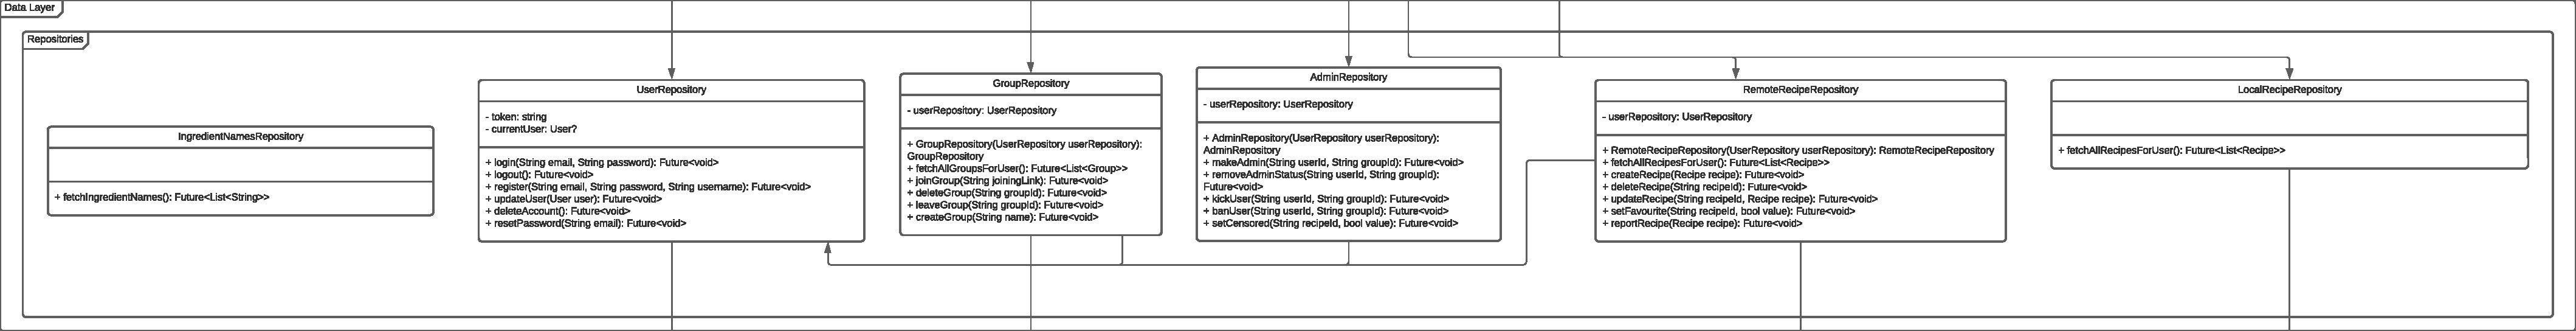
\includegraphics[width=\textwidth]{images/dataLayer/dataLayer.pdf}
    \caption{Klassendiagramm der Repository-Klassen}
    \label{fig:dataLayer}
\end{figure}
\newpage
\subsection{\texttt{IngredientNamesRepository}}
\label{sec:ingredientNamesRepository}
Das Repository stellt die Schnittstelle zwischen der Geschäftslogik und der Datenquelle für Zutatennamen dar. Es bietet eine Methode zum Abfragen der Daten.
\subsubsection*{Methoden}
\paragraph{\texttt{fetchIngredientNames(): Future<List<String>>}}
Stellt eine Anfrage zum Erhalt aller Zutatennamen an den Server. Gibt ein Future-Objekt zurück, das aufgelöst wird, sobald die Namen erhalten wurden.
\newpage

\subsection{\texttt{UserRepository}}
\label{sec:userRepository}
Das \texttt{UserRepository} stellt die Schnittstelle zwischen der Geschäftslogik und der Datenquelle für Nutzer dar. Es bietet Methoden zur Abfrage, Aktualisierung und Speicherung von Nutzern und speichert das Token zur Authentifizierung des Nutzers bei dem Server.
\subsubsection*{Attribute}
\paragraph{\texttt{idToken: String?}}
Das \glslink{id-token}{ID-Token} zur Authentifizierung des Nutzers mit dem Server. Es handelt sich um ein privates Attribut, das nur über einen Getter gelesen werden kann. Das Token entspricht dem \glslink{JWT}{JWT-Token}, das der Server nach der Authentifizierung des Nutzers zurückgibt. Darin sind unteranderem die Nutzer-ID und die Gültigkeitsdauer des Tokens kodiert enthalten. Das Token wird bei jeder Anfrage an den Server mitgeschickt, um den Nutzer zu authentifizieren.

\paragraph{\texttt{refreshToken: String?}}
Der \glslink{refresh-token}{Refresh-Token} zur Authentifizierung des Nutzers mit dem Server. Es handelt sich um ein privates Attribut, das nur über einen Getter gelesen werden kann. Das Token wird verwendet, um ein neues \glslink{id-token}{ID-Token} zu erhalten, wenn das alte abgelaufen ist. Das Token entspricht dem \glslink{JWT}{JWT-Token}, das der Server nach der Authentifizierung des Nutzers zurückgibt. Darin sind unteranderem die Nutzer-ID und die Gültigkeitsdauer des Tokens kodiert enthalten. Das Token wird bei jeder Anfrage an den Server mitgeschickt, um den Nutzer zu authentifizieren.

\subsubsection*{Methoden}
\paragraph{\texttt{getToken(): String}}
Gibt das Token zur Authentifizierung des Nutzers bei dem Server zurück.
\paragraph{\texttt{fetchCurrentUser(): Future<User?>}}
Fragt das User-Objekt eines Nutzers vom Server an. Gibt ein Future-Objekt zurück, das aufgelöst wird, wenn der Nutzer erhalten wurde. Ist der Nutzer nicht angemeldet, wird null zurückgegeben.
\paragraph{\texttt{login(String email, String password): Future<void>}}
Es wird eine Anfrage zum Nutzer Anmelden an den Server gestellt. Nimmt als Parameter die E-Mail-Adresse und das Passwort des Nutzers entgegen. Die Methode ist asynchron und gibt ein \texttt{Future}-Objekt zurück. Das \texttt{Future}-Objekt wird aufgelöst, wenn die Anmeldung erfolgreich war. Wenn die Anmeldung fehlschlägt, wird eine Exception geworfen. Die Methode speichert das Token in dem privaten Attribut \texttt{token} und das \texttt{User}-Objekt, das den aktuell angemeldeten Nutzer repräsentiert, in dem privaten Attribut \texttt{currentUser}.
\paragraph{\texttt{logout(): Future<void>}}
Es wird eine Anfrage an den Server zum Abmelden des Nutzers gestellt. Die Methode ist asynchron und gibt ein \texttt{Future}-Objekt zurück. Das \texttt{Future}-Objekt wird aufgelöst, wenn die Abmeldung erfolgreich war. Wenn die Abmeldung fehlschlägt, wird eine Exception geworfen. Die Methode löscht das Token aus dem privaten Attribut \texttt{token} und das \texttt{User}-Objekt aus dem privaten Attribut \texttt{currentUser}.
\paragraph{\texttt{register(String email, String password, String username): Future<void>}}
Stellt eine Anfrage an den Server, einen neuen Nutzer zu registrieren. Nimmt als Parameter die E-Mail-Adresse, das Passwort und den Nutzernamen des Nutzers entgegen. Die Methode ist asynchron und gibt ein \texttt{Future}-Objekt zurück. Das \texttt{Future}-Objekt wird aufgelöst, wenn die Registrierung erfolgreich war. Wenn die Registrierung fehlschlägt, wird eine Exception geworfen. Die Methode speichert das Token in dem privaten Attribut \texttt{token} und das \texttt{User}-Objekt, das den aktuell angemeldeten Nutzer repräsentiert, in dem privaten Attribut \texttt{currentUser}.
\paragraph{\texttt{updateUser(User user): Future<void>}}
Es wird eine Anfrage an den Server gesendet, den angemeldeten Nutzer zu aktualisieren. Die Methode aktualisiert das \texttt{User}-Objekt, das den aktuell angemeldeten Nutzer repräsentiert, in dem privaten Attribut \texttt{currentUser}.
Die Methode ist asynchron und gibt ein \texttt{Future}-Objekt zurück. Das \texttt{Future}-Objekt wird aufgelöst, wenn die Anfrage erfolgreich war. Wenn die Anfrage fehlschlägt, wird eine Exception geworfen.
\paragraph{deleteAccount(): Future<void>}
Es wird eine Anfrage an den Server gesendet, um den Account des aktuell angemeldeten Nutzers zu löschen. Die Methode ist asynchron und gibt ein \texttt{Future}-Objekt zurück. Das \texttt{Future}-Objekt wird aufgelöst, wenn die Anfrage erfolgreich war. Wenn die Anfrage fehlschlägt, wird eine Exception geworfen. Die Methode führt im Anschluss die Methode \texttt{logout()} aus.
\paragraph{resetPassword(String email): Future<void>}
Es wird eine Anfrage an den Server zum Zurücksetzen des Passworts gesendet. Nimmt als Parameter die E-Mail-Adresse des Nutzers entgegen. Die Methode ist asynchron und gibt ein \texttt{Future}-Objekt zurück. Das \texttt{Future}-Objekt wird aufgelöst, wenn der Server eine E-Mail zum Zurücksetzen des Passworts versendet hat. Wenn das Versenden fehlschlägt, wird eine Exception geworfen.

\newpage
\subsection{\texttt{GroupRepository}}
\label{sec:groupRepository}
Das \texttt{GroupRepository} stellt die Schnittstelle zwischen der Geschäftslogik und der Datenquelle für Gruppen dar. Es bietet Methoden zur Abfrage, Aktualisierung und Speicherung von Gruppen.
\subsubsection*{Attribute}
\paragraph{\texttt{userRepository: UserRepository}}
\texttt{UserRepository}-Objekt, welches das \texttt{GroupRepository}-Objekt verwendet. Es handelt sich um ein privates Attribut. Es wird später verwendet, um das Token zur Authentifizierung des Nutzers bei dem Server für Anfragen zu erhalten.
\subsubsection*{Methoden}
\paragraph{\texttt{GroupRepository(UserRepository userRepository): GroupRepository}}
Konstruktor. Initialisiert das Attribut \texttt{userRepository} mit dem übergebenen \texttt{UserRepository}-Objekt.
\paragraph{\texttt{fetchAllGroupsForUser(): Future<List<Group>>}}
Fragt alle Gruppen des aktuellen Nutzers beim Server an und gibt diese als Liste zurück. Die Methode ist asynchron und gibt ein \texttt{Future}-Objekt zurück. Das \texttt{Future}-Objekt wird aufgelöst, wenn die Abfrage erfolgreich war. Wenn die Abfrage fehlschlägt, wird eine Exception geworfen.
\paragraph{\texttt{joinGroup(String groupCode): Future<void>}}
Es wird eine Anfrage an den Server zum Beitritt des aktuellen Nutzers zu einer Gruppe mit dem übergebenen Beitrittslink gestellt. Nimmt als Parameter den Beitrittslink der Gruppe entgegen. Die Methode ist asynchron und gibt ein \texttt{Future}-Objekt zurück. Das \texttt{Future}-Objekt wird aufgelöst, wenn der Nutzer erfolgreich der Gruppe beigetreten ist. Wenn der Nutzer der Gruppe nicht beitreten kann, wird eine Exception geworfen.
\paragraph{\texttt{leaveGroup(String groupId): Future<void>}}
Es wird eine Anfrage an den Server zum Austritt des aktuellen Nutzers aus einer Gruppe mit der übergebenen Gruppen-ID gestellt. Nimmt als Parameter die ID der Gruppe entgegen. Die Methode ist asynchron und gibt ein \texttt{Future}-Objekt zurück. Das \texttt{Future}-Objekt wird aufgelöst, wenn der Nutzer erfolgreich die Gruppe verlassen hat. Wenn der Nutzer die Gruppe nicht verlassen kann, wird eine Exception geworfen.
\paragraph{\texttt{createGroup(String name): Future<void>}}
Es wird eine Anfrage an den Server zum Erstellen einer neuen Gruppe mit dem übergebenen Namen gestellt. Nimmt als Parameter den Namen der Gruppe entgegen. Die Methode ist asynchron und gibt ein \texttt{Future}-Objekt zurück. Das \texttt{Future}-Objekt wird aufgelöst, wenn die Gruppe erfolgreich erstellt wurde. Wenn die Gruppe nicht erstellt werden kann, wird eine Exception geworfen.
\paragraph{\texttt{updateGroup(String groupId, Group group): Future<void>}}
Es wird eine Anfrage an den Server zum Aktualisieren einer Gruppe mit der übergebenen Gruppen-ID gestellt. Nimmt als Parameter die ID der Gruppe und das aktualisierte Gruppen-Objekt entgegen. Die Methode ist asynchron und gibt ein \texttt{Future}-Objekt zurück. Das \texttt{Future}-Objekt wird aufgelöst, wenn die Gruppe erfolgreich aktualisiert wurde. Wenn die Gruppe nicht aktualisiert werden kann, wird eine Exception geworfen.
\paragraph{\texttt{deleteGroup(String groupId): Future<void>}}
Es wird eine Anfrage an den Server zum Löschen einer Gruppe mit der übergebenen Gruppen-ID gestellt. Nimmt als Parameter die ID der Gruppe entgegen. Die Methode ist asynchron und gibt ein \texttt{Future}-Objekt zurück. Das \texttt{Future}-Objekt wird aufgelöst, wenn die Gruppe erfolgreich gelöscht wurde. Wenn die Gruppe nicht gelöscht werden kann, wird eine Exception geworfen.
\newpage
\subsection{\texttt{AdminRepository}}
\label{sec:adminRepository}
Das \texttt{AdminRepository} stellt die Schnittstelle zwischen der Geschäftslogik und den Server-Schnittstellen für verschiedene Administratoraktionen dar.
\subsubsection*{Attribute}
\paragraph{\texttt{userRepository: UserRepository}}
\texttt{UserRepository}-Objekt, welches das \texttt{AdminRepository}-Objekt verwendet. Es handelt sich um ein privates Attribut. Es wird später verwendet, um das \glslink{id-token}{ID-Token} zur Authentifizierung des Nutzers bei dem Server für Anfragen zu erhalten.
\subsubsection*{Methoden}
\paragraph{\texttt{AdminRepository(UserRepository userRepository): AdminRepository}}
Konstruktor. Initialisiert das Attribut \texttt{userRepository} mit dem übergebenen \texttt{UserRepository}-Objekt.
\paragraph{\texttt{makeAdmin(String userId, String groupId): Future<void>}}
Es wird eine Anfrage an den Server gestellt, um den Nutzer mit der übergebenen ID zum Administrator der Gruppe mit der übergebenen ID zu machen. Nimmt als Parameter die ID des Nutzers und die ID der Gruppe entgegen. Die Methode ist asynchron und gibt ein \texttt{Future}-Objekt zurück. Das \texttt{Future}-Objekt wird aufgelöst, wenn der Nutzer erfolgreich zum Administrator der Gruppe gemacht wurde. Wenn der Nutzer nicht zum Administrator der Gruppe gemacht werden kann, wird eine Exception geworfen.
\paragraph{\texttt{removeAdminStatus(String userId, String groupId): Future<void>}}
Es wird eine Anfrage an den Server gestellt, um den Nutzer mit der übergebenen ID den Administratorstatus der Gruppe mit der übergebenen ID zu entziehen. Nimmt als Parameter die ID des Nutzers und die ID der Gruppe entgegen. Die Methode ist asynchron und gibt ein \texttt{Future}-Objekt zurück. Das \texttt{Future}-Objekt wird aufgelöst, wenn der Nutzer erfolgreich den Administratorstatus der Gruppe entzogen bekommen hat. Wenn der Nutzer nicht den Administratorstatus der Gruppe entzogen bekommen kann, wird eine Exception geworfen.
\paragraph{\texttt{kickUser(String userId, String groupId): Future<void>}}
Es wird eine Anfrage an den Server gestellt, um den Nutzer mit der übergebenen ID aus der Gruppe mit der übergebenen ID zu entfernen. Nimmt als Parameter die ID des Nutzers und die ID der Gruppe entgegen. Die Methode ist asynchron und gibt ein \texttt{Future}-Objekt zurück. Das \texttt{Future}-Objekt wird aufgelöst, wenn der Nutzer erfolgreich aus der Gruppe entfernt wurde. Wenn der Nutzer nicht aus der Gruppe entfernt werden kann, wird eine Exception geworfen.
\paragraph{\texttt{banUser(String userId, String groupId): Future<void>}}
Es wird eine Anfrage an den Server gestellt, um den Nutzer mit der übergebenen ID aus der Gruppe mit der übergebenen ID zu bannen. Nimmt als Parameter die ID des Nutzers und die ID der Gruppe entgegen. Die Methode ist asynchron und gibt ein \texttt{Future}-Objekt zurück. Das \texttt{Future}-Objekt wird aufgelöst, wenn der Nutzer erfolgreich aus der Gruppe gebannt wurde. Wenn der Nutzer nicht aus der Gruppe gebannt werden kann, wird eine Exception geworfen.
\paragraph{\texttt{setCensored(String recipeId, String groupId, bool value): Future<void>}}
Blendet das Rezept, das die gegebene ID besitzt, für die gegebene Gruppe aus. Nimmt als Parameter die ID des Rezepts und einen boolschen Wert, der angibt, ob das Rezept ausgeblendet oder entfernt werden soll, entgegen. Die Methode ist asynchron und gibt ein \texttt{Future}-Objekt zurück. Das \texttt{Future}-Objekt wird aufgelöst, wenn das Rezept erfolgreich ausgeblendet oder entfernt wurde. Wenn das Rezept nicht ausgeblendet oder entfernt werden kann, wird eine Exception geworfen.
\newpage
\subsection{\texttt{RemoteRecipeRepository}}\label{sec:remoteRecipeRepository}
Das \texttt{RemoteRecipeRepository} stellt die Schnittstelle zwischen der Geschäftslogik und den Server-Schnittstellen für Rezepte dar.
\subsubsection*{Attribute}
\paragraph{\texttt{userRepository: UserRepository}}
Das \texttt{UserRepository}-Objekt, welches von dem \texttt{Remote\-Recipe\-Repository}-Objekt verwendet wird. Es handelt sich um ein privates Attribut. Es wird später verwendet, um das Token zur Authentifizierung des Nutzers bei dem Server für Anfragen zu erhalten.
\subsubsection*{Methoden}
\paragraph{\texttt{RemoteRecipeRepository(UserRepository userRepository):RemoteRecipeRepository\\}}
Der Konstruktor der Klasse. Initialisiert das Attribut \texttt{userRepository} mit dem übergebenen \texttt{UserRepository}-Objekt.
\paragraph{\texttt{fetchAllRecipesForUser(): Future<List<Recipe>>}}
Fragt alle Rezepte aus Gruppen des aktuellen Nutzers vom Server ab. Nimmt keine Parameter entgegen. Die Methode ist asynchron und gibt ein \texttt{Future}-Objekt zurück. Das \texttt{Future}-Objekt wird aufgelöst, wenn die Rezepte erfolgreich vom Server abgefragt wurden. Wenn die Rezepte nicht vom Server abgefragt werden können, wird eine Exception geworfen. Speichert zudem alle Rezepte als JSON-Objekt via \Gls{SharedPreferences} in den lokalen Speicher.
\paragraph{\texttt{createRecipe(Recipe recipe): Future<void>}}
Erstellt ein neues Rezept auf dem Server. Nimmt als Parameter das Rezept, das erstellt werden soll, entgegen. Die Methode ist asynchron und gibt ein \texttt{Future}-Objekt zurück. Das \texttt{Future}-Objekt wird aufgelöst, wenn das Rezept erfolgreich erstellt wurde. Wenn das Rezept nicht erstellt werden kann, wird eine Exception geworfen.
\paragraph{\texttt{deleteRecipe(String recipeId): Future<void>}}
Löscht das Rezept mit der übergebenen ID vom Server. Nimmt als Parameter die ID des Rezepts entgegen. Die Methode ist asynchron und gibt ein \texttt{Future}-Objekt zurück. Das \texttt{Future}-Objekt wird aufgelöst, wenn das Rezept erfolgreich gelöscht wurde. Wenn das Rezept nicht gelöscht werden kann, wird eine Exception geworfen.
\paragraph{\texttt{updateRecipe(String recipeId, Recipe recipe): Future<void>}}
Ändert das Rezept mit der übergebenen ID auf dem Server. Nimmt als Parameter die ID des Rezepts und das aktualisierte Rezept entgegen. Die Methode ist asynchron und gibt ein \texttt{Future}-Objekt zurück. Das \texttt{Future}-Objekt wird aufgelöst, wenn das Rezept erfolgreich aktualisiert wurde. Wenn das Rezept nicht aktualisiert werden kann, wird eine Exception geworfen.
\paragraph{\texttt{setFavourite(String recipeId, bool value): Future<void>}}
Setzt das Rezept mit der übergebenen ID als Favorit des aktuellen Nutzers. Nimmt als Parameter die ID des Rezepts und einen boolschen Wert, der angibt, ob das Rezept als Favorit gesetzt oder entfernt werden soll, entgegen. Die Methode ist asynchron und gibt ein \texttt{Future}-Objekt zurück. Das \texttt{Future}-Objekt wird aufgelöst, wenn das Rezept erfolgreich als Favorit gesetzt oder entfernt wurde. Wenn das Rezept nicht als Favorit gesetzt oder entfernt werden kann, wird eine Exception geworfen.
\paragraph{\texttt{reportRecipe(String recipeId): Future<void>}}
Leitet die Anfrage zum Melden eines Rezepts an den Server. Nimmt als Parameter die ID des Rezepts entgegen. Die Methode ist asynchron und gibt ein \texttt{Future}-Objekt zurück. Das \texttt{Future}-Objekt wird aufgelöst, wenn das Rezept erfolgreich gemeldet wurde. Wenn das Rezept nicht gemeldet werden kann, wird eine Exception geworfen.
\newpage
\subsection{\texttt{LocalRecipeRepository}}
\label{sec:localRecipeRepository}
Das \texttt{LocalRecipeRepository} stellt die Schnittstelle zwischen der Geschäftslogik und dem lokalen Speicher für Rezepte dar.
\subsubsection*{Methoden}
\paragraph{\texttt{fetchAllRecipesForUser(): Future<List<Recipe>>}}
Fragt alle Rezepte aus Gruppen des aktuellen Nutzers aus dem lokalen Speicher via \Gls{SharedPreferences} ab. Nimmt keine Parameter entgegen. Die Methode ist asynchron und gibt ein \texttt{Future}-Objekt zurück. Das \texttt{Future}-Objekt wird aufgelöst, wenn die Rezepte erfolgreich aus dem lokalen Speicher abgefragt wurden. Wenn die Rezepte nicht aus dem lokalen Speicher abgefragt werden können, wird eine Exception geworfen.
\newpage
\section{Riverpod und Provider}
\label{sec:riverpod}
\subsection{Riverpod}
Der Sinn von Riverpod liegt darin, die Verwaltung von Zuständen und Abhängigkeiten in Flutter-Apps zu vereinfachen. Riverpod ist eine leistungsstarke und benutzerfreundliche State-Management-Bibliothek, die auf dem Konzept von "\nameref{sec:provider}" basiert. Mit Riverpod können Entwickler effizient und flexibel Zustände verwalten, Dienste bereitstellen und Abhängigkeiten zwischen verschiedenen Teilen der App verknüpfen. Dies erleichtert die Skalierbarkeit, Wiederverwendbarkeit und Testbarkeit von Flutter-Apps, da der Code klar strukturiert ist und das Trennen von Zuständen und UI-Logik erleichtert wird. Riverpod bietet eine intuitive Syntax, unterstützt einen deklarativen Ansatz zur Definition von Providern und ermöglicht das einfache Aktualisieren von Zuständen durch Nutzung des \glslink{Observer}{Observer-Konzepts}. Insgesamt erleichtert Riverpod die Entwicklung von Flutter-Apps und trägt dazu bei, den Code sauberer, wartbarer und effizienter zu gestalten.
\subsection{Provider}\label{sec:provider}
Provider sind spezielle Objekte, die dazu dienen, Werte oder Abhängigkeiten in Flutter-Apps bereitzustellen. Sie fungieren als eine Art Container, der den Zugriff auf diese Werte oder Dienste innerhalb der App ermöglicht.

Es gibt viele verschiedene Arten von Providern, die für verschiedene Zwecke verwendet werden können. In der Applikation werden die folgenden Provider-Arten verwendet:

\paragraph{\texttt{Provider}}
Der \texttt{Provider} stellt einen Wert bereit, der in der gesamten App verwendet werden kann. Dies kann beispielsweise ein Zustandswert, ein Konfigurationswert oder ein Dienstobjekt sein.

\paragraph{\texttt{AsyncNotifierProvider}}
Der \texttt{AsyncNotifierProvider} ist eine spezielle Art von Provider, der einen Zustandswert bereitstellt, der asynchron aktualisiert werden kann. Dies ist nützlich, wenn der Wert von einer asynchronen Operation abhängt, z.B. einer Datenabfrage von einer API. Durch ihn kann eine automatische Aktualisierung der Daten veranlasst werden, wenn beispielsweise eine API-Anfrage abgeschlossen wurde.

Provider werden in der Hierarchie der Flutter-Widgets platziert und können über den Widget-Tree hinweg zugänglich gemacht werden. Dadurch können sie in verschiedenen Teilen der App genutzt werden, indem sie mit dem entsprechenden Provider verbunden werden.

Die Verwendung von Providern in Riverpod ermöglicht eine saubere Trennung von Zuständen und Logik, fördert die Wiederverwendbarkeit und erleichtert das Testen von Flutter-Apps.

Es wird für jede Repository-Klasse ein eigener Provider vom Typ \texttt{Provider} erstellt. Zudem erhält jeder Service einen eigenen \texttt{AsyncNotifierProvider}. Mehr zu der Funktionsweise des \texttt{AsyncNotifierProvider} mit den Services ist in Kapitel \ref{sec:asyncNotifier} zu finden.

\newpage
\section{Application Layer}
Der Application Layer ist eine weitere wichtige Komponente einer Smartphone-App. Seine Hauptaufgabe besteht darin, die Geschäftslogik der Anwendung zu implementieren und die Kernfunktionalität zu verwalten. Der Application Layer enthält verschiedene Klassen und Methoden, die die Regeln und Abläufe der Anwendung definieren. Er ist unabhängig von der Benutzeroberfläche und den spezifischen Details der Datenpersistenz. Stattdessen konzentriert sich der Application Layer darauf, die Kernfunktionalität der App zu modellieren und sicherzustellen, dass diese korrekt und effizient ausgeführt wird. Dadurch wird die Wiederverwendbarkeit, Testbarkeit und Flexibilität der Anwendung verbessert. Der Application Layer fungiert als Vermittler zwischen dem \nameref{sec:presentationLayer} und dem \nameref{sec:dataLayer} und ermöglicht eine saubere Trennung der Verantwortlichkeiten in der App-Architektur.
Er enthält in erster Linie viele verschiedene Services, die die verschiedenen Entitäten verwalten.
\begin{figure}[htp]
    \centering
    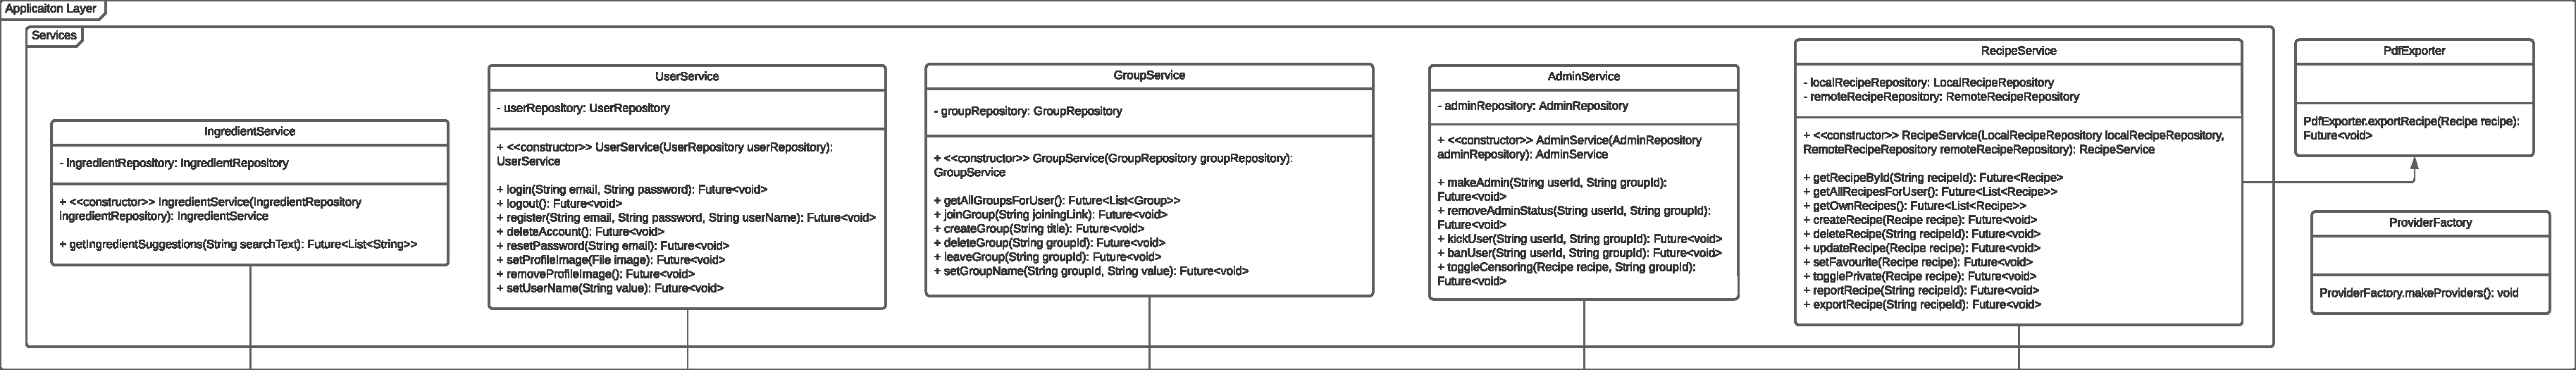
\includegraphics[width = \textwidth]{images/applicationLayer/applicationLayer.pdf}
    \caption{Klassendiagramm des Application Layer}
    \label{fig:application-layer}
\end{figure}

Nun werden die einzelnen Klassen des Application Layers beschrieben.
\newpage
\subsection{\texttt{AsyncNotifier<T>}}
\label{sec:asyncNotifier}
Die Klasse ist Teil von Riverpod. Sie ermöglicht es Zustände asynchron zu aktualisieren. Dies ist nützlich, wenn der Wert von einer asynchronen Operation abhängt, z.B. einer Datenabfrage von einer API. Durch ihn kann eine automatische Aktualisierung der Daten veranlasst werden, wenn beispielsweise eine API-Anfrage abgeschlossen wurde.
\subsubsection*{Attribute}
\paragraph{\texttt{state: AsyncValue<T>}}
Der Zustand, der durch den \texttt{AsyncNotifier} verwaltet wird. Er ist privat und kann nur über die Methoden der Klasse geändert werden. Wird das Attribut verändert, werden alle UI-Elemente, die mit dem \texttt{AsyncNotifier} verbunden sind, infomiert und gegebenenfalls aktualisiert.
\subsubsection*{Methoden}
\paragraph{\texttt{build(): FutureOr<T>}}
Abstrakte Methode, die in den Unterklassen implementiert werden muss. Der Rückgabewert legt den Initialwert des Zustands fest.
\newpage
\subsection{\texttt{UserService}}
\label{sec:userService}
Der Service dient dazu, die Nutzer zu verwalten. Er erbt von der Klasse \texttt{AsyncNotifier<User?>}. Das Attribut \texttt{state} enthält, immer wenn Daten verfügbar sind, den aktuellen Nutzer oder \texttt{null}, wenn kein Nutzer angemeldet ist.

\subsubsection*{Attribute}
\paragraph{\texttt{userRepository: UserRepository}}
Das \texttt{UserRepository}, das zum Zugriff auf die Nutzer verwendet wird. Es wird im Konstruktor initialisiert und ist privat.
\subsubsection*{Methoden}
\paragraph{\texttt{UserService(UserRepository userRepository): UserService}}
Konstruktor für die Klasse. Initialisiert das \texttt{UserRepository}, das zum Zugriff auf die Nutzer verwendet wird. Nimmt als Parameter das \texttt{UserRepository} entgegen.
\paragraph{\texttt{build(): FutureOr<User?>}}
Implementiert die abstrakte Methode \texttt{build()} der Klasse \\ \texttt{Async\-Notifier}. Gibt den Initialwert des Zustands zurück. In diesem Fall ist der Initialwert der angemeldete Nutzer, falls er angemeldet ist.
\paragraph{\texttt{login(String email, String password): Future<void>}}
Leitet die Loginanfrage an das zuständige Repository weiter. Nimmt als Parameter die E-Mail-Adresse und das Passwort des Nutzers entgegen. Die Methode ist asynchron und gibt ein \texttt{Future}-Objekt zurück. Das \texttt{Future}-Objekt wird aufgelöst, wenn der Nutzer erfolgreich eingeloggt wurde. Wenn der Nutzer nicht eingeloggt werden kann, wird eine Exception geworfen. Der Nutzer wird in dem Attribut \texttt{state} gespeichert.
\paragraph{\texttt{logout(): Future<void>}}
Leitet die Logout-Anfrage an das zuständige Repository weiter. Nimmt keine Parameter entgegen. Die Methode ist asynchron und gibt ein \texttt{Future}-Objekt zurück. Das \texttt{Future}-Objekt wird aufgelöst, wenn der Nutzer erfolgreich ausgeloggt wurde. Wenn der Nutzer nicht ausgeloggt werden kann, wird eine Exception geworfen. Der Nutzer wird aus dem Attribut \texttt{state} entfernt.
\paragraph{\texttt{register(String email, String password): Future<void>}}
Leitet die Registrierungs-An\-frage an das zuständige Repository weiter. Nimmt als Parameter die E-Mail-Adresse und das Passwort des Nutzers entgegen. Die Methode ist asynchron und gibt ein \texttt{Future}-Objekt zurück. Das \texttt{Future}-Objekt wird aufgelöst, wenn der Nutzer erfolgreich registriert wurde. Wenn der Nutzer nicht registriert werden kann, wird eine Exception geworfen. Der Nutzer wird in dem Attribut \texttt{state} gespeichert.
\paragraph{\texttt{deleteAccount(): Future<void>}}
Leitet die Anfrage zum Löschen des Nutzerkontos an das zuständige Repository weiter. Nimmt keine Parameter entgegen. Die Methode ist asynchron und gibt ein \texttt{Future}-Objekt zurück. Das \texttt{Future}-Objekt wird aufgelöst, wenn das Nutzerkonto erfolgreich gelöscht wurde. Wenn das Nutzerkonto nicht gelöscht werden kann, wird eine Exception geworfen. Der Nutzer wird aus dem Attribut \texttt{state} entfernt.
\paragraph{\texttt{resetPassword(String email): Future<void>}}
Leitet die Anfrage zum Zurücksetzen des Passworts an das zuständige Repository weiter. Nimmt als Parameter die E-Mail-Adresse des Nutzers entgegen. Die Methode ist asynchron und gibt ein \texttt{Future}-Objekt zurück. Das \texttt{Future}-Objekt wird aufgelöst, wenn das Passwort erfolgreich zurückgesetzt wurde. Wenn das Passwort nicht zurückgesetzt werden kann, wird eine Exception geworfen.
\paragraph{\texttt{setProfileImage(File image): Future<void>}}
Leitet eine Anfrage zum Aktualisieren des Nutzers an das zuständige Repository weiter, indem ein \texttt{User}-Objekt mit verändertem Profilbild erzeugt wird. Nimmt als Parameter ein \texttt{File}-Objekt entgegen, das das neue Profilbild des Nutzers darstellt. Die Methode ist asynchron und gibt ein \texttt{Future}-Objekt zurück. Das \texttt{Future}-Objekt wird aufgelöst, wenn das Profilbild erfolgreich aktualisiert wurde. Wenn das Profilbild nicht aktualisiert werden kann, wird eine Exception geworfen. Der aktualisierte Nutzer wird in dem Attribut \texttt{state} gespeichert.
\paragraph{\texttt{removeProfileImage(): Future<void>}}
Leitet eine Anfrage zum Aktualisieren des Nutzers an das zuständige Repository weiter, indem ein \texttt{User}-Objekt ohne Profilbild erzeugt wird. Nimmt keine Parameter entgegen. Die Methode ist asynchron und gibt ein \texttt{Future}-Objekt zurück. Das \texttt{Future}-Objekt wird aufgelöst, wenn das Profilbild erfolgreich aktualisiert wurde. Wenn das Profilbild nicht aktualisiert werden kann, wird eine Exception geworfen. Der aktualisierte Nutzer wird in dem Attribut \texttt{state} gespeichert.
\paragraph{\texttt{setUserName(String value): Future<void>}}
Stellt eine Anfrage zum Aktualisieren des Nutzers an das zuständige Repository, indem ein \texttt{User}-Objekt mit verändertem Nutzernamen erzeugt wird. Nimmt als Parameter eine Zeichenkette entgegen, die den neuen Nutzernamen darstellt. Die Methode ist asynchron und gibt ein \texttt{Future}-Objekt zurück. Das \texttt{Future}-Objekt wird aufgelöst, wenn der Nutzername erfolgreich aktualisiert wurde. Wenn der Nutzername nicht aktualisiert werden kann, wird eine Exception geworfen. Der aktualisierte Nutzer wird in dem Attribut \texttt{state} gespeichert.

\newpage
\subsection{\texttt{GroupService}}
\label{sec:groupService}
Der Service dient dazu, die Gruppen zu verwalten. Er erbt von der Klasse \texttt{AsyncNotifier<List <Group>>}. Das Attribut \texttt{state} enthält, immer wenn Daten verfügbar sind, alle Gruppen des aktuellen Nutzers.
\subsubsection*{Attribute}
\paragraph{\texttt{groupRepository: GroupRepository}}
Das \texttt{GroupRepository}, das zum Zugriff auf die Gruppen verwendet wird. Es wird im Konstruktor initialisiert und ist privat.
\paragraph{\texttt{adminRepository: AdminRepository}}
Das \texttt{AdminRepository}, das zum Zugriff auf die Administratoraktionen verwendet wird. Es wird im Konstruktor initialisiert und ist privat.
\subsubsection*{Methoden}
\paragraph{\texttt{GroupService(GroupRepository groupRepository): GroupService}}
Konstruktor. Initialisiert das \texttt{GroupRepository}, das zum Zugriff auf die Gruppen verwendet wird, und das \texttt{AdminRe\-pository}, das zum Zugriff auf die Administratoraktionen dient. Nimmt als Parameter die beiden Repositorys entgegen.
\paragraph{\texttt{build(): FutureOr<List<Group>>}}
Implementiert die abstrakte Methode \texttt{build()} der Klasse \texttt{AsyncNotifier}. Gibt den Initialwert des Zustands zurück. In diesem Fall ist der Initialwert \texttt{groupRepository.fetchAllGroupsForUser()}.
\paragraph{\texttt{joinGroup(String groupCode): Future<void>}}
Leitet die Anfrage zum Beitreten einer Gruppe an das zuständige Repository weiter. Fragt im Anschluss erneut die Gruppen des Nutzers ab und aktualisiert den \texttt{state}. Nimmt als Parameter das Gruppenkürzel der Gruppe entgegen. Die Methode ist asynchron und gibt ein \texttt{Future}-Objekt zurück. Das \texttt{Future}-Objekt wird aufgelöst, wenn der Nutzer erfolgreich der Gruppe beigetreten ist. Wenn der Nutzer nicht der Gruppe beitreten kann, wird eine Exception geworfen.
\paragraph{\texttt{createGroup(String groupName): Future<void>}}
Leitet die Anfrage zum Erstellen einer Gruppe an das zuständige Repository weiter. Fragt im Anschluss erneut die Gruppen des Nutzers ab und aktualisiert den \texttt{state}. Nimmt als Parameter den Namen der Gruppe entgegen. Die Methode ist asynchron und gibt ein \texttt{Future}-Objekt zurück. Das \texttt{Future}-Objekt wird aufgelöst, wenn die Gruppe erfolgreich erstellt wurde. Wenn die Gruppe nicht erstellt werden kann, wird eine Exception geworfen.
\paragraph{\texttt{deleteGroup(String groupId): Future<void>}}
Leitet die Anfrage zum Löschen einer Gruppe an das zuständige Repository weiter. Fragt im Anschluss erneut die Gruppen des Nutzers ab und aktualisiert den \texttt{state}. Nimmt als Parameter die ID der Gruppe entgegen. Die Methode ist asynchron und gibt ein \texttt{Future}-Objekt zurück. Das \texttt{Future}-Objekt wird aufgelöst, wenn die Gruppe erfolgreich gelöscht wurde. Wenn die Gruppe nicht gelöscht werden kann, wird eine Exception geworfen.
\paragraph{\texttt{leaveGroup(String groupId): Future<void>}}
Leitet die Anfrage zum Verlassen einer Gruppe an das zuständige Repository weiter. Fragt im Anschluss erneut die Gruppen des Nutzers ab und aktualisiert den \texttt{state}. Nimmt als Parameter die ID der Gruppe entgegen. Die Methode ist asynchron und gibt ein \texttt{Future}-Objekt zurück. Das \texttt{Future}-Objekt wird aufgelöst, wenn der Nutzer erfolgreich die Gruppe verlassen hat. Wenn der Nutzer die Gruppe nicht verlassen kann, wird eine Exception geworfen.
\paragraph{\texttt{setGroupName(String groupId, String groupName): Future<void>}}
Stellt eine Anfrage, um eine Gruppe zu aktualisieren, an das zuständige Repository, indem ein neues \texttt{Group}-Objekt mit aktualisiertem Namen erzeugt wird. Fragt im Anschluss erneut die Gruppen des Nutzers ab und aktualisiert den \texttt{state}. Nimmt als Parameter die ID der Gruppe und den neuen Namen der Gruppe entgegen. Die Methode ist asynchron und gibt ein \texttt{Future}-Objekt zurück. Das \texttt{Future}-Objekt wird aufgelöst, wenn die Gruppe erfolgreich aktualisiert wurde. Wenn die Gruppe nicht aktualisiert werden kann, wird eine Exception geworfen.
\paragraph{\texttt{makeAdmin(String userId, String groupId): Future<void>}}
Leitet die Anfrage zum Ernennen eines Nutzers zum Administrator einer Gruppe an das zuständige Repository weiter. Fragt im Anschluss erneut die Gruppen des Nutzers ab und aktualisiert den \texttt{state}. Nimmt als Parameter die ID des Nutzers und die ID der Gruppe entgegen. Die Methode ist asynchron und gibt ein \texttt{Future}-Objekt zurück. Das \texttt{Future}-Objekt wird aufgelöst, wenn der Nutzer erfolgreich zum Administrator ernannt wurde. Wenn der Nutzer nicht zum Administrator ernannt werden kann, wird eine Exception geworfen.
\paragraph{\texttt{removeAdminStatus(String userId, String groupId): Future<void>}}
Leitet die Anfrage zum Entfernen des Administratorstatus eines Nutzers einer Gruppe an das zuständige Repository weiter. Fragt im Anschluss erneut die Gruppen des Nutzers ab und aktualisiert den \texttt{state}. Nimmt als Parameter die ID des Nutzers und die ID der Gruppe entgegen. Die Methode ist asynchron und gibt ein \texttt{Future}-Objekt zurück. Das \texttt{Future}-Objekt wird aufgelöst, wenn der Administratorstatus des Nutzers erfolgreich entfernt wurde. Wenn der Administratorstatus des Nutzers nicht entfernt werden kann, wird eine Exception geworfen.
\paragraph{\texttt{kickUser(String userId, String groupId): Future<void>}}
Leitet die Anfrage zum Entfernen eines Nutzers aus einer Gruppe an das zuständige Repository weiter. Fragt im Anschluss erneut die Gruppen des Nutzers ab und aktualisiert den \texttt{state}. Nimmt als Parameter die ID des Nutzers und die ID der Gruppe entgegen. Die Methode ist asynchron und gibt ein \texttt{Future}-Objekt zurück. Das \texttt{Future}-Objekt wird aufgelöst, wenn der Nutzer erfolgreich aus der Gruppe entfernt wurde. Wenn der Nutzer nicht aus der Gruppe entfernt werden kann, wird eine Exception geworfen.
\paragraph{\texttt{banUser(String userId, String groupId): Future<void>}}
Leitet die Anfrage zum Bannen eines Nutzers aus einer Gruppe an das zuständige Repository weiter. Fragt im Anschluss erneut die Gruppen des Nutzers ab und aktualisiert den \texttt{state}. Nimmt als Parameter die ID des Nutzers und die ID der Gruppe entgegen. Die Methode ist asynchron und gibt ein \texttt{Future}-Objekt zurück. Das \texttt{Future}-Objekt wird aufgelöst, wenn der Nutzer erfolgreich aus der Gruppe gebannt wurde. Wenn der Nutzer nicht aus der Gruppe gebannt werden kann, wird eine Exception geworfen.
\paragraph{\texttt{toggleCensoring(Recipe recipe, String groupId): Future<void>}}
Stellt eine Anfrage, um das \glslink{ausblenden}{Ausblenden} eines Rezeptes in einer Gruppe zu aktivieren/deaktivieren, an das zuständige Repository. Fragt im Anschluss erneut die Gruppen des Nutzers ab und aktualisiert den \texttt{state}. Nimmt als Parameter das Rezept und die ID der Gruppe entgegen. Die Methode ist asynchron und gibt ein \texttt{Future}-Objekt zurück. Das \texttt{Future}-Objekt wird aufgelöst, wenn das Aublenden des Rezepts erfolgreich de-/aktiviert wurde. Wenn das Ausblenden des Rezepts nicht geändert werden kann, wird eine Exception geworfen.

\newpage
\subsection{\texttt{RecipeService}}
\label{sec:recipeService}
Der Service dient dazu, die Rezepte zu verwalten. Er erbt von der Klasse \texttt{AsyncNotifier<void>}. Das Attribut \texttt{state} enthält, immer wenn Daten verfügbar sind, die Liste der Rezepte, die der angemeldete Nutzer sehen darf.
\subsubsection*{Attribute}
\paragraph{\texttt{localRecipeRepository: LocalRecipeRepository}}
Das Repository, das zum Zugriff auf die Rezepte im Systemspeicher verwendet wird. Es wird im Konstruktor initialisiert und ist privat. Besteht keine Verbindung zum Internet wird dieses Repository von den Methoden angesteuert.
\paragraph{\texttt{remoteRecipeRepository: RemoteRecipeRepository}}
Das Repository, das zum Zugriff auf die Rezepte in der Datenbank verwendet wird. Es wird im Konstruktor initialisiert und ist privat. Besteht eine Verbindung zum Internet wird dieses Repository von den Methoden angesteuert.
\subsubsection*{Methoden}
\paragraph{\texttt{RecipeService(LocalRecipeRepository localRecipeRepository, RemoteRecipeRepository remoteRecipeRepository): RecipeService\\}}
Konstruktor. Initialisiert die Repositories, die zum Zugriff auf die Rezepte verwendet werden. Nimmt als Parameter das \texttt{LocalRecipeReposi\-tory} und das \texttt{RemoteRecipeRepository} entgegen.
\paragraph{\texttt{build: FutureOr<List<Recipe>>}}
Implementiert die abstrakte Methode \texttt{build()} der Klasse \texttt{AsyncNotifier}.
Gibt den Initialwert des Zustands zurück. In diesem Fall ist der Initialwert je nach Verbindung \texttt{localRecipeRepository.fetchAllGroupsForUser()} oder \texttt{remoteRecipeRe\-pository.fetchAllGroupsForUser()}.
\paragraph{\texttt{createRecipe(Recipe recipe): Future<void>}}
Leitet die Anfrage zum Erstellen eines Rezepts an das zuständige Repository weiter. Fragt im Anschluss erneut die Rezepte für den Nutzer ab und aktualisiert den \texttt{state}. Nimmt als Parameter das Rezept entgegen. Die Methode ist asynchron und gibt ein \texttt{Future}-Objekt zurück. Das \texttt{Future}-Objekt wird aufgelöst, wenn das Rezept erfolgreich erstellt wurde. Wenn das Rezept nicht erstellt werden kann, wird eine Exception geworfen.
\paragraph{\texttt{deleteRecipe(String recipeId)}}
Leitet die Anfrage zum Löschen eines Rezepts an das zuständige Repository weiter. Fragt im Anschluss erneut die Rezepte für den Nutzer ab und aktualisiert den \texttt{state}. Nimmt als Parameter die ID des Rezepts entgegen. Die Methode ist asynchron und gibt ein \texttt{Future}-Objekt zurück. Das \texttt{Future}-Objekt wird aufgelöst, wenn das Rezept erfolgreich gelöscht wurde. Wenn das Rezept nicht gelöscht werden kann, wird eine Exception geworfen.
\paragraph{\texttt{updateRecipe(Recipe recipe): Future<void>}}
Leitet die Anfrage zum Aktualisieren eines Rezepts an das zuständige Repository weiter. Fragt im Anschluss erneut die Rezepte für den Nutzer ab und aktualisiert den \texttt{state}. Nimmt als Parameter das Rezept mit den bereits aktualisierten Werten entgegen. Die Methode ist asynchron und gibt ein \texttt{Future}-Objekt zurück. Das \texttt{Future}-Objekt wird aufgelöst, wenn das Rezept erfolgreich aktualisiert wurde. Wenn das Rezept nicht aktualisiert werden kann, wird eine Exception geworfen.
\paragraph{\texttt{toggleFavourite(Recipe recipe): Future<void>}}
Leitet die Anfrage zum Aktivieren/De\-aktivieren eines Rezepts als Favorit an das zuständige Repository weiter. Fragt im Anschluss erneut die Rezepte für den Nutzer ab und aktualisiert den \texttt{state}. Nimmt als Parameter das Rezept entgegen. Die Methode ist asynchron und gibt ein \texttt{Future}-Objekt zurück. Das \texttt{Future}-Objekt wird aufgelöst, wenn das Rezept erfolgreich als Favorit markiert wurde. Wenn das Rezept nicht als Favorit markiert werden kann, wird eine Exception geworfen.
\paragraph{\texttt{togglePrivate(Recipe recipe): Future<void>}}
Leitet die Anfrage zum Aktivieren/Deak\-ti\-vieren eines Rezepts als privat an das zuständige Repository weiter. Fragt im Anschluss erneut die Rezepte für den Nutzer ab und aktualisiert den \texttt{state}. Nimmt als Parameter das Rezept entgegen. Die Methode ist asynchron und gibt ein \texttt{Future}-Objekt zurück. Das \texttt{Future}-Objekt wird aufgelöst, wenn das Rezept erfolgreich als privat markiert wurde. Wenn das Rezept nicht als privat markiert werden kann, wird eine Exception geworfen.
\paragraph{\texttt{reportRecipe(String recipeId): Future<void>}}
Leitet die Anfrage zum Melden eines Rezepts an das zuständige Repository weiter. Nimmt als Parameter die ID des Rezepts entgegen. Die Methode ist asynchron und gibt ein \texttt{Future}-Objekt zurück. Das \texttt{Future}-Objekt wird aufgelöst, wenn das Rezept erfolgreich gemeldet wurde. Wenn das Rezept nicht gemeldet werden kann, wird eine Exception geworfen.
\paragraph{\texttt{exportRecipe(Recipe recipe): Future<void>}}
Erstellt eine PDF-Datei mit Hilfe der Klasse \texttt{PdfExporter}. Nimmt als Parameter das Rezept entgegen. Die Methode ist asynchron und gibt ein \texttt{Future}-Objekt zurück. Das \texttt{Future}-Objekt wird aufgelöst, wenn die PDF-Datei erfolgreich erstellt wurde. Wenn die PDF-Datei nicht erstellt werden kann, wird eine Exception geworfen.

\newpage
\subsection{\texttt{PdfExporter}}
\label{sec:pdfExporter}
Der \texttt{PdfExporter} dient dazu, ein Template und Methoden zur Verfügung zu stellen, um ein Rezept als PDF-Datei zu exportieren.
\subsubsection*{Methoden}
\paragraph{\texttt{PdfExporter.exportRecipe(Recipe recipe): Future<void>}}
Erstellt eine PDF-Datei, die das Rezept enthält und exportiert dieses anschließend. Nimmt als Parameter das Rezept entgegen. Die Methode ist asynchron und gibt ein \texttt{Future}-Objekt zurück. Das \texttt{Future}-Objekt wird aufgelöst, wenn die PDF-Datei erfolgreich erstellt und exportiert wurde. Wenn die PDF-Datei nicht erstellt und exportiert werden kann, wird eine Exception geworfen.
\newpage
\section{Presentation Layer}\label{sec:presentationLayer}
Der Presentation Layer in der Android-App-Entwicklung ist für die Darstellung der Benutzeroberfläche (UI) und die Kommunikation mit dem Benutzer verantwortlich. Er fungiert als Bindeglied zwischen dem Benutzer und den darunterliegenden Schichten wie der Datenquelle und der Geschäftslogik. Die Hauptaufgabe des Presentation Layers besteht darin, die Benutzerinteraktion zu ermöglichen, Benutzereingaben zu verarbeiten, Daten aus anderen Schichten abzurufen und anzuzeigen, und Feedback an den Benutzer zu liefern. Es umfasst die Aktivitäten, Zustände und Teilansichten, die zur Darstellung der UI verwendet werden. Der Zweck des Presentation Layers besteht darin, eine benutzerfreundliche und ansprechende Benutzeroberfläche bereitzustellen, die die Benutzererfahrung optimiert und eine effektive Kommunikation zwischen Benutzer und Anwendung ermöglicht. Durch eine klare Trennung des Presentation Layers von anderen Schichten kann die Wartbarkeit, Testbarkeit und Wiederverwendbarkeit der App verbessert werden.

In den folgenden Klassendiagrammen wurden zur Übersichtlichkeit Assoziationen zum Domain Layer weggelassen. Sie werden jedoch als Attribut aufgeführt und im zugehörigen Text beschrieben. Zudem wurden drei Schlüsselwörter benutzt, die nun erläutert werden sollen.

\paragraph{<<StatelessWidget>>}
Impliziert, das die Klasse mit diesem Schlüsselwort von der Flutterklasse \texttt{StatelessWidget} erbt. Dieses besitzt verschiedene Methoden, die die Darstellung des Widgets ermöglichen. Die wichtigste Methode ist \texttt{build}, die das Widget zurückgibt, welches dargestellt werden soll.
\paragraph{<<StatefulWidget>>}
Impliziert, das die Klasse mit diesem Schlüsselwort von der Flutterklasse \texttt{StatefulWidget} erbt. Diese Klasse besitzt zusätzlich eine \texttt{State}-Klasse, die die Zustände des Widgets verwaltet. Die Klasse \texttt{State} besitzt die Methode \texttt{build}, die das Widget zurückgibt, welches dargestellt werden soll. Da die vielen State-Klassen, das Klassendiagramm stark unübersichtlich machen würden, jedoch einfach zu implementieren und zu verstehen sind, wurden diese weggelassen.
\paragraph{<<FlutterWidget>>} Klassen mit diesem Schlüsselwort stammen aus dem Flutter-Framework. Sie werden nur verwendet, um Vererbungen zu verdeutlichen und daher wurden Attribute weggelassen. Bei Bedarf können sie in der Flutter-Dokumentation nachgeschlagen werden.
\begin{figure}[htp]
    \centering
    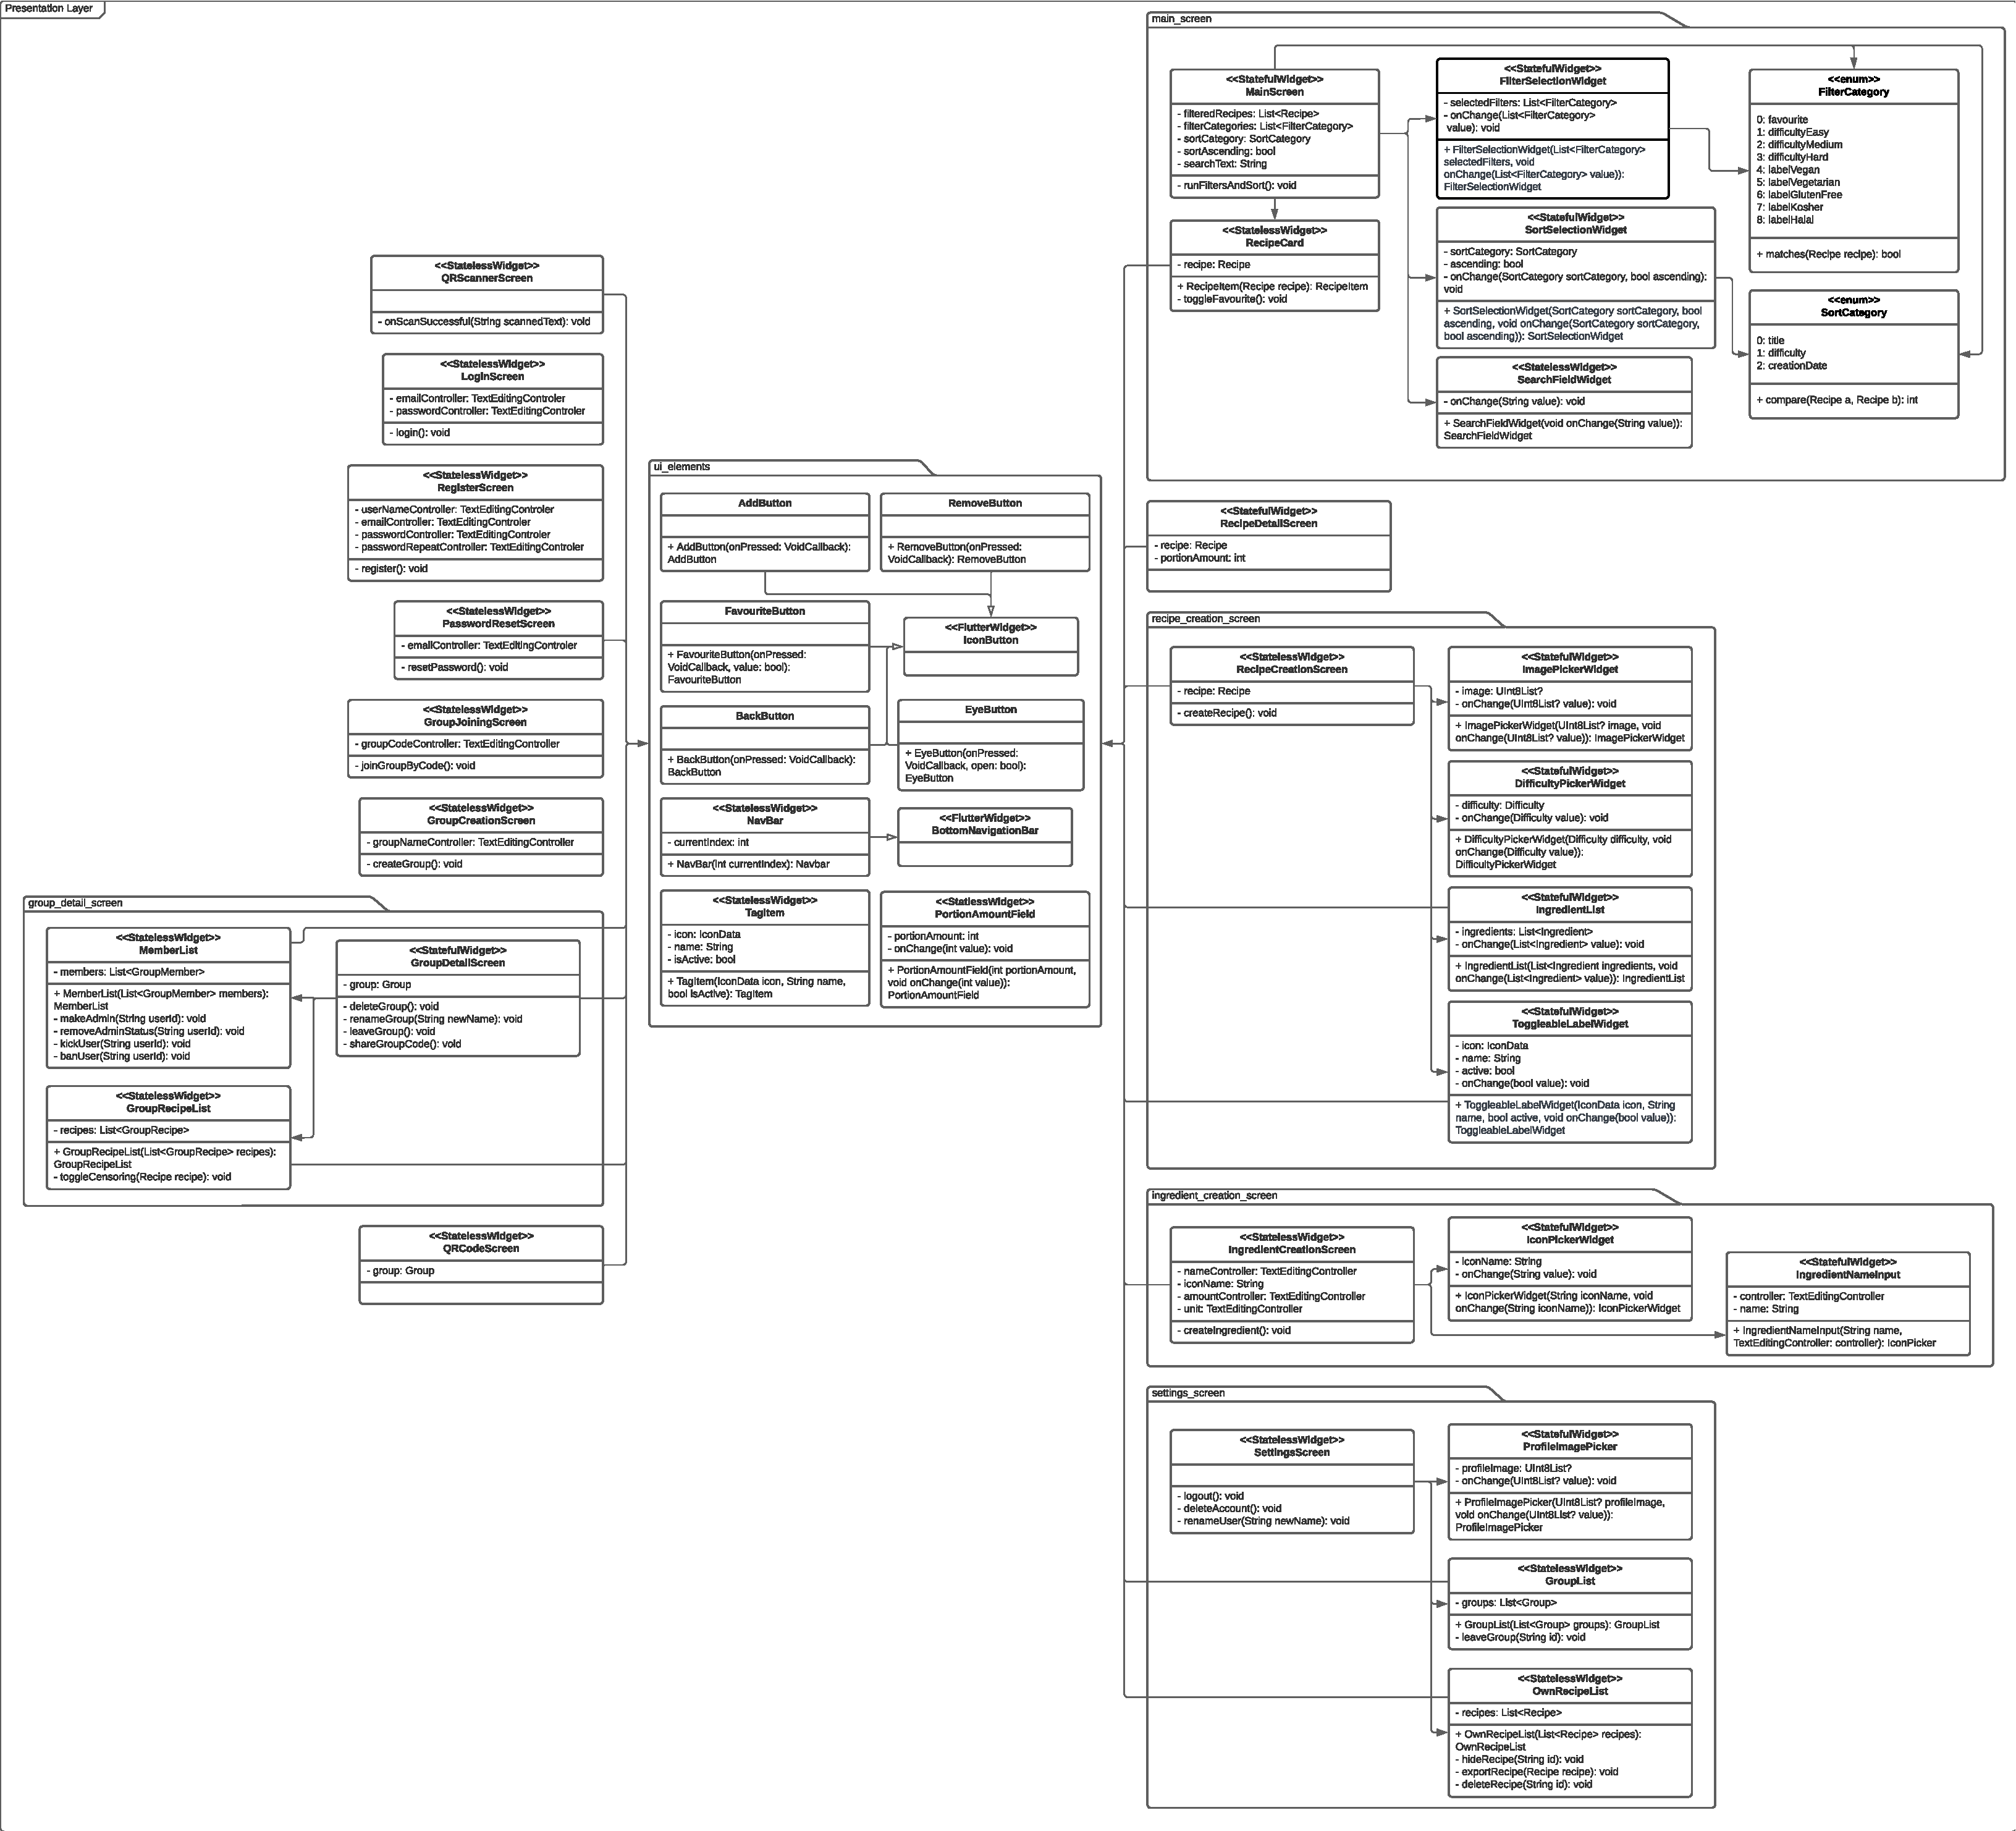
\includegraphics[width = \textwidth]{images/presentationLayer/classDiagrams/presentationLayer.pdf}
    \caption{Klassendiagramm des Presentation Layer}
    \label{fig:presentation-layer}
\end{figure}
\newpage

\subsection{Allgemeine Widgets}
Eigene Widgets, die in mehreren Klassen verwendet werden, werden in einem eigenen Package \texttt{ui\_elements} gespeichert. Diese sollen nun beschrieben werden.
\begin{figure}[htp]
    \centering
    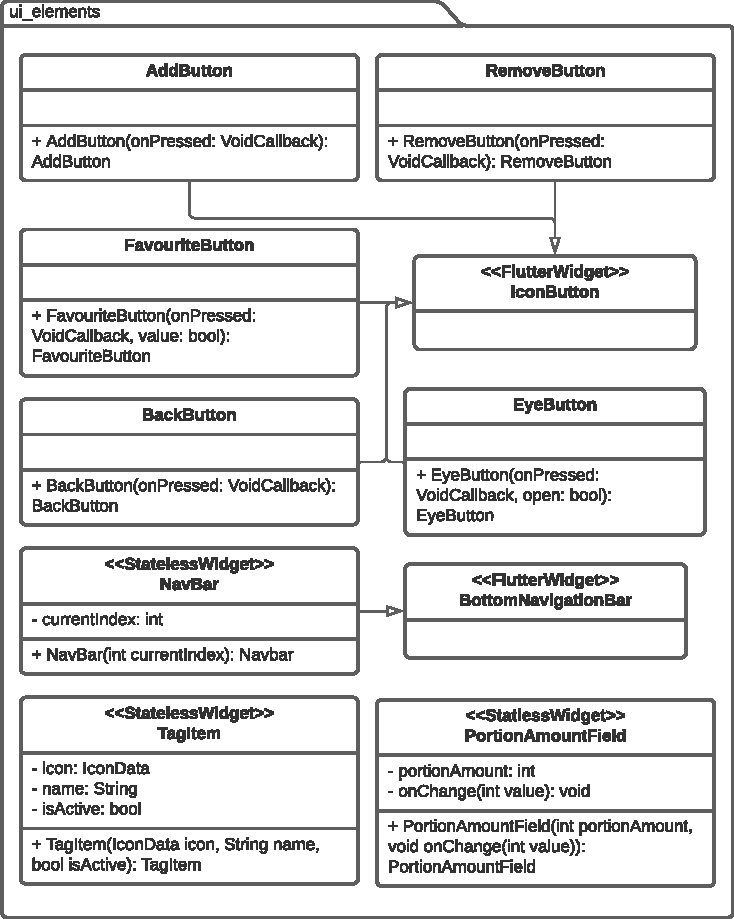
\includegraphics[height = .5\textheight]{images/presentationLayer/classDiagrams/uiElementsWhole.pdf}
    \caption{Klassendiagramm des ui\_elements-Packages}
    \label{fig:ui-elements}
\end{figure}

\subsubsection{\texttt{AddButton}}
\label{sec:addButton}
Der \texttt{AddButton} ist ein Button, der ein Plus-Symbol enthält. Er wird verwendet, um ein neues Element hinzuzufügen. Er erbt von der Flutter-Klasse \texttt{IconButton}.
\begin{figure}[htp]
    \centering
    
\includegraphics[height = .5cm]{images/presentationLayer/uiElements/addButton.png}
    \caption{Darstellung des AddButtons}
\end{figure}
\paragraph*{Konstruktor}
Der Konstruktor nimmt eine Funktion \texttt{onPressed} entgegen, die ausgeführt wird, wenn der Button gedrückt wird.

\subsubsection{\texttt{RemoveButton}}
\label{sec:removeButton}
Der \texttt{RemoveButton} ist ein Button, der ein Kreuz-Symbol enthält. Er wird verwendet, um ein Element zu entfernen. Er erbt von der Flutter-Klasse \texttt{IconButton}.
\begin{figure}[htp]
    \centering
    
\includegraphics[height = .5cm]{images/presentationLayer/uiElements/removeButton.png}
    \caption{Darstellung des RemoveButtons}
\end{figure}
\paragraph*{Konstruktor}
Der Konstruktor nimmt eine Funktion \texttt{onPressed} entgegen, die ausgeführt wird, wenn der Button gedrückt wird.

\subsubsection{\texttt{FavouriteButton}}
\label{sec:favouriteButton}
Der \texttt{FavouriteButton} ist ein Button, der ein Herz-Symbol enthält. Er wird verwendet, um ein Element zu den Favoriten hinzuzufügen. Er erbt von der Flutter-Klasse \texttt{IconButton} und ist je nach übergebenem Wert ausgefüllt oder leer.
\begin{figure}[htp]
    \centering
    
\includegraphics[height = .5cm]{images/presentationLayer/uiElements/favouriteButton.png}
    \caption{Darstellung des FavouriteButtons im gefüllten Zustand}
\end{figure}
\paragraph*{Konstruktor}
Der Konstruktor nimmt eine Funktion \texttt{onPressed} entgegen, die ausgeführt wird, wenn der Button gedrückt wird. Zudem kann ein Boolean \texttt{value} übergeben werden, der bestimmt, ob der Button gefüllt oder leer ist.

\subsubsection{\texttt{EyeButton}}
\label{sec:eyeButton}
Der \texttt{EyeButton} ist ein Button, der ein Augen-Symbol enthält. Er wird verwendet, um ein Element aus- oder einzublenden. Er erbt von der Flutter-Klasse \texttt{IconButton} und das Auge ist je nach übergebenem Wert offen oder geschlossen.
\begin{figure}[htp]
    \centering
    
\includegraphics[height = .5cm]{images/presentationLayer/uiElements/eyeButton.png}
    \caption{Darstellung des EyeButtons im offenen Zustand}
\end{figure}
\paragraph*{Konstruktor}
Der Konstruktor nimmt eine Funktion \texttt{onPressed} entgegen, die ausgeführt wird, wenn der Button gedrückt wird. Zudem kann ein Boolean \texttt{open} übergeben werden, der bestimmt, ob der Button offen oder geschlossen ist.
\newpage

\subsubsection{\texttt{BackButton}}
\label{sec:backButton}
Der \texttt{BackButton} ist ein Button, der ein Pfeil-Symbol enthält. Er wird verwendet, um zur vorherigen Ansicht zurückzukehren. Er erbt von der Flutter-Klasse \texttt{IconButton}.
\begin{figure}[htp]
    \centering
    
\includegraphics[height = 1cm]{images/presentationLayer/uiElements/backButton.png}
    \caption{Darstellung des BackButtons}
\end{figure}
\paragraph*{Konstruktor}
Der Konstruktor nimmt eine Funktion \texttt{onPressed} entgegen, die ausgeführt wird, wenn der Button gedrückt wird.

\subsubsection{\texttt{TagItem}}
\label{sec:tagItem}
Das \texttt{TagItem} ist ein Widget, das ein Symbol und Text enthält. Er wird verwendet, um z.B. Label eines Rezepts zu repräsentieren. Es handelt sich um ein \texttt{StatelessWidget}, da es keinen eigenen Zustand besitzt.
\begin{figure}[htp]
    \centering
    
\includegraphics[height = .7cm]{images/presentationLayer/uiElements/tagItem.png}
    \caption{Darstellung eines TagItems}
\end{figure}
\paragraph*{Konstruktor}
Der Konstruktor nimmt einen String \texttt{text} entgegen, der den Text des Widgets bestimmt. Zudem muss ein IconData \texttt{icon} übergeben werden, der das Symbol des Widgets bestimmt.

\subsubsection{\texttt{PortionAmountField}}
\label{sec:portionAmountField}
Das \texttt{PortionAmountField} ist ein Textfeld, das verwendet wird, um die Anzahl der Portionen anzugeben. Es handelt sich um ein \texttt{StatelessWidget}, da es keinen eigenen Zustand besitzt.
\begin{figure}[htp]
    \centering
    
\includegraphics[height = 1cm]{images/presentationLayer/uiElements/portionAmountField.png}
    \caption{Darstellung eines PortionAmountFields}
\end{figure}
\paragraph*{Konstruktor}
Der Konstruktor nimmt eine Funktion \texttt{onChange} entgegen, die ausgeführt wird, wenn sich der Text im Textfeld ändert. Zudem muss ein Integer \texttt{portionAmount} übergeben werden, der den initialen Wert des Textfelds bestimmt.

\subsubsection{\texttt{NavBar}}
\label{sec:navBar}
Die \texttt{NavBar} ist eine Navigationsleiste, die am unteren Rand der App angezeigt wird. Sie erbt von der Flutter-Klasse \texttt{BottomNavigationBar}. Es kann zur Rezept-Erstellungs-Ansicht, zur Hauptansicht und zur Einstellungsansicht navigiert werden.
\begin{figure}[htp]
    \centering
    
\includegraphics[height = 1.5cm]{images/presentationLayer/uiElements/navBar.png}
    \caption{Darstellung der NavBar}
\end{figure}
\newpage

\subsection{\texttt{LoginScreen}}
\label{sec:loginScreen}
Die Klasse bildet die Loginansicht ab. Die Klasse \texttt{LoginScreen} ist ein \texttt{StatelessWidget}, da sie keinen eigenen Zustand besitzt.
\begin{figure}[htp]
    \begin{minipage}
        [t]{0.49\textwidth}
        \centering
        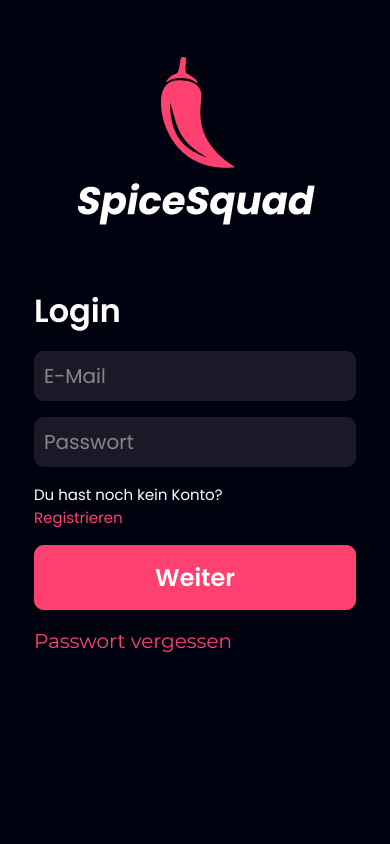
\includegraphics[height=80mm]{images/presentationLayer/uiElements/loginScreen.jpg}
        \caption{Loginansicht}
    \end{minipage}
    \begin{minipage}
        [t]{0.49\textwidth}
        \centering
        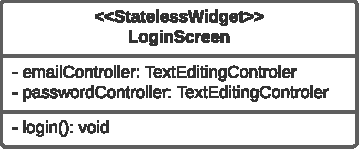
\includegraphics[width=0.95\textwidth]{images/presentationLayer/classDiagrams/loginScreen.pdf}
        \caption{Klassendiagramm des Login\-Screens}
    \end{minipage}
\end{figure}
\subsubsection*{Attribute}
\paragraph{\texttt{emailController: TextEditingController}}
Der Controller, der die Eingabe der E-Mail-Ad\-resse des Nutzers verwaltet. Über ihn kann der Wert des Eingabefelds abgerufen werden oder eine Fehlermeldung angezeigt werden.
\paragraph{\texttt{passwordController: TextEditingController}}
Der Controller, der die Eingabe des Passworts des Nutzers verwaltet. Über ihn kann der Wert des Eingabefelds abgerufen werden oder eine Fehlermeldung angezeigt werden.
\subsubsection*{Methoden}
\paragraph{\texttt{login(): void}}
Leitet eine Loginanfrage über einen Provider an den zuständigen Service weiter. Im Anschluss werden, jenachdem ob die Anfrage erfolgreich war oder nicht, Fehlermeldungen an den entsprechenden Eingabefeldern angezeigt, oder der Nutzer zur Hauptansicht (\ref{sec:mainScreen}) weitergeleitet.

\newpage
\subsection{\texttt{RegisterScreen}}
\label{sec:registerScreen}
Die Klasse bildet die Registrierungsansicht ab. Sie ist ein \texttt{StatelessWidget}, da sie keinen eigenen Zustand besitzt.
\begin{figure}[htp]
    \begin{minipage}
        [t]{0.49\textwidth}
        \centering
        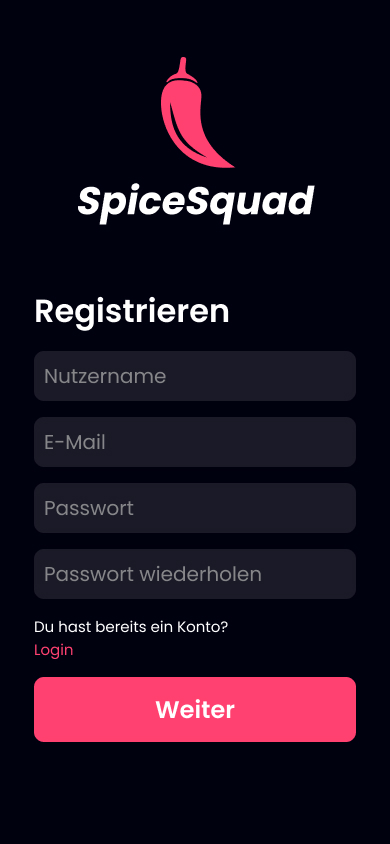
\includegraphics[height=80mm]{images/presentationLayer/uiElements/registerScreen.jpg}
        \caption{Registrierungsansicht}
    \end{minipage}
    \begin{minipage}
        [t]{0.49\textwidth}
        \centering
        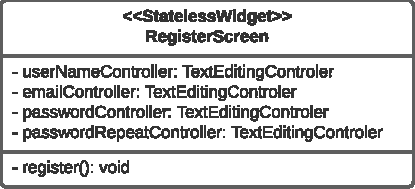
\includegraphics[width=0.95\textwidth]{images/presentationLayer/classDiagrams/registerScreen.pdf}
        \caption{\protect\raggedright Klassendiagramm des Register\-Screens}
    \end{minipage}
\end{figure}
\subsubsection*{Attribute}
\paragraph{\texttt{userNameController: TextEditingController}}
Der Controller, der die Eingabe des Benutzernamens des Nutzers verwaltet. Über ihn kann der Wert des Eingabefelds abgerufen werden oder eine Fehlermeldung angezeigt werden.
\paragraph{\texttt{emailController: TextEditingController}}
Der Controller, der die Eingabe der E-Mail-Ad\-resse des Nutzers verwaltet. Über ihn kann der Wert des Eingabefelds abgerufen werden oder eine Fehlermeldung angezeigt werden.
\paragraph{\texttt{passwordController: TextEditingController}}
Der Controller, der die Eingabe des Passworts des Nutzers verwaltet. Über ihn kann der Wert des Eingabefelds abgerufen werden oder eine Fehlermeldung angezeigt werden.
\paragraph{\texttt{passwordRepeatController: TextEditingController}}
Der Controller, der die Eingabe der Passwortwiederholung des Nutzers verwaltet. Über ihn kann der Wert des Eingabefelds abgerufen werden oder eine Fehlermeldung angezeigt werden.
\subsubsection*{Methoden}
\paragraph{\texttt{register(): void}}
Leitet eine Registrierungsanfrage über einen Provider an den zuständigen Service weiter. Im Anschluss werden, jenachdem ob die Anfrage erfolgreich war oder nicht, Fehlermeldungen an den entsprechenden Eingabefeldern angezeigt, oder der Nutzer zur Gruppen-Beitritts-Ansicht (\ref{sec:groupJoiningScreen}) weitergeleitet.
\newpage

\subsection{\texttt{PasswordResetScreen}}
\label{sec:passwordResetScreen}
Die Klasse bildet die Passwort-Zurücksetzen-Ansicht ab. Sie ist ein \texttt{StatelessWidget}, da sie keinen eigenen Zustand besitzt. Sie verwendet die Klasse \nameref{sec:backButton} aus dem \texttt{ui\_elements}-Package.
\begin{figure}[htp]
    \begin{minipage}
        [t]{0.49\textwidth}
        \centering
        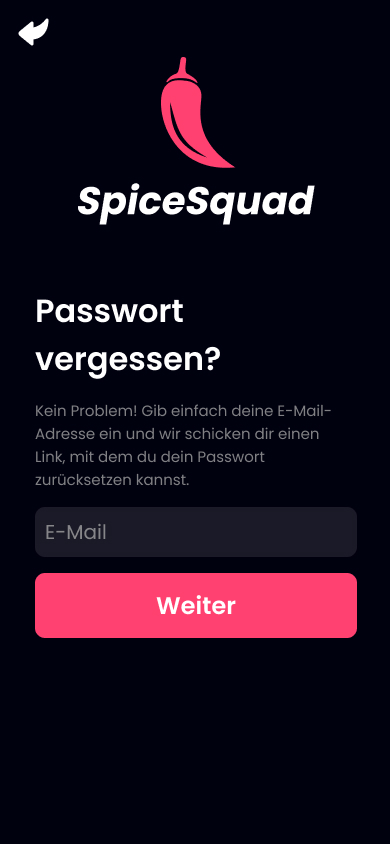
\includegraphics[height=80mm]{images/presentationLayer/uiElements/passwordResetScreen.jpg}
        \caption{Passwort-Zurücksetzen-Ansicht}
    \end{minipage}
    \begin{minipage}
        [t]{0.49\textwidth}
        \centering
        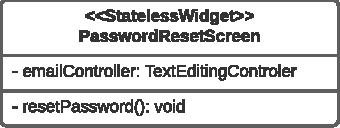
\includegraphics[width=0.95\textwidth]{images/presentationLayer/classDiagrams/passwordResetScreen.pdf}
        \caption{\protect\raggedright Klassendiagramm des Password\-Reset\-Screens}
    \end{minipage}
\end{figure}

\subsubsection*{Attribute}
\paragraph{\texttt{emailController: TextEditingController}}
Der Controller, der die Eingabe der E-Mail-Ad\-resse des Nutzers verwaltet. Über ihn kann der Wert des Eingabefelds abgerufen werden oder eine Fehlermeldung angezeigt werden.

\subsubsection*{Methoden}
\paragraph{\texttt{resetPassword(): void}}
Leitet eine Registrierungsanfrage über einen Provider an den zuständigen Service weiter. Zeigt bei Erfolg einen \Gls{Dialog} an, dass die Anfrage erfolgreich war. Im Anschluss wird der Nutzer zur Anmeldeansicht (\ref{sec:loginScreen}) weitergeleitet.
\newpage

\subsection{\texttt{GroupJoiningScreen}}
\label{sec:groupJoiningScreen}
Die Klasse bildet die Gruppen-Beitritts-Ansicht ab. Sie ist ein \texttt{StatelessWidget}, da sie keinen eigenen Zustand besitzt.
Befindet sich die Registrierungsansicht (\ref{sec:registerScreen}) im Navigations-Stack, wird ein Überspringen-Knopf angezeigt, der zur Hauptansicht (\ref{sec:mainScreen}) führt.
Drückt der Nutzer auf den Knopf "Mit QR-Code beitreten" wird er zur QR-Code-Scan-Ansicht (\ref{sec:qrScannerScreen}) weitergeleitet. Gibt die Ansicht einen String zurück, wird eine Gruppenbeitrittsanfrage über einen Provider an den zuständigen Service weitergeleitet. Im Anschluss wird der Nutzer, jenachdem ob der Nutzer von der Registrierungsansicht (\ref{sec:registerScreen}) kommt oder nicht, zur Hauptansicht (\ref{sec:mainScreen}) oder zur vorherigen Ansicht weitergeleitet.
\begin{figure}[htp]
    \begin{minipage}
        [t]{0.49\textwidth}
        \centering
        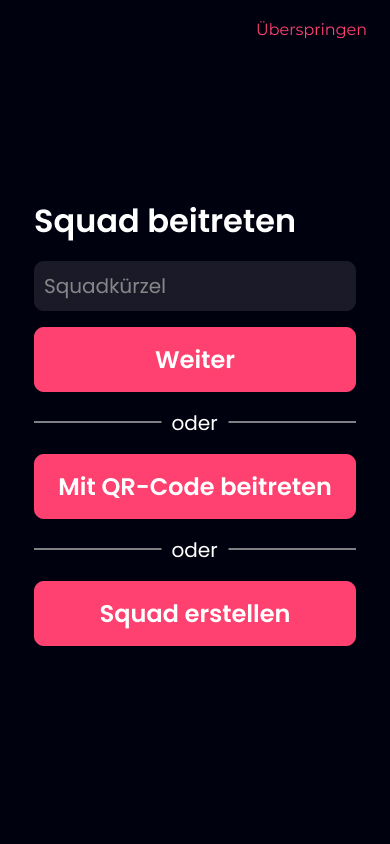
\includegraphics[height=80mm]{images/presentationLayer/uiElements/groupJoiningScreen.jpg}
        \caption{Gruppen-Beitritts-Ansicht}
    \end{minipage}
    \begin{minipage}
        [t]{0.49\textwidth}
        \centering
        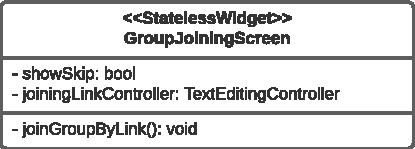
\includegraphics[width=0.95\textwidth]{images/presentationLayer/classDiagrams/groupJoiningScreen.pdf}
        \caption{\protect\raggedright Klassendiagramm des Group\-Joining\-Screens}
    \end{minipage}
\end{figure}
\subsubsection*{Attribute}
\paragraph{\texttt{groupCodeController: TextEditingController}}
Der Controller, der die Eingabe des Gruppencodes des Nutzers verwaltet. Über ihn kann der Wert des Eingabefelds abgerufen werden oder eine Fehlermeldung angezeigt werden.
\subsubsection*{Methoden}
\paragraph{\texttt{joinGroupByCode(): void}}
Leitet eine Gruppenbeitrittsanfrage über einen Provider an den zuständigen Service weiter, wobei das Gruppenkürzel übergegeben wird. Zeigt bei Erfolg einen \Gls{Dialog} an, dass die Anfrage erfolgreich war. Im Anschluss wird der Nutzer entweder zur Hauptansicht (\ref{sec:mainScreen}) oder zur vorherigen Ansicht weitergeleitet. Dies hängt davon ab, ob die Registrierungsansicht (\ref{sec:registerScreen}) im Navigations-Stack ist.
\newpage

\subsection{\texttt{QRScannerScreen}}
\label{sec:qrScannerScreen}
Die Klasse bildet die QR-Scanner-Ansicht ab. Sie ist ein \texttt{StatelessWidget}, da sie keinen eigenen Zustand besitzt. Sie verwendet die Klasse \nameref{sec:backButton} aus dem \texttt{ui\_elements}-Package. Es handelt sich um eine Ansicht, die die Kameraansicht des Smartphones zeigt.
\begin{figure}
    [htp]
    \centering
    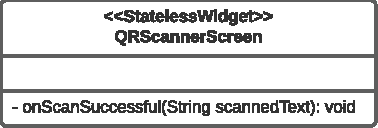
\includegraphics[width=.49\textwidth]{images/presentationLayer/classDiagrams/qrScannerScreen.pdf}
    \caption{Klassendiagramm des QR\-Scanner\-Screens}
\end{figure}
\subsubsection*{Methoden}
\paragraph{\texttt{onScanSuccessful(String scannedText): void}}
Wird ein QR-Code erkannt, so wird diese Methode mit dem entschlüsselten Text aufgerufen. Sie validiert, ob es sich um ein Gruppenkürzel handelt und gibt es bei Erfolg an die vorherige Ansicht zurück. Die Erkennung des QR-Codes erfolgt über das Flutter-Package \texttt{mobile\_scanner}.

\newpage
\subsection{\texttt{GroupCreationScreen}}
\label{sec:groupCreationScreen}
Die Klasse bildet die Gruppen-Erstellungs-Ansicht ab. Sie ist ein \texttt{StatelessWidget}, da sie keinen eigenen Zustand besitzt.
Befindet sich die Registrierungsansicht (\ref{sec:registerScreen}) im Navigations-Stack, wird ein Überspringen-Knopf angezeigt, der zur Hauptansicht (\ref{sec:mainScreen}) führt.
\begin{figure}[htp]
    \begin{minipage}
        [t]{0.49\textwidth}
        \centering
        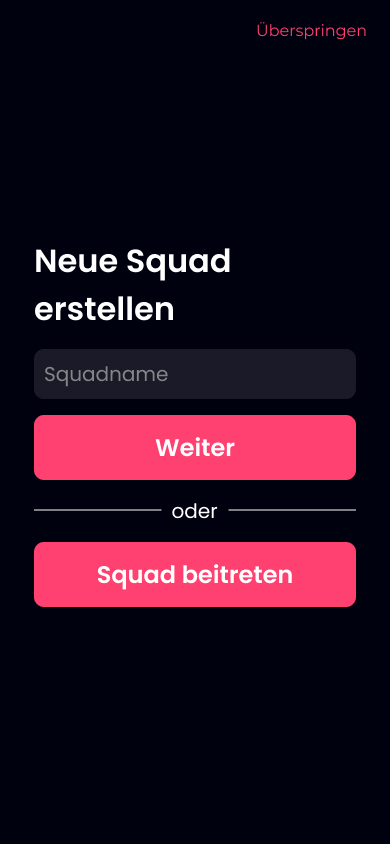
\includegraphics[height=80mm]{images/presentationLayer/uiElements/groupCreationScreen.jpg}
        \caption{Gruppen-Erstellungs-Ansicht}
    \end{minipage}
    \begin{minipage}
        [t]{0.49\textwidth}
        \centering
        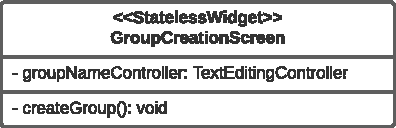
\includegraphics[width=0.95\textwidth]{images/presentationLayer/classDiagrams/groupCreationScreen.pdf}
        \caption{\protect\raggedright Klassendiagramm des Group\-Creation\-Screens}
    \end{minipage}
\end{figure}
\subsubsection*{Attribute}
\paragraph{\texttt{groupNameController: TextEditingController}}
Der Controller, der die Eingabe des Gruppennamens durch den Nutzer verwaltet. Über ihn kann der Wert des Eingabefelds abgerufen werden oder eine Fehlermeldung angezeigt werden.
\subsubsection*{Methoden}
\paragraph{\texttt{createGroup(): void}}
Leitet eine Gruppenerstellungsanfrage über einen Provider an den zuständigen Service weiter, wobei der Gruppenname übergeben wird. Zeigt bei Erfolg einen \Gls{Dialog} an, dass die Anfrage erfolgreich war. Im Anschluss wird der Nutzer entweder zur Hauptansicht (\ref{sec:mainScreen}) oder zur vorherigen Ansicht weitergeleitet. Dies hängt davon ab, ob die Registrierungsansicht (\ref{sec:registerScreen}) im Navigations-Stack ist.
\newpage

\subsection{\texttt{main\_screen}}
Das Package \texttt{main\_screen} enthält alle Klassen für die Hauptansicht der App. Der anzuzeigende Screen ist in der Klasse \hyperref[sec:mainScreen]{\texttt{MainScreen}} implementiert
\begin{figure}
    [htp]
    \centering
    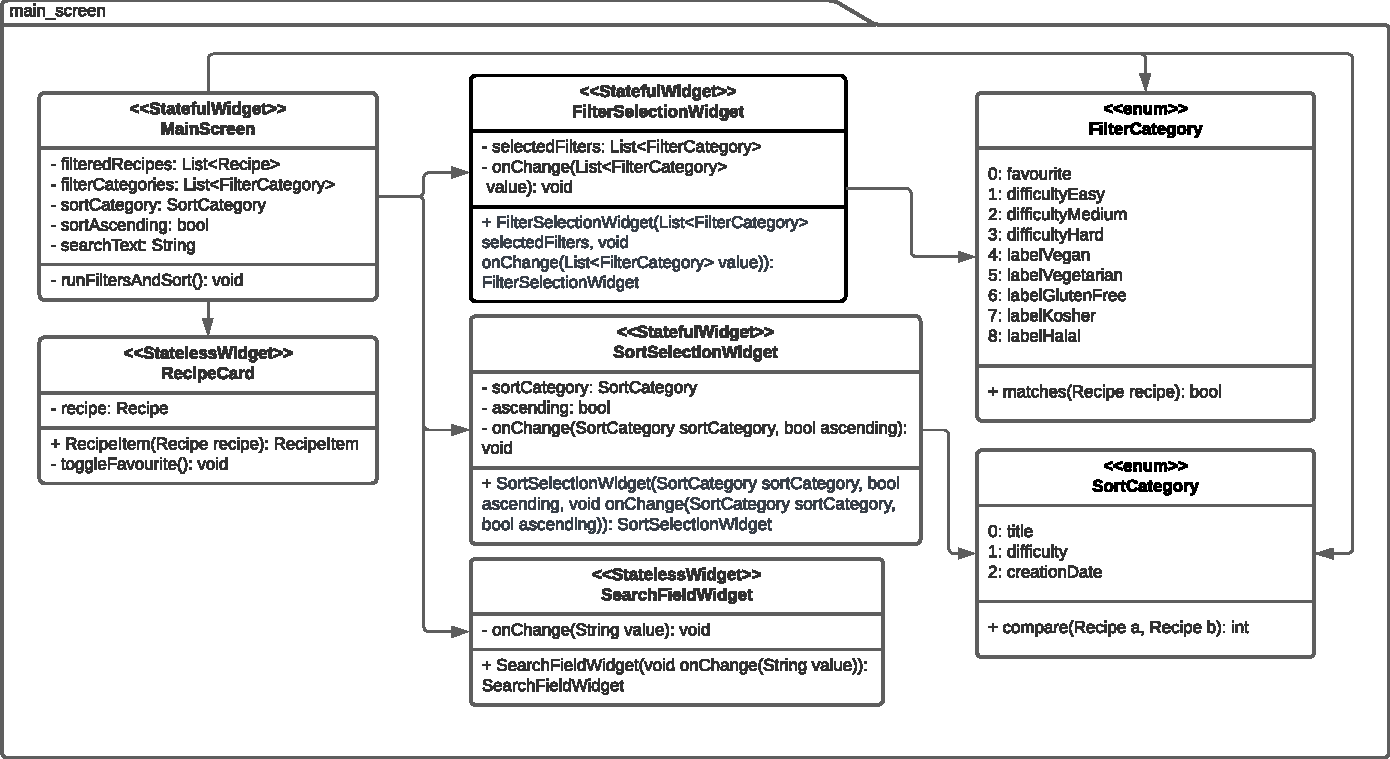
\includegraphics[width=\textwidth]{images/presentationLayer/classDiagrams/mainScreenWhole.pdf}
    \caption{Klassendiagramm des Pakets main\_screen}
\end{figure}
\newpage
\subsubsection{\texttt{MainScreen}}
\label{sec:mainScreen}
Die Klasse bildet die Hauptansicht der App ab. Sie ist ein \texttt{StatefulWidget}, da sie den Zustand \texttt{filteredRecipes} verwaltet und anzeigt. Sie bildet für jedes Rezept eine \texttt{RecipeCard} ab. Zudem gibt es zwei Widgets zur Auswahl der Sortierung und Filterung der Rezepte und eines zum Suchen.
\begin{figure}[htp]
    \begin{minipage}
        [t]{0.49\textwidth}
        \centering
        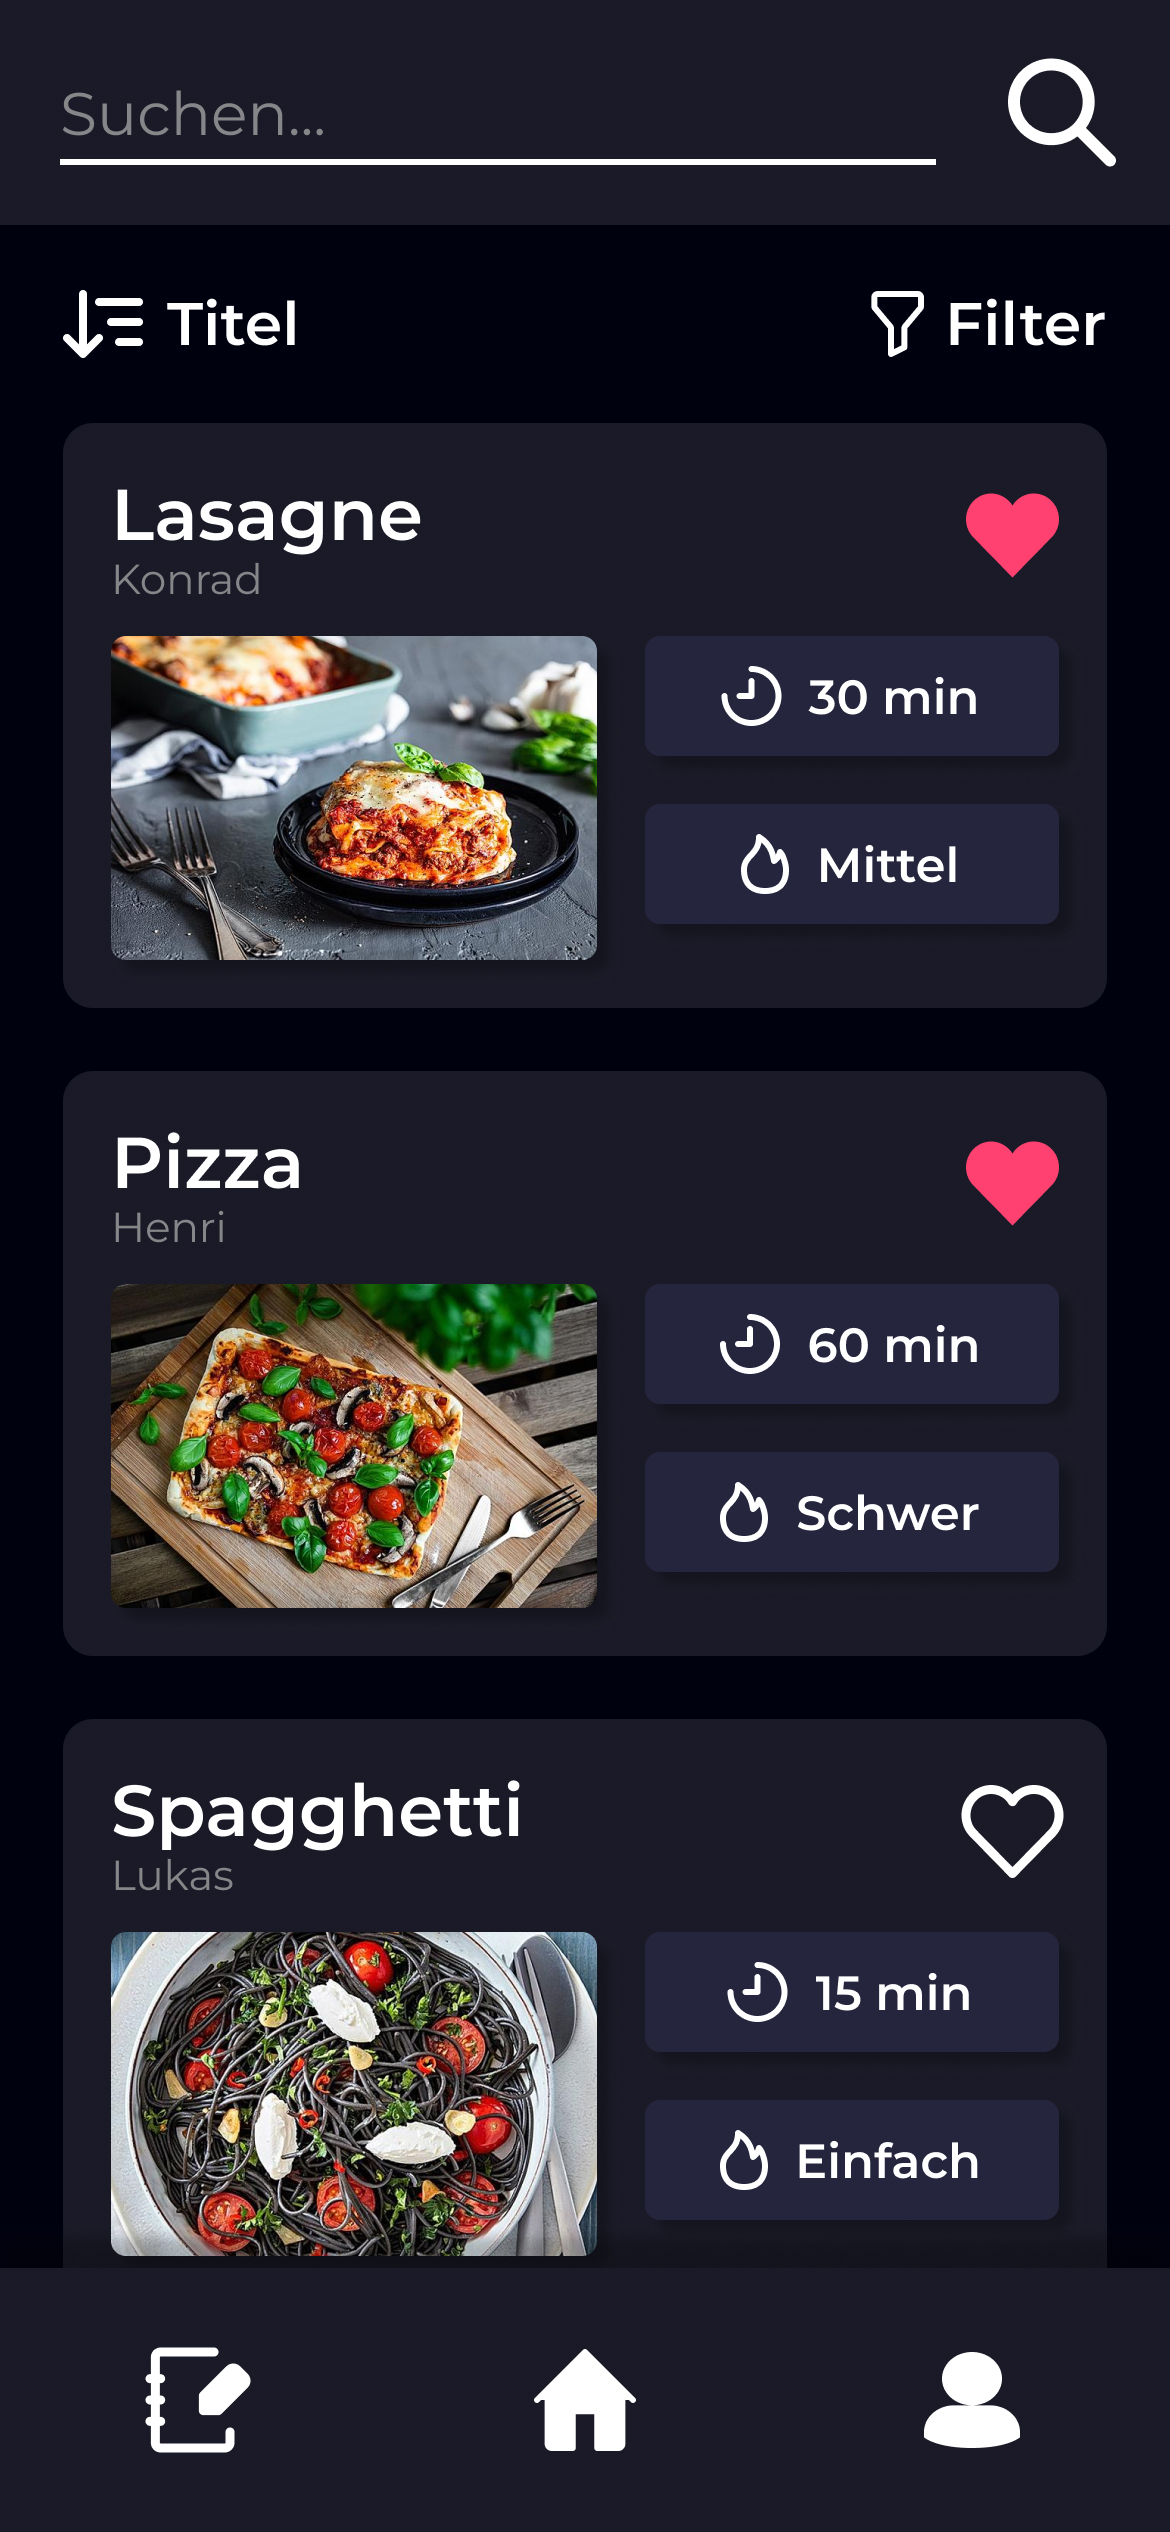
\includegraphics[height=80mm]{images/presentationLayer/uiElements/mainScreen.jpg}
        \caption{Hauptansicht der App}
    \end{minipage}
    \begin{minipage}
        [t]{0.49\textwidth}
        \centering
        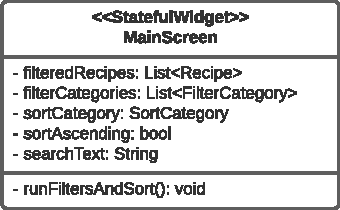
\includegraphics[width=0.95\textwidth]{images/presentationLayer/classDiagrams/mainScreen.pdf}
        \caption{\protect\raggedright Klassendiagramm des Main\-Screens}
    \end{minipage}
\end{figure}
\subsubsection*{Attribute}
\paragraph{\texttt{filteredRecipes: List<Recipe>}}
Die Liste der Rezepte, die aktuell angezeigt werden. Sie wird durch die Auswahl der Sortierung und Filterung bestimmt.
\paragraph{\texttt{filterCategories: List<FilterCategory}}
Die Liste der Filterkategorien, die aktuell ausgewählt sind.
\paragraph{\texttt{sortCategory: SortCategory}}
Die aktuell ausgewählte Sortierung.
\paragraph{\texttt{sortAscending: bool}}
Gibt an, ob die Sortierung aufsteigend ist.
\paragraph{\texttt{searchText: String}}
Der aktuell eingegebene Suchtext.
\subsubsection*{Methoden}
\paragraph{\texttt{runFiltersAndSort(): void}}
Wendet die aktuell ausgewählten Filter, die Suche und die Sortierung auf die Liste aller Rezepte an und speichert das Ergebnis in \texttt{filteredRecipes}. Wird immer aufgerufen, nachdem sich eine der Einstellungen geändert hat.
\newpage
\subsubsection{\texttt{RecipeCard}}
\label{sec:recipeCard}
Die Klasse bildet eine Rezeptkarte ab. Sie ist ein \texttt{StatelessWidget}, da sie keinen eigenen Zustand besitzt. Sie verwendet die Klasse \nameref{sec:favouriteButton} aus dem Package \texttt{ui\_elements}.
\begin{figure}[htp]
    \begin{minipage}
        [t]{0.49\textwidth}
        \centering
        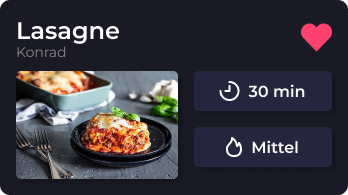
\includegraphics[width=.8\textwidth]{images/presentationLayer/uiElements/recipeCard.png}
        \caption{Abbildung einer Rezeptkarte}
    \end{minipage}
    \begin{minipage}
        [t]{0.49\textwidth}
        \centering
        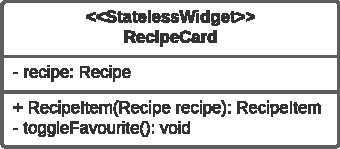
\includegraphics[width=0.95\textwidth]{images/presentationLayer/classDiagrams/recipeCard.pdf}
        \caption{\protect\raggedright Klassendiagramm der Recipe\-Card}
    \end{minipage}
\end{figure}
\subsubsection*{Attribute}
\paragraph{\texttt{recipe: Recipe}}
Das Rezept, das angezeigt werden soll.
\subsubsection*{Methoden}
\paragraph{\texttt{RecipeItem(Recipe recipe): RecipeItem}}
Konstruktor, der das anzuzeigende Rezept übergeben bekommt.
\paragraph{\texttt{toggleFavourite(): void}}
Leitet eine Anfrage über den zugehörigen Provider an den zuständigen Service weiter, um das Rezept als Favorit zu markieren oder die Markierung aufzuheben.
\newpage
\subsubsection{\texttt{FilterSelectionWidget}}
\label{sec:filterSelectionWidget}
Die Klasse stellt ein Widget bereit, mit dem der Nutzer die Filterkategorien auswählen kann. Sie ist ein \texttt{StatefulWidget}, da sie den Zustand \texttt{selectedCategories} verwaltet. Wird auf das Widget gedrückt, öffnet sich ein \Gls{Dialog}, in dem die Filterkategorien ausgewählt werden können.
\begin{figure}[htp]
    \begin{minipage}
        [t]{0.49\textwidth}
        \centering
        
\includegraphics[width=1.5cm]{images/presentationLayer/uiElements/filterSelectionWidget.png}
        \caption{\protect\raggedright Abbildung des Filter\-Selection\-Widgets}
    \end{minipage}
    \begin{minipage}
        [t]{0.49\textwidth}
        \centering
        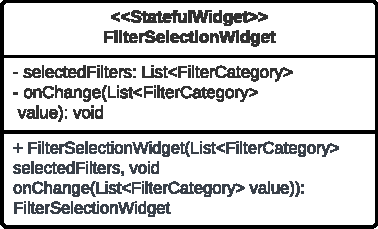
\includegraphics[width=0.95\textwidth]{images/presentationLayer/classDiagrams/filterSelectionWidget.pdf}
        \caption{\protect\raggedright Klassendiagramm des Filter\-Selection\-Widgets}
    \end{minipage}
\end{figure}
\subsubsection*{Attribute}
\paragraph{\texttt{selectedFilters: List<FilterCategory>}}
Die Liste der aktuell ausgewählten Filterkategorien.
\paragraph{\texttt{onChange(List<FilterCategory> value): void}} Callback-Methode, die ausgeführt wird wenn sich die Auswahl der Filterkategorien ändert und die neue Auswahl als Parameter übergeben bekommt.
\subsubsection*{Methoden}
\paragraph{\texttt{FilterSelectionWidget(List<FilterCategory> selectedFilters, void onChange(List<FilterCategory> value)): FilterSelectionWidget}}
Konstruktor, der die aktuell ausgewählten Filterkategorien und die Callback-Methode übergeben bekommt.
\newpage

\subsubsection{\texttt{FilterCategory}}
\label{sec:filterCategory}
\begin{figure}
    [htp]
    \centering
    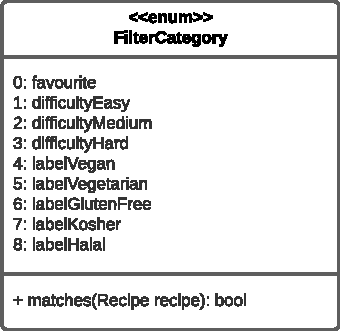
\includegraphics[width=0.3\textwidth]{images/presentationLayer/classDiagrams/filterCategory.pdf}
    \caption{Klassendiagramm des Enums Filter\-Category}
\end{figure}
Der Enum \texttt{FilterCategory} bildet die Filterkategorien ab. Die Kategorien sind:
\begin{itemize}
    \item \texttt{favourite}
    \item \texttt{difficultyEasy}
    \item \texttt{difficultyMedium}
    \item \texttt{difficultyHard}
    \item \texttt{labelVegan}
    \item \texttt{labelVegetarian}
    \item \texttt{labelGlutenFree}
    \item \texttt{labelKosher}
    \item \texttt{labelHalal}
\end{itemize}
\subsubsection*{Methoden}
\paragraph{\texttt{matches(Recipe recipe): bool}}
Gibt an, ob das übergebene Rezept zu der Filterkategorie passt. Kann zum Filtern einer Rezeptliste benutzt werden.
\newpage

\subsubsection{\texttt{SortSelectionWidget}}
\label{sec:sortSelectionWidget}
Die Klasse stellt ein Widget bereit, mit dem der Nutzer die Sortierung auswählen kann. Sie ist ein \texttt{StatefulWidget}, da sie die Zustände \texttt{sortCategory} und \texttt{ascending} verwaltet. Wird auf das Widget gedrückt, öffnet sich ein \Gls{Dialog}, in dem die Sortierung ausgewählt werden kann.

\begin{figure}[htp]
    \begin{minipage}
        [t]{0.49\textwidth}
        \centering
        
\includegraphics[width=1.5cm]{images/presentationLayer/uiElements/sortSelectionWidget.png}
        \caption{\protect\raggedright Abbildung des Sort\-Selection\-Widgets}
    \end{minipage}
    \begin{minipage}
        [t]{0.49\textwidth}
        \centering
        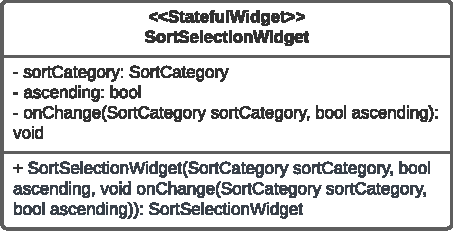
\includegraphics[width=0.95\textwidth]{images/presentationLayer/classDiagrams/sortSelectionWidget.pdf}
        \caption{\protect\raggedright Klassendiagramm des Sort\-Selection\-Widgets}
    \end{minipage}
\end{figure}

\subsubsection*{Attribute}
\paragraph{\texttt{sortCategory: SortCategory}}
Die aktuell ausgewählte Sortierungskategorie.
\paragraph{\texttt{ascending: bool}}
Gibt an, ob die Sortierung aufsteigend sein soll.
\paragraph{\texttt{onChange(SortCategory sortCategory, bool ascending): void}} Callback-Methode, die ausgeführt wird wenn sich die Auswahl der Sortierung ändert und die neue Auswahl als Parameter übergeben bekommt.
\subsubsection*{Methoden}
\paragraph{\texttt{SortSelectionWidget(SortCategory sortCategory, bool ascending, void onChange(SortCategory sortCategory, bool ascending)): SortSelectionWidget}}
Konstruktor, der die aktuell ausgewählte Sortierungskategorie, die Sortierrichtung und die Callback-Methode übergeben bekommt.
\newpage
\subsubsection{\texttt{SortCategory}}
\label{sec:sortCategory}
\begin{figure}
    [htp]
    \centering
    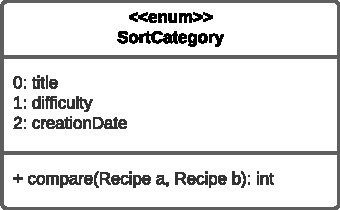
\includegraphics[width=0.3\textwidth]{images/presentationLayer/classDiagrams/sortCategory.pdf}
    \caption{Klassendiagramm des Enums Sort\-Category}
\end{figure}
Der Enum \texttt{SortCategory} bildet die Sortierungskategorien ab. Die Kategorien sind:
\begin{itemize}
    \item \texttt{title}
    \item \texttt{difficulty}
    \item \texttt{creationDate}
\end{itemize}
\subsubsection*{Methoden}
\paragraph{\texttt{compare(Recipe a, Recipe b): int}}
Vergleicht zwei Rezepte anhand der Sortierungskategorie und gibt an, welches Rezept zuerst kommen soll. Kann zum Sortieren einer Rezeptliste mit Hilfe von \texttt{List.sort()} benutzt werden.
\newpage

\subsubsection{\texttt{SearchFieldWidget}}
\label{sec:searchFieldWidget}
Die Klasse stellt ein Widget bereit, mit dem der Nutzer nach Rezepten suchen kann. Sie ist ein \texttt{StatelessWidget}, da sie selbst keinen Zustand verwaltet, der die UI aktualisieren muss. Das übernimmt das zugrundeliegende Textfeld.
\begin{figure}[htp]
    \begin{minipage}
        [t]{0.49\textwidth}
        \centering
        
\includegraphics[width=.95\textwidth]{images/presentationLayer/uiElements/searchFieldWidget.png}
        \caption{\protect\raggedright Abbildung des Search\-Field\-Widgets}
    \end{minipage}
    \begin{minipage}
        [t]{0.49\textwidth}
        \centering
        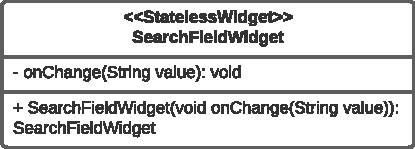
\includegraphics[width=0.95\textwidth]{images/presentationLayer/classDiagrams/searchFieldWidget.pdf}
        \caption{\protect\raggedright Klassendiagramm des Search\-Field\-Widgets}
    \end{minipage}
\end{figure}
\subsubsection*{Attribute}
\paragraph{\texttt{onChange(String value): void}}
Callback-Methode, die ausgeführt wird wenn sich der Inhalt des Textfelds ändert und den neuen Inhalt als Parameter übergeben bekommt.
\subsubsection*{Methoden}
\paragraph{\texttt{SearchFieldWidget(void onChange(String value)): SearchFieldWidget}}
Konstruktor, der die Callback-Methode übergeben bekommt.
\newpage
\subsection{\texttt{RecipeDetailScreen}}
\label{sec:recipeDetailScreen}
Die Klasse stellt den Bildschirm dar, auf dem die Zubereitungsanweisungen eines Rezepts angezeigt werden. Sie ist ein \texttt{StatefulWidget}, da sie den Zustand \texttt{portionAmount} verwaltet. Die Klasse verwendet die Klassen \nameref{sec:backButton}, \nameref{sec:favouriteButton} und \nameref{sec:portionAmountField} aus dem Package \texttt{ui\_elements}. 
\begin{figure}[htp]
    \begin{minipage}
        [t]{0.49\textwidth}
        \centering
        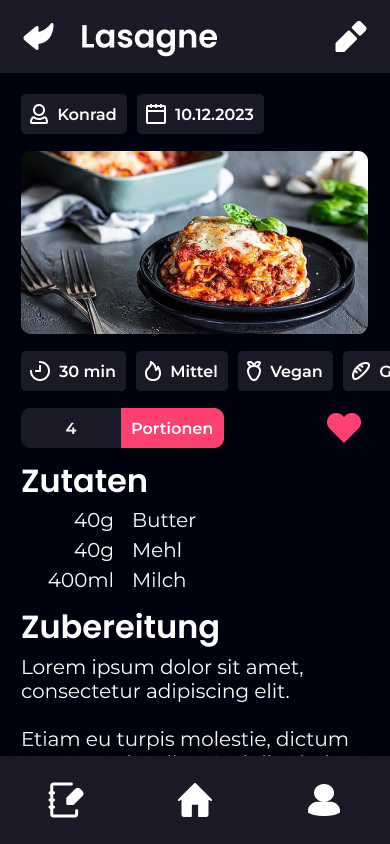
\includegraphics[height=80mm]{images/presentationLayer/uiElements/recipeDetailScreen.jpg}
        \caption{\protect\raggedright Abbildung des Recipe\-Detail\-Screens}
    \end{minipage}
    \begin{minipage}
        [t]{0.49\textwidth}
        \centering
        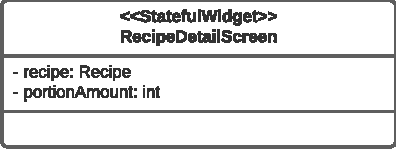
\includegraphics[width=0.95\textwidth]{images/presentationLayer/classDiagrams/recipeDetailScreen.pdf}
        \caption{\protect\raggedright Klassendiagramm des Recipe\-Detail\-Screens}
    \end{minipage}
\end{figure}
\subsubsection*{Attribute}
\paragraph{\texttt{recipe: Recipe}}
Das Rezept, das angezeigt werden soll. Es wird bei der Initialisierung aus dem \Gls{BuildContext} gelesen, wo es vorher hineingeschrieben wurde.
\paragraph{\texttt{portionAmount: int}}
Die Anzahl der Portionen, die der Nutzer kochen möchte. Er kann sie über ein Textfeld setzen, woraufhin die Zutatenmengen angepasst werden.
\newpage

\subsection{\texttt{recipe\_creation\_screen}}
Das Package \texttt{mainrecipe\_creation\_screen} enthält alle Klassen für die Rezept-Erstellungs-Ansicht. Der anzuzeigende Screen ist in der Klasse \nameref{sec:recipeCreationScreen} implementiert.
\begin{figure}
    [htp]
    \centering
    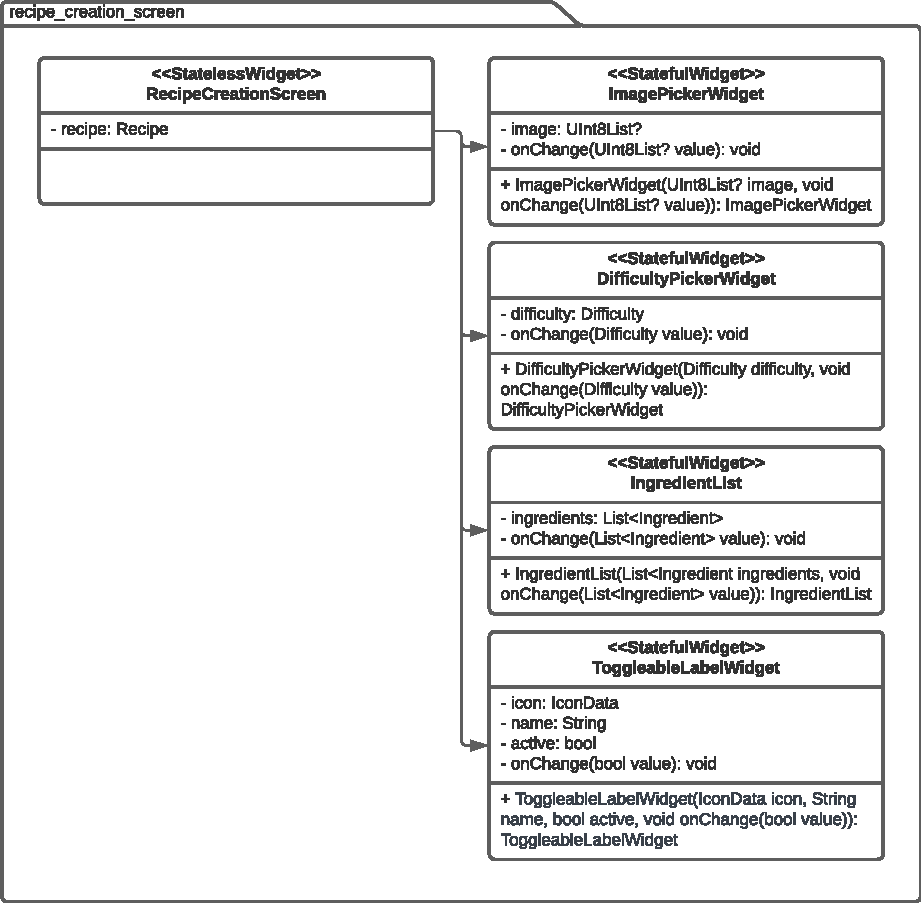
\includegraphics[width=\textwidth]{images/presentationLayer/classDiagrams/recipeCreationScreenWhole.pdf}
    \caption{Klassendiagramm des Pakets recipe\_creation\_screen}
\end{figure}
\newpage
\subsubsection{\texttt{RecipeCreationScreen}}
\label{sec:recipeCreationScreen}
Die Klasse bildet die Rezept-Erstellungs-Ansicht ab. Sie ist ein \texttt{StatelessWidget}, da sie keinen Zustand verwaltet. Dies übernehmen die einzelnen Teilwidgets. Es werden verschiedene Widgets angezeigt, die es ermöglichen Rezeptdaten einzugeben oder abzuändern. Die Klasse verwendet die Klassen \nameref{sec:backButton} und \nameref{sec:portionAmountField} aus dem Package \texttt{ui\_elements}.
\begin{figure}[htp]
    \begin{minipage}
        [t]{0.49\textwidth}
        \centering
        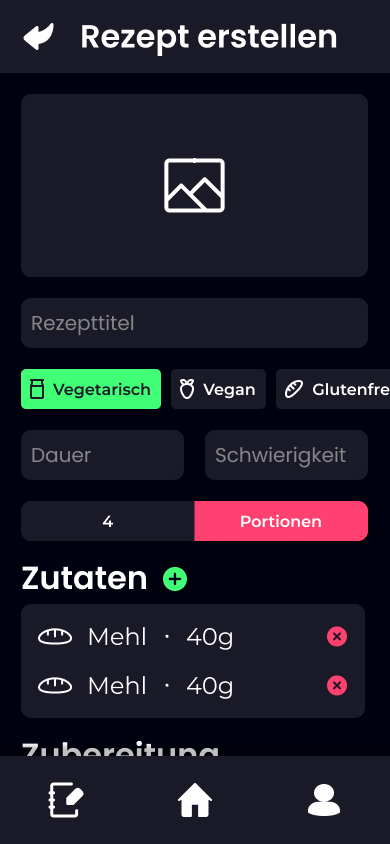
\includegraphics[height=80mm]{images/presentationLayer/uiElements/recipeCreationScreen.jpg}
        \caption{\protect\raggedright Abbildung des Recipe\-Creation\-Screens}
    \end{minipage}
    \begin{minipage}
        [t]{0.49\textwidth}
        \centering
        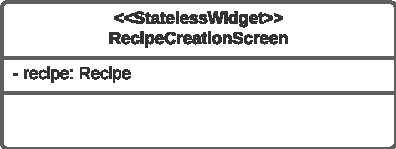
\includegraphics[width=0.95\textwidth]{images/presentationLayer/classDiagrams/recipeCreationScreen.pdf}
        \caption{\protect\raggedright Klassendiagramm des Recipe\-Creation\-Screens}
    \end{minipage}
\end{figure}
\subsubsection*{Attribute}
\paragraph{\texttt{recipe: Recipe}}
Soll ein Rezept verändert werden, so wird das Ursprungsrezept über den \Gls{BuildContext} übergeben und in diesem Parameter gespeichert. Andernfalls bleibt der Wert null.
\subsubsection*{Methoden}
\paragraph{\texttt{createRecipe(): void}}
Leitet über einen Provider die Anfrage zum Erstellen eines Rezepts an den zuständigen Service weiter. Dabei wird das Rezept aus den einzelnen Teilwidgets zusammengesetzt.
\newpage
\subsubsection{\texttt{ImagePickerWidget}}
\label{sec:imagePickerWidget}
Die Klasse stellt ein Widget bereit, mit dem der Nutzer ein Bild auswählen oder löschen kann. Sie ist ein \texttt{StatefulWidget}, da sie den Zustand \texttt{image} verwaltet.
\begin{figure}[htp]
    \begin{minipage}
        [t]{0.49\textwidth}
        \centering
        
\includegraphics[width=.8\textwidth]{images/presentationLayer/uiElements/imagePickerWidget.png}
        \caption{\protect\raggedright Abbildung des Image\-Picker\-Widgets}
    \end{minipage}
    \begin{minipage}
        [t]{0.49\textwidth}
        \centering
        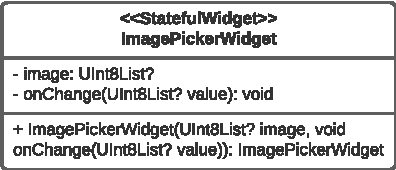
\includegraphics[width=0.95\textwidth]{images/presentationLayer/classDiagrams/imagePickerWidget.pdf}
        \caption{\protect\raggedright Klassendiagramm des Image\-Picker\-Widgets}
    \end{minipage}
\end{figure}
\subsubsection*{Attribute}
\paragraph{\texttt{image: UInt8List?}}
Das ausgewählte Bild. Ist der Wert null, so wurde noch kein Bild ausgewählt.
\paragraph{\texttt{onChange(UInt8List? value): void}}
Callback-Methode, die ausgeführt wird, wenn sich das Bild ändert und das neue Bild als Parameter übergeben bekommt. Ist \texttt{value} null, so soll das Bild gelöscht werden.
\subsubsection*{Methoden}
\paragraph{\texttt{ImagePickerWidget(UInt8List? image, void onChange(UInt8List? value)): ImagePickerWidget}}
Konstruktor, der das Bild und die Callback-Methode übergeben bekommt.
\newpage

\subsubsection{\texttt{DifficultyPickerWidget}}
\label{sec:difficultyPickerWidget}
Die Klasse stellt ein Widget bereit, mit dem der Nutzer die Schwierigkeit des Rezepts auswählen kann. Sie ist ein \texttt{StatefulWidget}, da sie den Zustand \texttt{difficulty} verwaltet. Drückt der Nutzer auf das Widget, öffnet sich ein Drop-Down-Menü, in dem er die Schwierigkeit auswählen kann. 

\begin{figure}[htp]
    \begin{minipage}
        [t]{0.49\textwidth}
        \centering
        
\includegraphics[height=1cm]{images/presentationLayer/uiElements/difficultyPickerWidget.png}
        \caption{\protect\raggedright Abbildung des Difficulty\-Picker\-Widgets}
    \end{minipage}
    \begin{minipage}
        [t]{0.49\textwidth}
        \centering
        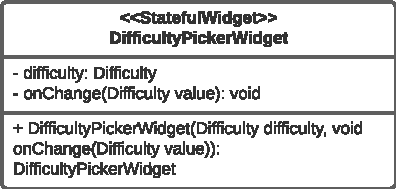
\includegraphics[width=0.95\textwidth]{images/presentationLayer/classDiagrams/difficultyPickerWidget.pdf}
        \caption{\protect\raggedright Klassendiagramm des Difficulty\-Picker\-Widgets}
    \end{minipage}
\end{figure}

\subsubsection*{Attribute}
\paragraph{\texttt{difficulty: Difficulty}}
Die ausgewählte Schwierigkeit.
\paragraph{\texttt{onChange(Difficulty value): void}}
Callback-Methode, die ausgeführt wird, wenn sich die Schwierigkeit ändert und die neue Schwierigkeit als Parameter übergeben bekommt.
\subsubsection*{Methoden}
\paragraph{\texttt{DifficultyPickerWidget(Difficulty difficulty, void onChange(Difficulty value)): DifficultyPickerWidget}}
Konstruktor, der die Schwierigkeit und die Callback-Methode übergeben bekommt.
\newpage
\subsubsection{\texttt{IngredientList}}
\label{sec:ingredientList}
Die Klasse stellt die Liste der Zutaten dar. Sie ist ein \texttt{StatefulWidgget}, da sie den Zustand \texttt{ingredients} verwaltet. Sie erzeugt eine Listenansicht, in der für jedes Rezept ein Item gezeigt wird. Zusätzlich verwendet sie die Klasse \nameref{sec:addButton} und \nameref{sec:removeButton} aus dem Package \texttt{ui\_elements}. Drückt man auf den Knopf, wird man zur Zutaten-Erstellungs-Ansicht (\ref{sec:ingredientCreationScreen}) weitergeleitet.
\begin{figure}[htp]
    \begin{minipage}
        [t]{0.49\textwidth}
        \centering
        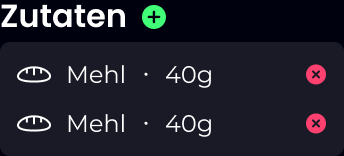
\includegraphics[width=.95\textwidth]{images/presentationLayer/uiElements/ingredientList.png}
        \caption{\protect\raggedright Abbildung der Ingredient\-List}
    \end{minipage}
    \begin{minipage}
        [t]{0.49\textwidth}
        \centering
        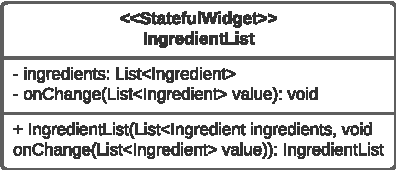
\includegraphics[width=0.95\textwidth]{images/presentationLayer/classDiagrams/ingredientList.pdf}
        \caption{\protect\raggedright Klassendiagramm der Ingredient\-List}
    \end{minipage}
\end{figure}
\subsubsection*{Attribute}
\paragraph{\texttt{ingredients: List<Ingredient>}}
Die Liste der Zutaten.
\paragraph{\texttt{onChange(List<Ingredient> ingredients): void}}
Callback-Methode, die ausgeführt wird, wenn sich die Liste der Zutaten ändert und die neue Liste als Parameter übergeben bekommt.
\subsubsection*{Methoden}
\paragraph{\texttt{IngredientList(List<Ingredient> ingredients, void onChange(List<Ingredient> ingredients)): IngredientList}}
Konstruktor, der die Liste der Zutaten und die Callback-Methode übergeben bekommt.
\newpage
\subsubsection{\texttt{ToggleableLabelWidget}}
\label{sec:toggleableLabelWidget}
Die Klasse repräsentiert ein Label, das aktiviert oder deaktiviert werden kann, indem es gedrückt wird. Es ändert entsprechend seine Farbe. Sie ist ein \texttt{StatefulWidget}, da sie den Zustand \texttt{active} verwaltet. Sie erzeugt ein Text-Widget, das aktiviert oder deaktiviert werden kann, indem es gedrückt wird. Es ändert entsprechend seine Farbe. Es verwendet die Klasse \nameref{sec:tagItem} aus dem Package \texttt{ui\_elements}.
\begin{figure}[htp]
    \begin{minipage}
        [t]{0.49\textwidth}
        \centering
        
\includegraphics[height=1cm]{images/presentationLayer/uiElements/toggleableLabelWidget.png}
        \caption{\protect\raggedright Abbildung des Toggleable\-Label\-Widgets im aktiven Zustand}
    \end{minipage}
    \begin{minipage}
        [t]{0.49\textwidth}
        \centering
        \includegraphics[width=0.95\textwidth]{images/presentationLayer/classDiagrams/toggleableLabelWidget.pdf}
        \caption{\protect\raggedright Klassendiagramm des Toggleable\-Label\-Widgets}
    \end{minipage}
\end{figure}

\subsubsection*{Attribute}
\paragraph{\texttt{icon: IconData}}
Das Icon, das angezeigt wird.
\paragraph{\texttt{name: String}}
Der Name, der angezeigt wird.
\paragraph{\texttt{active: bool}}
Der Zustand, ob das Label aktiviert ist oder nicht.
\paragraph{\texttt{onChange(bool value): void}}
Callback-Methode, die ausgeführt wird, wenn sich der Zustand ändert und den neuen Zustand als Parameter übergeben bekommt.
\subsubsection*{Methoden}
\paragraph{\texttt{ToggleableLabelWidget(IconData icon, String name, bool active, void onChange(bool value)): ToggleableLabelWidget}}
Konstruktor, der das Icon, den Namen, den Zustand und die Callback-Methode übergeben bekommt und setzt.
\newpage

\subsection{\texttt{ingredient\_creation\_screen}}
Das Package \texttt{ingredient\_creation\_screen} enthält alle Klassen für die Zutaten-Erstellungs-Ansicht. Der anzuzeigende Screen ist in der Klasse \hyperref[sec:ingredientCreationScreen]{\texttt{IngredientCreationScreen}} implementiert.
\begin{figure}
    [htp]
    \centering
    \includegraphics[width=0.95\textwidth]{images/presentationLayer/classDiagrams/ingredientCreationScreenWhole.pdf}
    \caption{\protect\raggedright Klassendiagramm des ingredient\_creation\_screen-Packages}
\end{figure}
\newpage
\subsubsection{\texttt{IngredientCreationScreen}}
\label{sec:ingredientCreationScreen}
Die Klasse bildet die Zutaten-Erstellungs-Ansicht ab. Sie ist ein \texttt{StatelessWidget}, da sie selbst keinen Zustand verwaltet. Dies übernehmen die einzelnen Teilwidgets. Es werden verschiedene Widgets angezeigt, die es ermöglichen Zutatendaten einzugeben und Vorschläge für Namen anzuzeigen. Sie verwendet die Klassen \nameref{sec:backButton} aus dem Package \texttt{ui\_elements}.
\begin{figure}[htp]
    \begin{minipage}
        [t]{0.49\textwidth}
        \centering
        \includegraphics[height=8cm]{images/presentationLayer/uiElements/ingredientCreationScreen.jpg}
        \caption{\protect\raggedright Abbildung des Ingredient\-Creation\-Screens}
    \end{minipage}
    \begin{minipage}
        [t]{0.49\textwidth}
        \centering
        \includegraphics[width=0.95\textwidth]{images/presentationLayer/classDiagrams/ingredientCreationScreen.pdf}
        \caption{\protect\raggedright Klassendiagramm des Ingredient\-Creation\-Screens}
    \end{minipage}
\end{figure}
\subsubsection*{Attribute}
\paragraph{\texttt{nameController: TextEditingController}}
Der Controller für den Namen der Zutat.
\paragraph{\texttt{iconName: String}}
Der Name des Icons, das ausgewählt ist.
\paragraph{\texttt{amountController: TextEditingController}}
Der Controller für die Menge der Zutat.
\paragraph{\texttt{unitController: TextEditingController}}
Der Controller für die Einheit der Zutat.
\subsubsection*{Methoden}
\paragraph{\texttt{createIngredient(): void}}
Validiert die Felder und leitet dann zur vorherigen Ansicht zurück, wobei die eingegebenen Daten als \texttt{Ingredient} über den \Gls{BuildContext} übergeben werden.
\newpage
\subsubsection{\texttt{IconPickerWidget}}
\label{sec:iconPickerWidget}
Die Klasse repräsentiert ein Widget, das ein Icon auswählen kann. Es ist ein \texttt{StatefulWidget}, da es den Zustand \texttt{iconName} verwaltet. Drückt der Nutzer auf das Widget öffnet sich ein \Gls{Dialog} mit einer Liste von Icons, aus der der Nutzer eines auswählen kann.
\begin{figure}[htp]
    \begin{minipage}
        [t]{0.49\textwidth}
        \centering
        \includegraphics[height=1cm]{images/presentationLayer/uiElements/iconPickerWidget.png}
        \caption{\protect\raggedright Abbildung des Icon\-Picker\-Widgets}
    \end{minipage}
    \begin{minipage}
        [t]{0.49\textwidth}
        \centering
        \includegraphics[width=0.95\textwidth]{images/presentationLayer/classDiagrams/iconPickerWidget.pdf}
        \caption{\protect\raggedright Klassendiagramm des Icon\-Picker\-Widgets}
    \end{minipage}
\end{figure}
\subsubsection*{Attribute}
\paragraph{\texttt{iconName: String}}
Der Name des Icons, das ausgewählt ist.
\paragraph{\texttt{onChange(String iconName): void}}
Callback-Methode die ausgeführt wird, wenn sich das Icon ändert und den neuen Namen als Parameter übergeben bekommt.
\subsubsection*{Methoden}
\paragraph{\texttt{IconPickerWidget(String iconName, void onChange(String iconName)): IconPickerWidget}}
Konstruktor, der den Namen des Icons und die Callback-Methode übergeben bekommt und setzt.
\newpage
\subsubsection{\texttt{IngredientNameInput}}
\label{sec:ingredientNameInput}
Die Klasse repräsentiert ein Widget, in das ein Name für eine Zutat eingegeben werden kann. Es ist ein \texttt{StatefulWidget}, da es den Zustand \texttt{name} verwaltet. Es werden live Vorschläge angezeigt.
\begin{figure}[htp]
    \begin{minipage}
        [t]{0.49\textwidth}
        \centering
        \includegraphics[height=4cm]{images/presentationLayer/uiElements/ingredientNameInput.png}
        \caption{\protect\raggedright Abbildung des Ingredient\-Name\-Inputs}
    \end{minipage}
    \begin{minipage}
        [t]{0.49\textwidth}
        \centering
        \includegraphics[width=0.95\textwidth]{images/presentationLayer/classDiagrams/ingredientNameInput.pdf}
        \caption{\protect\raggedright Klassendiagramm des Ingredient\-Name\-Inputs}
    \end{minipage}
\end{figure}
\subsubsection*{Attribute}
\paragraph{\texttt{name: String}}
Der Name der Zutat.
\paragraph{\texttt{controller: TextEditingController}}
Der Controller für den Namen der Zutat.
\subsubsection*{Methoden}
\paragraph{\texttt{IngredientNameInput(String name, TextEditingController controller): IngredientNameInput}}
Konstruktor, der den Namen der Zutat und den Controller übergeben bekommt und setzt.
\newpage
\subsection{\texttt{settings\_screen}}
Das Package \texttt{settings\_screen} enthält alle Klassen für die Einstellungsansicht. Der anzuzeigende Screen ist in der Klasse \hyperref[sec:settingsScreen]{\texttt{SettingsScreen}} implementiert.
\begin{figure}
    [htp]
    \centering
    \includegraphics[width=0.95\textwidth]{images/presentationLayer/classDiagrams/settingsScreenWhole.pdf}
    \caption{\protect\raggedright Klassendiagramm des settings\_screen-Packages}
\end{figure}
\newpage

\subsubsection{\texttt{SettingsScreen}}
\label{sec:settingsScreen}
Die Klasse bildet die Einstellungsansicht ab. Sie ist ein \texttt{StatelessWidget}, da sie keinen eigenen Zustand verwaltet.

\begin{figure}[htp]
    \begin{minipage}
        [t]{0.49\textwidth}
        \centering
        \includegraphics[height=8cm]{images/presentationLayer/uiElements/settingsScreen.jpg}
        \caption{\protect\raggedright Abbildung des Settings\-Screens}
    \end{minipage}
    \begin{minipage}
        [t]{0.49\textwidth}
        \centering
        \includegraphics[width=0.95\textwidth]{images/presentationLayer/classDiagrams/settingsScreen.pdf}
        \caption{\protect\raggedright Klassendiagramm des Settings\-Screens}
    \end{minipage}
\end{figure}
\subsubsection*{Methoden}
\paragraph{\texttt{logout(): void}}
Leitet eine Anfrage zum Abmelden des Nutzers über einen Provider an den zuständigen Service weiter. Leitet dann den Nutzer an die Anmeldeseite weiter.
\paragraph{\texttt{deleteAccount(): void}}
Leitet eine Anfrage zum Löschen des Nutzers über einen Provider an den zuständigen Service weiter. Leitet dann den Nutzer an die Anmeldeseite weiter.
\paragraph{\texttt{renameUser(String newName): void}}
Leitet eine Anfrage zum Umbenennen des Nutzers über einen Provider an den zuständigen Service weiter.
\newpage
\subsubsection{\texttt{ProfileImagePicker}}
\label{sec:profileImagePicker}
Die Klasse bildet die Profilbildauswahl ab. Sie ist ein \texttt{StatefulWidget}, da sie den Zustand \texttt{profileImage} verwaltet. Sie zeigt ein Bild an, das der Nutzer auswählen kann.
\begin{figure}[htp]
    \begin{minipage}
        [t]{0.49\textwidth}
        \centering
        \includegraphics[height=3cm]{images/presentationLayer/uiElements/profileImagePicker.png}
        \caption{\protect\raggedright Abbildung des Profile\-Image\-Pickers}
    \end{minipage}
    \begin{minipage}
        [t]{0.49\textwidth}
        \centering
        \includegraphics[width=0.95\textwidth]{images/presentationLayer/classDiagrams/profileImagePicker.pdf}
        \caption{\protect\raggedright Klassendiagramm des Profile\-Image\-Pickers}
    \end{minipage}
\end{figure}
\subsubsection*{Attribute}
\paragraph{\texttt{profileImage: UInt8List?}}
Das Profilbild des Nutzers. Oder \texttt{null}, wenn keines wurde.
\paragraph{\texttt{onChange(UInt8List? profileImage): void}}
Callback-Methode, die ausgeführt wird, wenn sich das Profilbild ändert und das neue Profilbild als Parameter übergeben bekommt.
\subsubsection*{Methoden}
\paragraph{\texttt{ProfileImagePicker(UInt8List? profileImage, void onChange(UInt8List? profileImage)): ProfileImagePicker}}
Konstruktor, der das Profilbild und die Callback-Methode übergeben bekommt und setzt.
\newpage
\subsubsection{\texttt{GroupList}}
\label{sec:groupList}
Die Klasse bildet die Gruppenliste ab. Sie ist ein \texttt{StatelessWidget}, da sie keinen eigenen Zustand verwaltet. Sie zeigt eine Liste von Gruppen an, bei denen der Nutzer Mitglied ist. Die Klasse verwendet die Klassen \nameref{sec:addButton} und \nameref{sec:removeButton} aus dem Package \texttt{ui\_elements}.
\begin{figure}[htp]
    \begin{minipage}
        [t]{0.49\textwidth}
        \centering
        \includegraphics[width=.95\textwidth]{images/presentationLayer/uiElements/groupList.png}
        \caption{\protect\raggedright Abbildung der Group\-List}
    \end{minipage}
    \begin{minipage}
        [t]{0.49\textwidth}
        \centering
        \includegraphics[width=0.95\textwidth]{images/presentationLayer/classDiagrams/groupList.pdf}
        \caption{\protect\raggedright Klassendiagramm der Group\-List}
    \end{minipage}
\end{figure}
\subsubsection*{Attribute}
\paragraph{\texttt{groups: List<Group>}}
Die Liste der Gruppen, die angezeigt werden sollen.
\subsubsection*{Methoden}
\paragraph{\texttt{GroupList(List<Group> groups): GroupList}}
Konstruktor, der die Liste der Gruppen übergeben bekommt und setzt.
\paragraph{\texttt{leaveGroup(String id): void}}
Leitet die Anfrage zum Verlassen der Gruppe über einen Provider an den zuständigen Service weiter.
\newpage
\subsubsection{\texttt{OwnRecipeList}}
\label{sec:ownRecipeList}
Die Klasse bildet die Rezeptliste des Nutzers ab. Sie ist ein \texttt{StatelessWidget}, da sie keinen eigenen Zustand verwaltet. Sie zeigt eine Liste von Rezepten an, die der Nutzer erstellt hat. Sie verwendet die Klassen \nameref{sec:addButton}, \nameref{sec:removeButton} und \nameref{sec:eyeButton} aus dem Package \texttt{ui\_elements}.
\begin{figure}[htp]
    \begin{minipage}
        [t]{0.49\textwidth}
        \centering
        \includegraphics[width=.95\textwidth]{images/presentationLayer/uiElements/ownRecipeList.png}
        \caption{\protect\raggedright Abbildung der OwnRecipeList}
    \end{minipage}
    \begin{minipage}
        [t]{0.49\textwidth}
        \centering
        \includegraphics[width=0.95\textwidth]{images/presentationLayer/classDiagrams/ownRecipeList.pdf}
        \caption{\protect\raggedright Klassendiagramm der OwnRecipe\-List}
    \end{minipage}
\end{figure}
\subsubsection*{Attribute}
\paragraph{\texttt{recipes: List<Recipe>}}
Die Rezepte, die angezeigt werden sollen.
\subsubsection*{Methoden}
\paragraph{\texttt{OwnRecipeList(List<Recipe> recipes): OwnRecipeList}}
Konstruktor, der die Rezepte übergeben bekommt und setzt.
\paragraph{\texttt{hideRecipe(String id): void}}
Leitet eine Anfrage zum Setzen des Rezepts auf privat über einen Provider an den zuständigen Service weiter.
\paragraph{\texttt{exportRecipe(Recipe recipe): void}}
Leitet eine Anfrage zum Exportieren des Rezepts über einen Provider an den zuständigen Service weiter.
\paragraph{\texttt{deleteRecipe(String id): void}}
Leitet eine Anfrage zum Löschen des Rezepts über einen Provider an den zuständigen Service weiter.
\newpage
\subsection{\texttt{group\_detail\_screen}}
Das Package \texttt{group\_detail\_screen} enthält alle Klassen für die Gruppen-Detaill-Ansicht. Der anzuzeigende Screen ist in der Klasse \hyperref[sec:groupDetailScreen]{\texttt{GroupDetailScreen}} implementiert.
\begin{figure}
    [htp]
    \centering
    \includegraphics[width=0.95\textwidth]{images/presentationLayer/classDiagrams/groupDetailScreenWhole.pdf}
    \caption{\protect\raggedright Klassendiagramm des group\_detail\_screen-Packages}
\end{figure}
\newpage
\subsubsection{\texttt{GroupDetailScreen}}
\label{sec:groupDetailScreen}
Die Klasse bildet die Gruppen-Detail-Ansicht ab. Sie ist ein \texttt{StatefulWidget}, da sie den Zustand \texttt{group} verwaltet. Sie verwendet die Klasse \nameref{sec:backButton} aus dem Package \texttt{ui\_elements}.
\begin{figure}[htp]
    \begin{minipage}
        [t]{0.49\textwidth}
        \centering
        \includegraphics[height=8cm]{images/presentationLayer/uiElements/groupDetailScreen.jpg}
        \caption{\protect\raggedright Abbildung der Gruppen-Detail-Ansicht}
    \end{minipage}
    \begin{minipage}
        [t]{0.49\textwidth}
        \centering
        \includegraphics[width=0.95\textwidth]{images/presentationLayer/classDiagrams/groupDetailScreen.pdf}
        \caption{\protect\raggedright Klassendiagramm des GroupDetailScreens}
    \end{minipage}
\end{figure}
\subsubsection*{Attribute}
\paragraph{\texttt{group: Group}}
Die Gruppe, deren Details angezeigt werden sollen. Wird bei der Initialisierung aus dem \Gls{BuildContext} gelesen.
\subsubsection*{Methoden}
\paragraph{\texttt{deleteGroup(): void}}
Leitet eine Anfrage über einen Provider an den zugehörigen Service weiter, um die Gruppe aufzulösen.
\paragraph{\texttt{renameGroup(String newName): void}}
Leitet eine Anfrage über einen Provider an den zugehörigen Service weiter, um die Gruppe umzubenennen.
\paragraph{\texttt{leaveGroup(): void}}
Leitet eine Anfrage über einen Provider an den zugehörigen Service weiter, um die Gruppe zu verlassen.
\paragraph{\texttt{shareGroupCode(): void}}
Kopiert das Gruppenkürzel in die Zwichenablage zum Teilen.
\newpage
\subsubsection{\texttt{MemberList}}
\label{sec:memberList}
Die Klasse stellt ein Widget bereit, das die eine Liste der Gruppenmitglieder zeigt. Sie verwendet die Klasse \nameref{sec:addButton} aus dem Package \texttt{ui\_elements}.
\begin{figure}[htp]
    \begin{minipage}
        [t]{0.49\textwidth}
        \centering
        \includegraphics[height=5cm]{images/presentationLayer/uiElements/memberList.png}
        \caption{\protect\raggedright Abbildung der MemberList}
    \end{minipage}
    \begin{minipage}
        [t]{0.49\textwidth}
        \centering
        \includegraphics[width=0.95\textwidth]{images/presentationLayer/classDiagrams/memberList.pdf}
        \caption{\protect\raggedright Klassendiagramm des MemberList}
    \end{minipage}
\end{figure}
\subsubsection*{Attribute}
\paragraph{\texttt{members: List<GroupMember>}}
Die Mitglieder der Gruppe.
\subsubsection*{Methoden}
\paragraph{\texttt{MemberList(List<GroupMember> members): MemberList}}
Konstruktor, der die Miglieder der Gruppe entgegen nimmt und setzt.
\paragraph{\texttt{makeAdmin(String userId): void}}
Leitet eine Anfrage zum Ernennen zum Administrator über einen Provider an den zugehörigen Service weiter.
\paragraph{\texttt{removeAdminStatus(String userId): void}}
Leitet eine Anfrage zum Entfernen des Administratorstatus über einen Provider an den zugehörigen Service weiter.
\paragraph{\texttt{kickUser(String userId): void}}
Leitet eine Anfrage zum Kicken eines Nutzers über einen Provider an den zugehörigen Service weiter.
\paragraph{\texttt{banUser(String userId): void}}
Leitet eine Anfrage zum Bannen eines Nutzers über einen Provider an den zugehörigen Service weiter.
\newpage
\subsubsection{\texttt{GroupRecipeList}}
\label{sec:groupRecipeList}
Die Klasse stellt ein Widget bereit, das die eine Liste der Rezepte in einer Gruppe zeigt. Sie verwendet die Klasse \nameref{sec:eyeButton} aus dem Package \texttt{ui\_elements}.
\begin{figure}[htp]
    \begin{minipage}
        [t]{0.49\textwidth}
        \centering
        \includegraphics[height=5cm]{images/presentationLayer/uiElements/groupRecipeList.png}
        \caption{\protect\raggedright Abbildung der GroupRecipeList}
    \end{minipage}
    \begin{minipage}
        [t]{0.49\textwidth}
        \centering
        \includegraphics[width=0.95\textwidth]{images/presentationLayer/classDiagrams/groupRecipeList.pdf}
        \caption{\protect\raggedright Klassendiagramm des GroupRecipeList}
    \end{minipage}
\end{figure}
\subsubsection*{Attribute}
\paragraph{\texttt{recipes: List<GroupRecipe>}}
Die Rezepte der Gruppe.
\subsubsection*{Methoden}
\paragraph{\texttt{GroupRecipeList(List<GroupRecipe> recipes): MemberList}}
Konstruktor, der die Rezepte der Gruppe entgegen nimmt und setzt.
\paragraph{\texttt{toggleCensoring(String recipeId): void}}
Leitet eine Anfrage zum Aktivieren/Deaktivieren des \glslink{ausblenden}{Ausblenden} eines Rezepts über einen Provider an den zugehörigen Service weiter.
\newpage
\subsection{\texttt{QRCodeScreen}}
\label{sec:qrCodeScreen}
Die Klasse bildet die QR-Code-Ansicht ab. Sie ist ein \texttt{StatelessWidget}, da sie selbst keinen Zustand verwaltet. Sie zeigt einen QR-Code an, der den Nutzer zu einer Gruppe hinzufügt, wenn er gescannt wird.
\begin{figure}[htp]
    \begin{minipage}
        [t]{0.49\textwidth}
        \centering
        \includegraphics[height=8cm]{images/presentationLayer/uiElements/qrCodeScreen.jpg}
        \caption{\protect\raggedright Abbildung des QR\-Code\-Screens}
    \end{minipage}
    \begin{minipage}
        [t]{0.49\textwidth}
        \centering
        \includegraphics[width=0.95\textwidth]{images/presentationLayer/classDiagrams/qrCodeScreen.pdf}
        \caption{\protect\raggedright Klassendiagramm des QR\-Code\-Screens}
    \end{minipage}
\end{figure}
\subsubsection*{Attribute}
\paragraph{\texttt{group: Group}}
Die Gruppe, die der QR-Code repräsentiert. Sie wird bei der Initialisierung aus dem \Gls{BuildContext} gelesen.

\newpage
\section{REST-Webservice}
Um seinen Account zu verwalten, Rezepte aufzurufen oder mit Gruppen interagieren zu können, benötigt man die Verbindung zum Server.
Um die Anfragen performant und flexibel zu gestalten, verwendet das Projekt \glslink{nodejs}{Node.js} in Verbindung mit dem \glslink{expressjs}{Express.js} Framework.
\glslink{expressjs}{Express.js} ermöglicht es, einfach einen robusten Webservice zu entwickeln. Dazu bietet Express.js eine Menge an Dienstprogrammmethoden an.
Als Programmiersprache verwenden wir Serverseitig \glslink{typescript}{TypeScript}. \glslink{typescript}{TypeScript} ist eine freie und quelloffene Programmiersprache, die statische Typisierung zu \glslink{javascript}{JavaScript} hinzufügt.
Dies ermöglicht die Verwendung von Sprachkonstrukten wie Klassen, Vererbungen und Modulen, um unser Projekt sowohl client- als auch serverseitig objektorientiert zu entwickeln.
Dies vereinfacht die Strukturierung des Serveraufbaus und garantiert die Langzeitwartbarkeit. Mit TypeScript als eine der meistgenutzten Programmiersprachen und Node.js als eine der beliebtesten Technologien wollen wir zudem eine hohe Zukunftssicherheit mit unserer Wahl garantieren.

Anfragen an den Server erfolgen über eine HTTP-Anfrage, an eine bestimmte URL. Diese URL besteht zum einen aus der IP-Adresse des Servers und zum anderen aus einem Pfad, der die gewünschte Aktion beschreibt. Mehr dazu im Kapitel \ref{sec:HTTP-Anfragen und API-Endpunkte}.
Die Anfragen erfolgen dabei an eine \glslink{rest}{REST-API} (Representational State Transfer Application Programming Interface). REST ist ein Programmierparadigma für verteilte Systeme, insbesondere für Webservices.
Die \glslink{rest}{REST-API} ist dabei eine Schnittstelle, die es ermöglicht, dass ein Client mit dem Server kommunizieren kann.
Die Anfrage enthält dabei Informationen über die gewünschte Aktion und die Daten, die für die Ausführung der Aktion benötigt werden.
Der Server verarbeitet die Anfrage und sendet eine Antwort zurück.
Die Antwort enthält dabei Informationen über den Erfolg der Anfrage und die Daten, die für die Ausführung der Aktion benötigt werden.

Ein vollständiges Klassendiagramm des Backends befindet sich im Anhang (\autoref{fig:classDiagramBackend}).

\newpage

\subsection{\texttt{Server}}\label{sec:Server}
In einer Express-Anwendung bezieht sich der Begriff "Server" auf die Hauptkomponente, die die Anfragen von Clients empfängt.
Der Server ist dafür verantwortlich, die Verbindung mit der Datenbank und Firebase (Kapitel \ref{sec:Nutzerverwaltung}) aufzubauen und die Server-Applikation zu starten.

\begin{figure}[htp]
    \centering
    \includegraphics[width = 0.3\textwidth]{images/webserver/server.pdf}
    \caption{Klasse Server des Webservers}
    \label{fig:server}
\end{figure}

\subsection*{Attribute}
\paragraph{\texttt{port: number}}
Durch das Attribut \texttt{port} wird bestimmt, auf welchem Port Anfragen an den Server zulässig sind. Es soll möglich sein, die Wahl des Ports durch eine Umgebungsvariable zu wählen. Wird kein Port durch eine Umgebungsvariable definiert, so soll der Server über den Port 3000 erreichbar sein. Es handelt sich um ein privates Attribut.
\texttt{Port} ist vom Type number.
\paragraph{\texttt{express: express.Application}}
Express repräsentiert die Express-Applikation, die beim Start durch \texttt{express.listen()} Anfragen an den Port annimmt.
Express ist vom Typ express.Application. Es handelt sich um ein privates Attribut.
\paragraph{\texttt{application: Application}}
Application vom Typ Application repräsentiert das nach dem Start erzeugte Objekt der Klasse Application. Es handelt sich um ein privates Attribut.
\paragraph{\texttt{database: Database}}
Das Attribut für die Datenbank. Es repräsentiert das nach dem Start erzeugte Objekt der Klasse Database. \texttt{database} ist vom Typ \texttt{Database}. Es handelt sich um ein privates Attribut.

\subsection*{Methoden}
\paragraph{\texttt{Server(): void}}
Konstruktor der Klasse Server, die beim Starten des Servers aufgerufen wird um ein neues Objekt der Klasse Server zu erzeugen. Der Konstruktor gibt keinen Wert zurück.
\paragraph{\texttt{start(): void}}
Durch Aufruf der Funktion \texttt{start()} wird der Server gestartet. Dazu werden in der Funktion die privaten Funktionen \texttt{connectToDatabase()}, \texttt{connectToFirebase()} und \texttt{createServer()} aufgerufen. Die Funktion gibt keinen Wert zurück.
Es handelt sich um eine öffentliche Funktion.
\paragraph{\texttt{connectToDatabase(): boolean}}
Diese Funktion wird benötigt, um die Verbindung der Datenbank herzustellen. Bei erfolgreicher Verbindung wird \texttt{true} zurückgegeben. Beim Fehlerfall wird \texttt{false} zurückgegeben. Es handelt sich um eine private Funktion.
\paragraph{\texttt{connectToFirebase(): boolean}}
Durch diese Funktion wird die Verbindung mit Firebase aufgebaut. Bei erfolgreicher Verbindung wird \texttt{true} zurückgegeben. Beim Fehlerfall wird \texttt{false} zurückgegeben. Es handelt sich um eine private Funktion.
\paragraph{\texttt{createServer(): boolean}}
Beim Aufrufen der \texttt{createServer}-Funktion wird der Server mithilfe von \texttt{express.listen()} gestartet. Beim erfolgreichen Starten des Servers wird \texttt{true} zurückgegeben. Beim Fehlerfall wird \texttt{false} zurückgegeben. Es handelt sich um eine private Funktion.

\newpage

\subsection{\texttt{Application}}\label{sec:Application}
Die \texttt{Application}-Klasse wird durch den Aufruf von \texttt{express()} erstellt, der eine neue Express-Anwendung erzeugt. Dieses \texttt{express()}-Objekt enthält eine Reihe von Methoden, die verwendet werden können, um \nameref{sec:Router}, \nameref{sec:Middleware} und andere Funktionen zu definieren, die für den Betrieb der Anwendung erforderlich sind.

\begin{figure}[htp]
    \centering
    \includegraphics[width = 0.3\textwidth]{images/webserver/application.pdf}
    \caption{Klasse Application des Webservers}
    \label{fig:application}
\end{figure}


\subsubsection*{Attribute}
\paragraph{\texttt{application: express.Application}}
Das Attribut \texttt{application} speichert die \newline
\texttt{express.Application}, die beim erzeugen des Objekts dem Konstruktor übergeben wird.
Durch dieses Attribut bekommt die Klasse Application mitgeteilt, auf welcher \texttt{express.Application} die in dieser Klasse erzeugten Routing-Punkte angewendet werden sollen.
\texttt{Application} ist vom Typ \texttt{express.Application}.
\paragraph{\texttt{authentificationRoutes: AuthenticationRouter}}
Dieses Attribut repräsentiert den \newline
\texttt{AuthenticationRouter}. \texttt{AuthenthificationRouter} ist vom Typ \texttt{AuthenticationRouter}.
\paragraph{\texttt{recipeRoutes: RecipeRouter}}
Dieses Attribut repräsentiert den \texttt{RecipeRouter}. \texttt{RecipeRouter} ist vom Typ \texttt{RecipeRouter}.
\paragraph{\texttt{groupRoutes: GroupRouter}}
Dieses Attribut repräsentiert den \texttt{GroupRouter}. \texttt{GroupRouter} ist vom Typ \texttt{GroupRouter}.
\paragraph{\texttt{userRoutes: UserRouter}}
Dieses Attribut repräsentiert den \texttt{UserRouter}. \texttt{UserRouter} ist vom Typ \texttt{UserRouter}.
\paragraph{\texttt{adminRouter: AdminRouter}}
Dieses Attribut repräsentiert den \texttt{AdminRouter}. \texttt{AdminRouter} ist vom Typ \texttt{AdminRouter}.
\paragraph{\texttt{ingredientRouter: IngredientRouter}}
Dieses Attribut repräsentiert den \texttt{IngredientRouter}. \texttt{IngredientRouter} ist vom Typ \texttt{IngredientRouter}.

\subsubsection*{Methoden}
\paragraph{\texttt{initializeMiddleware(): void}}
Mit dieser Methode wird die \nameref{sec:Middleware} initialisiert. Hier ist es möglich, die eingehenden Anfragen vorzubehandeln, bevor sie an die eigentlichen Routestellen weitergeleitet werden.
Eine Middleware, die zum Beispiel zwischengeschaltet werden kann, wäre \glslink{morgan}{Morgan}. \glslink{morgan}{Morgan} ermöglicht es, \glslink{http-anfragen}{HTTP-Anfragen} zu loggen.
\paragraph{\texttt{initializeRoutes(): void}}
Mit dieser Methode werden die Routen initialisiert.
Es werden jeweilige Routes für jeden Router initialisiert. Diese werden benötigt, um die Anfragen an die richtigen Stellen weiterzuleiten.
Wie genau diese Routen definiert sind wird im Abschnitt \nameref{sec:HTTP-Anfragen und API-Endpunkte} erklärt.
\paragraph{\texttt{initializeErrorHandler(): void}}
Mit dieser Methode wird der Error-Handler initialisiert. Dieser wird benötigt, wenn beispielsweise eine Anfrage an keine gültige Route gestellt wird.

\newpage

\subsection{\texttt{Database}}\label{sec:Database}
Die Datenbank-Klasse ist dafür verantwortlich, die Verbindung mit der Datenbank herzustellen und die Datenbank zu initialisieren.
Zudem wird über diese Klasse der Zugriff auf die Datenbank ermöglicht.
Dafür wird ein Pool von Verbindungen zur Datenbank erstellt.
Eine Pool-Verbindung zu einer Datenbank ist eine Technik, die verwendet wird, um die Effizienz und Skalierbarkeit von Datenbankverbindungen in Anwendungen zu verbessern.
Statt für jede Anfrage eine neue Verbindung zur Datenbank aufzubauen und anschließend wieder zu schließen, werden vorab eine Gruppe von Verbindungen (Pool) erstellt und beibehalten.
Auf diese Klasse wird das \glslink{Singleton}{Singleton-Pattern} angewendet, um sicherzustellen, dass nur eine Instanz der Klasse erzeugt wird.
Die Klasse verwendet das Paket \texttt{pg} um die Verbindung zur Datenbank herzustellen.

\begin{figure}[htp]
    \centering
    \includegraphics[width = 0.3\textwidth]{images/webserver/database.pdf}
    \caption{Klasse Database des Webservers}
    \label{fig:database}
\end{figure}

\subsection*{Attribute}
\paragraph{\texttt{instance: Database}}
Das Attribut \texttt{instance} speichert die Instanz der Klasse \texttt{Database}, die beim erzeugen des Objekts dem Konstruktor mitgeben wird.
Dieses wird benötigt um sicherzustellen, dass nur eine Instanz der Klasse erzeugt wird.
\paragraph{\texttt{pool: pg.Pool}}
Das Attribut \texttt{pool} speichert den Pool von Verbindungen zur Datenbank.
\subsection*{Methoden}
\paragraph{\texttt{Database(): void}}
Konstruktor der Klasse Database, die beim Starten des Servers aufgerufen wird, um ein neues Objekt der Klasse Database zu erzeugen. Der Konstruktor gibt keinen Wert zurück.
Wird der Konstruktor ein weiteres mal aufgerufen, so wird die bereits erzeugte Instanz der Klasse zurückgegeben.
\paragraph{\texttt{cratePool(): void}}
Mit dieser Methode wird der Pool von Verbindungen zur Datenbank erstellt.
\paragraph{\texttt{getPool(): pg.Pool}}
Mit dieser Methode wird der Pool von Verbindungen zur Datenbank zurückgegeben.


\subsection{Router} \label{sec:Router}
Ein Router kann als eine Art Zwischenschicht betrachtet werden, die \glslink{http-anfragen}{HTTP-Anfragen} an die entsprechenden \nameref{sec:Controller} weiterleitet.
Er hilft dabei, den Code zu strukturieren und die Handhabung von Routen in einer modularen und organisierten Weise zu ermöglichen.
Ein Router in Express wird durch die Verwendung des \texttt{express.Router}-Objekts erstellt.
Dieses Objekt stellt eine Miniaturversion der Express-Anwendung dar und kann Routen und Endpunkte definieren, ähnlich wie die Hauptanwendung.
Ein Router kann mit einem Pfad oder Präfix konfiguriert werden, der angibt, unter welchem Pfad seine Routen verfügbar sein sollen.

Ein Router kann dabei mehrere Routen definieren, indem verschiedene HTTP-Methoden wie \texttt{GET}, \texttt{POST}, \texttt{DELETE} usw. verwendet werden.
Jede Route kann einen oder mehrere Handler haben, die ausgeführt werden, wenn die Route mit einer Anfrage übereinstimmt.
Diese Handler sind Funktionen, die Zugriff auf die Anfrage- und Antwortobjekte haben und die erforderlichen Aktionen durchführen.
Router ermöglichen es, den Code in einer Express-Anwendung besser zu organisieren, indem sie verwandte Routen und deren Handler gruppieren.
Dies erleichtert die Wartung, Skalierbarkeit und Lesbarkeit des Codes.

\begin{figure}[htp]
    \centering
    \includegraphics[width = 1\textwidth]{images/webserver/router.pdf}
    \caption{Router-Klassen des Webservers}
    \label{fig:router}
\end{figure}

\subsubsection{\texttt{AbstractRouter}}\label{sec:AbstractRouter}
Der \texttt{AbstractRouter} ist eine abstrakte Repräsentation eines Routers. So kann ein grundlegender Aufbau für alle Router garantiert werden. Alle Router erben von dieser Klasse \texttt{AbstractRouter}.
\subsubsection*{Attribute}
\paragraph{\texttt{router: express.Router}}
Attribut, dass einen Router in Express repräsentiert. Das zugehörige Objekt soll beim Konstruktoraufruf erzeugt werden.
\paragraph{\texttt{controller: AbstractController}}
Attribut, das einen abstrakten Controller repräsentiert. Mit diesem Attribut wird in den jeweiligen Routern der dazu passende Controller gespeichert.
\paragraph{\texttt{checkAuthorization: CheckAuthorization}}
Attribut, das eine Instanz der Klasse \texttt{Check\-Authorization} repräsentiert. Diese Klasse wird benötigt, um die Anfragen an die Routen zu überprüfen.
\paragraph{\texttt{authChecker: express.RequestHandler}}
Attribut, das eine Funktion repräsentiert, die die Anfragen an die Routen überprüft. Diese Funktion wird benötigt, um die Anfragen an die Routen zu überprüfen.

\subsubsection*{Methoden}
\paragraph{\texttt{AbstractRouter(): void}}
Die Methode ist der Konstruktor der Klasse \texttt{AbstractRouter}.
\paragraph{\texttt{abstract setupRoutes(): void}}
Diese abstrakte Methode definiert einen Methode, die die \glslink{childclass}{Kindklassen} implementieren müssen.
\paragraph{\texttt{getRouter(): express.Router}}
Getter-Methode für das Attribut \texttt{router}.

\subsubsection{\texttt{AuthenticationRouter}}\label{sec:AuthenticationRouter}
Der \texttt{AuthenticationRouter} ist speziell für die Verarbeitung von Authentifizierungsanfragen zuständig.
\subsubsection*{Methoden}
\paragraph{\texttt{AuthenthificationRouter():void}}
Die Methode ist der Konstruktor der Klasse \texttt{AuthenticationRouter\\}.
\paragraph{\texttt{setupRoutes(): void}}
Mit dieser Methode werden die Handler im jeweiligen Controller den zugehörigen Routestellen zugewiesen.

\subsubsection{\texttt{RecipeRouter}}\label{sec:RecipeRouter}
Der \texttt{RecipeRouter} ist für die Verwaltung der Routen und Endpunkte verantwortlich, die mit Rezepten zusammenhängen.
\subsubsection*{Methode}
\paragraph{\texttt{RecipeRouter():void}}
Die Methode ist der Konstruktor der Klasse \texttt{RecipeRouter}.
\paragraph{\texttt{setupRoutes(): void}}
Mit dieser Methode werden die Handler im jeweiligen Controller den zugehörigen Routestellen zugewiesen.

\subsubsection{\texttt{GroupRouter}}\label{sec:GroupRouter}
Der \texttt{GroupRouter} ist verantwortlich für die Verwaltung der Routen und Endpunkte, die mit Gruppen in der Anwendung zusammenhängen.
\subsubsection*{Methode}
\paragraph{\texttt{GroupRouter():void}}
Die Methode ist der Konstruktor der Klasse \texttt{GroupRouter}.
\paragraph{\texttt{setupRoutes(): void}}
Mit dieser Methode werden die Handler im jeweiligen Controller den zugehörigen Routestellen zugewiesen.

\subsubsection{\texttt{UserRouter}}\label{sec:UserRouter}
Der \texttt{UserRouter} ist für die Verwaltung von Routen und Endpunkten zuständig, die mit Benutzeraktionen und -informationen zusammenhängen.
\subsubsection*{Methode}
\paragraph{\texttt{UserRouter():void}}
Die Methode ist der Konstruktor der Klasse \texttt{UserRouter}.
\paragraph{\texttt{setupRoutes(): void}}
Mit dieser Methode werden die Handler im jeweiligen Controller den zugehörigen Routestellen zugewiesen.

\subsubsection{\texttt{IngredientRouter}}\label{sec:IngredientRouter}
Der \texttt{IngredientRouter} ist verantwortlich für die Verwaltung von Routen und Endpunkten, die mit Zutaten in der Anwendung zusammenhängen.
\subsubsection*{Methode}
\paragraph{\texttt{IngredientRouter():void}}
Die Methode ist der Konstruktor der Klasse \texttt{IngredientRouter}.
\paragraph{\texttt{setupRoutes(): void}}
Mit dieser Methode werden die Handler im jeweiligen Controller den zugehörigen Routestellen zugewiesen.

\subsubsection{\texttt{AdminUserRouter}}\label{sec:AdminUserRouter}
Der \texttt{AdminUserRouter} ist verantwortlich für die Verwaltung von Routen und Endpunkten, die mit Administratorinteraktionen zusammenhängen.
\subsubsection*{Methoden}
\paragraph{\texttt{AdminUserRouter():void}}
Die Methode ist der Konstruktor der Klasse \texttt{AdminUserRouter}.
\paragraph{\texttt{setupRoutes(): void}}
Mit dieser Methode werden die Handler im jeweiligen Controller den zugehörigen Routestellen zugewiesen.

\newpage

\subsection{Middleware} \label{sec:Middleware}
Durch die Middleware können Anfragen vorher bearbeitet werden, bevor sie zu den eigentlichen Controllern gehen.
So kann beispielsweise geprüft werden ob ein Nutzer den Adminstatus in einer Gruppe hat bevor er eine Anfrage an einen Controller stellen darf.
Es wird in der Middelware zudem geprüft, ob der Nutzer überhaupt eine gültige Anfrage stellen darf.

\begin{figure}[htp]
    \centering
    \includegraphics[width = 1\textwidth]{images/webserver/middleware.pdf}
    \caption{Middleware-Klassen des Webservers}
    \label{fig:middleware}
\end{figure}

\subsubsection{\texttt{CheckAuthorization}}\label{sec:CheckAuthorization}
Mit \texttt{CheckAuthorization} kann vor einer Anfrage an einen Router überprüft werden, ob die Anfrage des Nutzers mit validem Firebase \glslink{id-token}{ID-Token} kommt (Kapitel \ref{sec:HTTP-Anfragen und API-Endpunkte}).
\subsubsection*{Methoden}
\paragraph{\texttt{CheckAuthorization(): void)}}
Die Methode ist der Konstruktor der Klasse \texttt{CheckAuthoriza\-tion}.
\paragraph{\texttt{authChecker(req: express.Request, res: express.Response, next: express.NextFunc\-tion): Promise<void>}}
Mit dieser Methode wird durch eine Abfrage an Firebase überprüft, ob das \glslink{id-token}{ID-Token} valide ist. Die Methode ist asynchron und gibt ein \texttt{Promise}-Objekt zurück.

\subsubsection{\texttt{CheckAdminStatus}}\label{sec:CheckAdminStatus}
Mit \texttt{CheckAdminStatus} kann vor einer Anfrage an einen Router überprüft werden, ob der Nutzer den Adminstatus in einer Gruppe hat.
\subsubsection*{Methoden}
\paragraph{\texttt{CheckAdminStatus(): void)}}
Die Methode ist der Konstruktor der Klasse \texttt{CheckAdminStatus}.
\paragraph{\texttt{adminStatusChecker(req: express.Request, res: express.Response, next: express.\-NextFunction): Promise<void>}}
Mit dieser Methode wird überprüft, ob der Nutzer den Adminstatus in einer Gruppe hat. Es wird in der Datenbank geprüft, ob der Nutzer den Adminstatus in der jeweiligen Gruppe hat. Die Methode ist asynchron und gibt ein \texttt{Promise}-Objekt zurück.

\newpage

\subsection{Controller}\label{sec:Controller}
In einer Express-Anwendung bezieht sich der Begriff "Controller" auf eine Komponente oder eine Sammlung von Funktionen, die dazu dienen, die Logik für bestimmte Routen oder Endpunkte zu implementieren.
Der Controller ist für die Verarbeitung von Anfragen, die an eine bestimmte Route gesendet werden und für die Rückgabe von entsprechenden Antworten zuständig.
Ein Controller ist ein Objekt, das Handler-Funktionen für verschiedene Routen bereitstellt.
Diese Handler-Funktionen werden als Callback-Funktionen für die entsprechenden Routen registriert und nehmen die Anfrage (\texttt{req}) und die Antwort (\texttt{res}) als Parameter entgegen.


\begin{figure}[htp]
    \centering
    \includegraphics[width = 1\textwidth]{images/webserver/controller.pdf}
    \caption{Controller Klassen des Webservers}
    \label{fig:controller}
\end{figure}

\subsubsection{\texttt{AbstractController}}\label{sec:AbstractController}
Der \texttt{AbstractController} beschreibt eine abstrakte Darstellung eines Controllers. Alle Controller erben von dieser Klasse.
\subsection*{Attribute}
\paragraph{\texttt{database: Database}}
Attribut, das eine Instanz der Klasse \texttt{Database} repräsentiert. Diese Klasse wird benötigt, um auf die Datenbank zugreifen zu können.
\paragraph{\texttt{pool: pg.Pool}}
Attribut, dass eine Poolverbindung zur Datenbank repräsentiert. Diese Klasse wird benötigt, um auf die Datenbank zugreifen zu können.
\subsection*{Methode}
\paragraph{\texttt{AbstractController(): void}}
Die Methode ist der Konstruktor der Klasse \texttt{AbstractControl\-ler}.

\subsubsection{\texttt{AuthentificationController}}\label{sec:AuthentificationController}
Der \texttt{AuthentificationController} ist verantwortlich für alle Anfragen, die mit der Nutzerverwaltung in Firebase (Kapitel \ref{sec:Nutzerverwaltung}) direkt etwas zu zun haben. Das heißt konkret das Registrieren, Einloggen und Zurücksetzen des Passwort des Nutzers.
\subsubsection*{Methoden}
\paragraph{\texttt{AuthentificationController(): Promise<void>\\}}
Die Methode ist der Konstruktor der Klasse \texttt{AuthentificationController}.
\paragraph{\texttt{public userRegister(req: express.Request, res: express.Response): Promise<void>\\}}
Diese Methode sorgt dafür, dass der Nutzer sich registrieren kann. Der \texttt{req}-Parameter enthält Informationen über den eingehenden HTTP-Request, der Daten wie Benutzername, Passwort und andere Informationen übermittelt. Der \texttt{res}-Parameter wird verwendet, um eine Antwort auf den Request zu senden, beispielsweise um dem Benutzer mitzuteilen, ob die Registrierung erfolgreich war oder Fehler aufgetreten sind.
Die Methode ist asynchron und gibt ein \texttt{Promise}-Objekt zurück.
\paragraph{\texttt{public userLogin(req: express.Request, res: express.Response): Promise<void>\\}}
Diese Methode sorgt dafür, dass der Nutzer sich einloggen kann. Der \texttt{req}-Parameter enthält Informationen über den eingehenden HTTP-Request, der Daten wie Benutzername, Passwort und andere Informationen übermittelt. Der \texttt{res}-Parameter wird verwendet, um eine Antwort auf den Request zu senden, beispielsweise um dem Benutzer mitzuteilen, ob das Einloggen erfolgreich war oder Fehler aufgetreten sind.
Die Methode ist asynchron und gibt ein \texttt{Promise}-Objekt zurück. 
\paragraph{\texttt{userResetPassword(req: express.Request, res: express.Response): Promise<void>\\}}
Diese Methode sorgt dafür, dass der Nutzer sein Passwort zurücksetzen lassen kann. Der \texttt{req}-Parameter enthält Informationen über den eingehenden HTTP-Request, der Daten wie Benutzername übermittelt. Der \texttt{res}-Parameter wird verwendet, um eine Antwort auf den Request zu senden, beispielsweise um dem Benutzer mitzuteilen, ob die Anfrage zum Zurücksetzen des Passworts erfolgreich war oder Fehler aufgetreten sind. Die Methode ist asynchron und gibt ein \texttt{Promise}-Objekt zurück.
\paragraph{\texttt{userGetByToken(req: express.Request, res: express.Response): Promise<void>
\\}}
Diese Methode sorgt dafür, dass der Nutzer anhand seines Tokens abgerufen werden kann. Der \texttt{req}-Parameter enthält Informationen über den eingehenden HTTP-Request, der Daten wie Token übermittelt. Der \texttt{res}-Parameter wird verwendet, um eine Antwort auf den Request zu senden, beispielsweise um dem Nutzer mitzuteilen, ob das Abrufen des Nutzers erfolgreich war oder Fehler aufgetreten sind. Die Methode ist asynchron und gibt ein \texttt{Promise}-Objekt zurück.
\paragraph{\texttt{userRefreshToken(req: express.Request, res: express.Response): Promise<void>\\}}
Diese Methode sorgt dafür, dass der Nutzer sein \texttt{\glslink{id-token}{ID-Token}} aktualisieren kann. Der \texttt{req}-Parameter enthält Informationen über den eingehenden HTTP-Request. Es wird hierfür das \texttt{\glslink{refresh-token}{Refresh-Token}}. Der \texttt{res}-Parameter wird verwendet, um eine Antwort auf den Request zu senden, beispielsweise um dem Nutzer mitzuteilen, ob das Aktualisieren des Tokens erfolgreich war oder Fehler aufgetreten sind. Die Methode ist asynchron und gibt ein \texttt{Promise}-Objekt zurück. Das \texttt{Promise}-Objekt wird aufgelöst, wenn das Aktualisieren des Tokens erfolgreich war. Wenn das Aktualisieren des Tokens nicht erfolgreich war, wird eine Exception geworfen und das \texttt{Promise}-Objekt wird abgelehnt.

\subsubsection{\texttt{RecipeController}}\label{sec:RecipeController}
Der \texttt{RecipeController} ist verantwortlich für alle Anfragen, die mit den Rezepten zu tun haben.
\subsubsection*{Attribute}
\paragraph{\texttt{report: reportMailBuilder}}
Attribut, das eine Instanz der Klasse \texttt{reportMailBuilder} repräsentiert. Diese Klasse wird benötigt, um die E-Mail für den Report zu erstellen.
\paragraph{\texttt{mailSender: mailSender}}
Attribut, das eine Instanz der Klasse \texttt{mailSender} repräsentiert. Diese Klasse wird benötigt, um die E-Mail für den Report zu versenden.
\subsubsection*{Methoden}
\paragraph{\texttt{RecipeController(): void}}
Die Methode ist der Konstruktor der Klasse \texttt{RecipeController}.
\paragraph{\texttt{recipePost(req: express.Request, res: express.Response): Promise<void>\\}}
Mit der Methode \texttt{recipePost} kann ein neues Rezept erstellt werden und in der Datenbank gespeichert werden. Der \texttt{req}-Parameter enthält Informationen über den eingehenden HTTP-Request, der Daten wie Rezeptname, Rezeptbeschreibung, Zutaten, Zubereitung und andere Informationen übermittelt. Es wird überprüft ob die maximale Anzahl an Rezepten von 256 durch das Rezept Erstellen überschritten worden ist. Es wird auch überprüft ob die maximale Anzahl an Zeichen für den Rezeptnamen von 64 Zeichen überschritten worden ist.
Der \texttt{res}-Parameter wird verwendet, um eine Antwort auf den Request zu senden, beispielsweise um dem Benutzer mitzuteilen, ob das Erstellen des Rezepts erfolgreich war oder Fehler aufgetreten sind.
Die Methode ist asynchron und gibt ein \texttt{Promise}-Objekt zurück.
\paragraph{\texttt{recipeDelete(req: express.Request, res: express.Response): Promise<void>\\}}
Mit der Methode \texttt{recipeDelete} kann ein Rezept gelöscht werden. Der \texttt{req}-Parameter enthält Informationen über den eingehenden HTTP-Request, der Daten wie Rezeptname, Rezeptbeschreibung, Zutaten, Zubereitung und andere Informationen übermittelt. Der \texttt{res}-Parameter wird verwendet, um eine Antwort auf den Request zu senden, beispielsweise um dem Benutzer mitzuteilen, ob das Löschen des Rezepts erfolgreich war oder Fehler aufgetreten sind. Die Methode ist asynchron und gibt ein \texttt{Promise}-Objekt zurück.
\paragraph{\texttt{recipePatch(req: express.Request, res: express.Response): Promise<void>\\}}
Diese Methode sorgt dafür, dass ein Rezept bearbeitet werden kann. Der \texttt{req}-Parameter enthält Informationen über den eingehenden HTTP-Request, der Daten wie Rezeptname, Rezeptbeschreibung, Zutaten, Zubereitung und andere Informationen übermittelt. Der \texttt{res}-Parameter wird verwendet, um eine Antwort auf den Request zu senden, beispielsweise um dem Benutzer mitzuteilen, ob das Bearbeiten des Rezepts erfolgreich war oder Fehler aufgetreten sind.
Die Methode ist asynchron und gibt ein \texttt{Promise}-Objekt zurück.

\paragraph{\texttt{recipesGetAllForUser(req: express.Request, res: express.Response): Promise<void>\\}}
Mit der Methode \texttt{recipesGetAllForUser} können alle Rezepte eines Nutzers abgerufen werden. Der \texttt{req}-Parameter enthält Informationen über den eingehenden HTTP-Request, der Daten wie Rezeptname, Rezeptbeschreibung, Zutaten, Zubereitung und andere Informationen übermittelt. Der \texttt{res}-Parameter wird verwendet, um eine Antwort auf den Request zu senden, beispielsweise um dem Benutzer mitzuteilen, ob das Abrufen der Rezepte erfolgreich war oder Fehler aufgetreten sind.
Die Methode ist asynchron und gibt ein \texttt{Promise}-Objekt zurück.
\paragraph{\texttt{recipeSetFavorite(req: express.Request, res: express.Response): Promise<void>\\}}
Durch die Methode \texttt{recipeSetFavorite\\} kann ein Rezept als Favorit markiert werden. Der \texttt{req}-Parameter enthält Informationen über den eingehenden HTTP-Request, der Daten wie Rezept Id und andere Informationen übermittelt. Der \texttt{res}-Parameter wird verwendet, um eine Antwort auf den Request zu senden, beispielsweise um dem Benutzer mitzuteilen, ob das Markieren des Rezepts als Favorit erfolgreich war oder Fehler aufgetreten sind.
Die Methode ist asynchron und gibt ein \texttt{Promise}-Objekt zurück.
\paragraph{\texttt{recipeReport(req: express.Request, res: express.Response): Promise<void>\\}}
Mit der Methode \texttt{recipeReport} kann ein Rezept gemeldet werden. Der \texttt{req}-Parameter enthält Informationen über den eingehenden HTTP-Request, der Daten wie Rezept Id und andere Informationen übermittelt. Der \texttt{res}-Parameter wird verwendet, um eine Antwort auf den Request zu senden, beispielsweise um dem Nutzer mitzuteilen, ob das Melden des Rezepts erfolgreich war oder Fehler aufgetreten sind.
Die Methode ist asynchron und gibt ein \texttt{Promise}-Objekt zurück.

\subsubsection{\texttt{GroupController}}\label{sec:GroupController}
Der \texttt{GroupController} ist verantwortlich für alle Anfragen, die mit den Gruppen zu tun haben. Darunter fallen das Erstellen, Löschen, Bearbeiten, Beitreten und Verlassen von Gruppen.
\subsubsection*{Methoden}
\paragraph{\texttt{GroupController(): void}}
Die Methode ist der Konstruktor der Klasse \texttt{GroupController}.
\paragraph{\texttt{groupPost(req: express.Request, res: express.Response): Promise<void>\\}}
Mit der Methode \texttt{groupPost} kann eine neue Gruppe erstellt werden. Der \texttt{req}-Parameter enthält Informationen über den eingehenden HTTP-Request, der Daten wie Gruppenname, Gruppenbeschreibung und andere Informationen übermittelt. Es wird überprüft ob die maximale Anzahl an Gruppen von 32 durch den Gruppenbeitritt überschritten worden ist und es wird auch überprüft ob der eingegebene Gruppename die maximale Länge von 32 Zeichen überschreitet. Der \texttt{res}-Parameter wird verwendet, um eine Antwort auf den Request zu senden, beispielsweise um dem Nutzer mitzuteilen, ob das Erstellen der Gruppe erfolgreich war oder Fehler aufgetreten sind.
Die Methode ist asynchron und gibt ein \texttt{Promise}-Objekt zurück. Das \texttt{Promise}-Objekt wird aufgelöst, wenn das Erstellen der Gruppe erfolgreich war. Das \texttt{Promise}-Objekt wird abgelehnt, wenn das Erstellen der Gruppe nicht erfolgreich war.
\paragraph{\texttt{groupDelete(req: express.Request, res: express.Response): Promise<void>\\}}
Diese Methode sorgt dafür, dass eine Gruppe gelöscht werden kann. Der \texttt{req}-Parameter enthält Informationen über den eingehenden HTTP-Request, der Daten wie Gruppenname, Gruppenbeschreibung und andere Informationen übermittelt. Der \texttt{res}-Parameter wird verwendet, um eine Antwort auf den Request zu senden, beispielsweise um dem Nutzer mitzuteilen, ob das Löschen der Gruppe erfolgreich war oder Fehler aufgetreten sind.
Die Methode ist asynchron und gibt ein \texttt{Promise}-Objekt zurück. Das \texttt{Promise}-Objekt wird aufgelöst, wenn das Löschen der Gruppe erfolgreich war. Das \texttt{Promise}-Objekt wird abgelehnt, wenn das Löschen der Gruppe nicht erfolgreich war.

\paragraph{\texttt{groupGetById(req: express.Request, res: express.Response): Promise<void>\\}}
Durch diese Methode kann eine Gruppe anhand ihrer ID abgerufen werden. Der \texttt{req}-Parameter enthält Informationen über den eingehenden HTTP-Request, der Daten wie Gruppenname, Gruppenbeschreibung und andere Informationen übermittelt. Der \texttt{res}-Parameter wird verwendet, um eine Antwort auf den Request zu senden, beispielsweise um dem Nutzer mitzuteilen, ob das Abrufen der Gruppe erfolgreich war oder Fehler aufgetreten sind.
Die Methode ist asynchrone und gibt ein \texttt{Promise}-Objekt zurück. Das \texttt{Promise}-Objekt wird aufgelöst, wenn das Abrufen der Gruppe erfolgreich war. Das \texttt{Promise}-Objekt wird abgelehnt und es wird Exception geworfen, wenn das Abrufen der Gruppe nicht erfolgreich war.
\paragraph{\texttt{groupPatch(req: express.Request, res: express.Response): Promise<void>\\}}
Diese Methode sorgt dafür, dass eine Gruppe bearbeitet werden kann. Der \texttt{req}-Parameter enthält Informationen über den eingehenden HTTP-Request, der Daten wie Gruppenname, Gruppenbeschreibung und andere Informationen übermittelt. Der \texttt{res}-Parameter wird verwendet, um eine Antwort auf den Request zu senden, beispielsweise um dem Nutzer mitzuteilen, ob das Bearbeiten der Gruppe erfolgreich war oder Fehler aufgetreten sind.
Die Methode ist asynchron und gibt ein \texttt{Promise}-Objekt zurück.
\paragraph{\texttt{groupJoin(req: express.Request, res: express.Response): Promise<void>\\}}
Mit der Methode \texttt{groupJoin} kann ein Nutzer einer Gruppe beitreten. Der \texttt{req}-Parameter enthält Informationen über den eingehenden HTTP-Request, der Daten wie Gruppen ID und andere Informationen übermittelt. Es wird überprüft ob die maximale Anzahl an Gruppen von 32 durch den Gruppenbeitritt überschritten worden ist. Der \texttt{res}-Parameter wird verwendet, um eine Antwort auf den Request zu senden, beispielsweise um dem Nutzer mitzuteilen, ob das Beitreten der Gruppe erfolgreich war oder Fehler aufgetreten sind.
Die Methode ist asynchron und gibt ein \texttt{Promise}-Objekt zurück. Das \texttt{Promise}-Objekt wird aufgelöst, wenn das Beitreten der Gruppe erfolgreich war. Das \texttt{Promise}-Objekt wird abgelehnt, wenn das Beitreten der Gruppe nicht erfolgreich war.
\paragraph{\texttt{groupLeave(req: express.Request, res: express.Response): Promise<void>\\}}
Mit der Methode \texttt{groupLeave} kann ein Nutzer einer Gruppe beitreten. Der \texttt{req}-Parameter enthält Informationen über den eingehenden HTTP-Request, der Daten wie Gruppen Id und andere Informationen übermittelt. Der \texttt{res}-Parameter wird verwendet, um eine Antwort auf den Request zu senden, beispielsweise um dem Nutzer mitzuteilen, ob das Verlassen der Gruppe erfolgreich war oder Fehler aufgetreten sind.
Die Methode ist asynchron und gibt ein \texttt{Promise}-Objekt zurück.

\subsubsection{\texttt{UserController}}\label{sec:UserController}
Der \texttt{UserController} ist verantwortlich für alle Anfragen, die mit den Nutzern zu tun haben, wie das ändern der Nutzerdaten oder das Löschen des Nutzers.
\subsubsection*{Methoden}
\paragraph{\texttt{UserController(): void}}
Die Methode ist der Konstruktor der Klasse \texttt{UserController}.
\paragraph{\texttt{userDelete(req: express.Request, res: express.Response): Promise<void>\\}}
Mit der Methode \texttt{us-erDelete} kann ein Nutzer gelöscht werden. Der \texttt{req}-Parameter enthält Informationen über den eingehenden HTTP-Request, der Daten wie Nutzername und andere Informationen übermittelt. Der \texttt{res}-Parameter wird verwendet, um eine Antwort auf den Request zu senden, beispielsweise um dem Nutzer mitzuteilen, ob das Löschen des Nutzers erfolgreich war oder Fehler aufgetreten sind.
Die Methode ist asynchron und gibt ein \texttt{Promise}-Objekt zurück.

\paragraph{\texttt{userPatch(req: express.Request, res: express.Response): Promise<void>\\}}
Diese Methode sorgt dafür, dass ein Nutzer bearbeitet werden kann. Der \texttt{req}-Parameter enthält Informationen über den eingehenden HTTP-Request, der Daten wie Nutzername und andere Informationen übermittelt. Es wird überprüft ob der neue Nutzername die maximale Länge von 32 Zeichen überschreitet. Der \texttt{res}-Parameter wird verwendet, um eine Antwort auf den Request zu senden, beispielsweise um dem Nutzer mitzuteilen, ob das Bearbeiten des Nutzers erfolgreich war oder Fehler aufgetreten sind.
Die Methode ist asynchron und gibt ein \texttt{Promise}-Objekt zurück.

\subsubsection{\texttt{IngredientController}}\label{sec:IngredientController}
Der \texttt{IngredientController} ist verantwortlich für alle Anfragen, die mit den Zutaten zu tun haben, wie das Abrufen von Zutaten.
\subsubsection*{Methoden}
\paragraph{\texttt{IngredientController(): void\\}}
Die Methode ist der Konstruktor der Klasse \texttt{IngredientController}.
\paragraph{\texttt{ingredientGetAll(req: express.Request, res: express.Response): Promise<void>\\}}
Mit der Methode \texttt{ingredientGetAll} können alle Zutaten abgerufen werden. Der \texttt{req}-Parameter enthält Informationen über den eingehenden HTTP-Request, der Daten wie Zutaten Id und andere Informationen übermittelt. Der \texttt{res}-Parameter wird verwendet, um eine Antwort auf den Request zu senden, beispielsweise um dem Nutzer mitzuteilen, ob das Abrufen der Zutaten erfolgreich war oder Fehler aufgetreten sind. Bei erfolgreichem Abrufen werden alle Zutaten mit der Response zurückgegeben.
Die Methode ist asynchron und gibt ein \texttt{Promise}-Objekt zurück.

\subsubsection{\texttt{AdminUserController}}\label{sec:AdminUserController}
Der \texttt{AdminUserController} ist verantwortlich für alle Anfragen, die mit der Adminrolle zu tun haben, wie das Hinzufügen und Löschen von Admins sowie dem Kicken und Bannen von Nutzern.
\subsubsection*{Methoden}
\paragraph{\texttt{AdminUserController(): Promise<void>\\}}
Die Methode ist der Konstruktor der Klasse \texttt{AdminUserController}.
\paragraph{\texttt{makeAdmin(req: express.Request, res: express.Response): Promise<void>\\}}
Mit der Methode \texttt{makeAdmin} kann ein Nutzer zum Admin gemacht werden. Der \texttt{req}-Parameter enthält Informationen über den eingehenden HTTP-Request, der Daten wie Nutzer Id und andere Informationen übermittelt. Der \texttt{res}-Parameter wird verwendet, um eine Antwort auf den Request zu senden, beispielsweise um dem Nutzer mitzuteilen, ob das Hinzufügen des Admins erfolgreich war oder Fehler aufgetreten sind.
Die Methode ist asynchron und gibt ein \texttt{Promise}-Objekt zurück.
\paragraph{\texttt{removeAdminStatus(req: express.Request, res: express.Response): Promise<void>\\}}
Mit der Methode \texttt{removeAdminStatus} kann einem Admin der Adminstatus entzogen werden. Der \texttt{req}-Parameter enthält Informationen über den eingehenden HTTP-Request, der Daten wie Nutzer-ID und andere Informationen übermittelt. Der \texttt{res}-Parameter wird verwendet, um eine Antwort auf den Request zu senden, beispielsweise um dem Nutzer mitzuteilen ob das Entfernen des Adminstatus erfolgreich war oder Fehler aufgetreten sind. Die Methode ist asynchron und gibt ein \texttt{Promise}-Objekt zurück.
\paragraph{\texttt{kickUser(req: express.Request, res: express.Response): Promise<void>}}
Mit der Methode \texttt{kickUser} kann ein Nutzer aus einer Gruppe gekickt werden. Der \texttt{req}-Parameter enthält Informationen über den eingehenden HTTP-Request, der Daten wie Nutzer Id und andere Informationen übermittelt. Der \texttt{res}-Parameter wird verwendet, um eine Antwort auf den Request zu senden, beispielsweise um dem Nutzer mitzuteilen, ob das Kicken des Nutzers erfolgreich war oder Fehler aufgetreten sind.
Die Methode ist asynchron und gibt ein \texttt{Promise}-Objekt zurück.
\paragraph{\texttt{banUser(req: express.Request, res: express.Response): Promise<void>\\}}
Mit der Methode \texttt{banUser} kann ein Nutzer aus einer Gruppe gebannt werden. Der \texttt{req}-Parameter enthält Informationen über den eingehenden HTTP-Request, der Daten wie Nutzer Id und andere Informationen übermittelt. Der \texttt{res}-Parameter wird verwendet, um eine Antwort auf den Request zu senden, beispielsweise um dem Nutzer mitzuteilen, ob das Bannen des Nutzers erfolgreich war oder Fehler aufgetreten sind. Die Methode ist asynchron und gibt ein \texttt{Promise}-Objekt zurück.
\paragraph{\texttt{setCensored(req: express.Request, res: express.Response): Promise<void>\\}}
Mit der Methode \texttt{setCensored} kann ein Rezept ausgeblendet werden. Der \texttt{req}-Parameter enthält Informationen über den eingehenden HTTP-Request, der Daten wie Rezept ID und andere Informationen übermittelt. Der \texttt{res}-Parameter wird verwendet, um eine Antwort auf den Request zu senden, beispielsweise um dem Nutzer mitzuteilen, ob das Ausblenden des Rezepts erfolgreich war oder Fehler aufgetreten sind. Die Methode ist asynchron und gibt ein \texttt{Promise}-Objekt zurück.

\newpage

\subsection{Mailer}
Mithilfe des Mailers können E-Mails an Nutzer versendet werden. Dies wird dann benötigt, wenn man ein Rezept melden möchte.
Der Mailer besteht im wesentlichen aus zwei Komponenten einmal der Klasse \texttt{MailSender}, die für das Versenden der E-Mails zuständig ist und der \texttt{MaiBuilder}-Komponente, die für das Erstellen der E-Mails zuständig ist.
Für den Mailer wird die Bibliothek \texttt{nodemailer} verwendet.

\begin{figure}[htp]
    \centering
    \includegraphics[width = 1\textwidth]{images/webserver/mailer.pdf}
    \caption{Mailer-Komponente des Webservers}
    \label{fig:mailer}
\end{figure}

\subsubsection{\texttt{MailSender}}\label{sec:MailSender}
Die Klasse \texttt{MailSender} ist für das Versenden der E-Mails zuständig.

\subsubsection*{Attribute}
\paragraph{\texttt{transporter: nodemailer.Transporter}}
Attribut, das einen Transporter für das Versenden der E-Mails repräsentiert. Das zugehörige Objekt soll beim Konstruktoraufruf erzeugt werden.
\subsubsection*{Methoden}
\paragraph{\texttt{MailSender(): void}}
Die Methode ist der Konstruktor der Klasse \texttt{MailSender}.
\paragraph{\texttt{sendEmail(mailOptions: nodemailer.SendMailOptions): \\Promise<nodemailer.SendMessageInfo>}}
Mit dieser Methode wird eine E-Mail versendet. Der \texttt{mailOptions}-Parameter enthält Informationen über die E-Mail, die versendet werden soll. Der Rückgabewert ist vom Typ \texttt{Promise<nodemailer.SendMessageInfo>}, da die Funktion asynchron ausgeführt wird.

\subsubsection{\texttt{AbstractMailBuilder}}\label{sec:AbstractMailBuilder}
Die Klasse \texttt{AbstractMailBuilder} ist eine abstrakte Repräsentation eines MailBuilders. So kann ein grundlegender Aufbau für alle MailBuilder garantiert werden. Alle MailBuilder erben von dieser Klasse.
\subsubsection*{Attribute}
\paragraph{\texttt{sender: string}}
Attribut, das die E-Mail-Adresse des Absenders repräsentiert.
\paragraph{\texttt{receiver: string}}
Attribut, das die E-Mail-Adresse des Empfängers repräsentiert.
\paragraph{\texttt{subject: string}}
Attribut, das den Betreff der E-Mail repräsentiert.
\paragraph{\texttt{html: string}}
Attribut, das den HTML-Inhalt der E-Mail repräsentiert.

\subsubsection*{Methoden}
\paragraph{\texttt{AbstractMailBuilder(): void}}
Die Methode ist der Konstruktor der Klasse \texttt{AbstractMailBuilder}.

\subsubsection{\texttt{ReportMailBuilder}}\label{sec:ReportMailBuilder}
Die Klasse \texttt{ReportMailBuilder} ist für das Erstellen von E-Mails zuständig, die versendet werden, wenn ein Rezept gemeldet wird.
\subsubsection*{Attribute}
\paragraph{\texttt{htmlPath: string}}
Attribut, das den Pfad zur HTML-Datei repräsentiert, die als Inhalt der E-Mail verwendet werden soll.
\paragraph{\texttt{htmlText: string}}
Attribut, das den Inhalt der HTML-Datei repräsentiert.
\subsubsection*{Methoden}
\paragraph{\texttt{ReportMailBuilder(): void}}
Die Methode ist der Konstruktor der Klasse \texttt{ReportMailBuilder}.
\paragraph{\texttt{buildMail(reciever: string, adminUsername: string, recipeTitle: string, \\reportedUsername: string, groupName: string): void}}
Mit dieser Methode wird die E-Mail erstellt. Der \texttt{receiver}-Parameter enthält die E-Mail-Adresse des Empfängers. \\ Der \texttt{adminUsername}-Parameter enthält den Benutzernamen des Admins, dem das Rezept gemeldet wird. Der \texttt{recipeTitle}-Parameter enthält den Titel des Rezepts, das gemeldet wurde. Der \texttt{reportedUsername}-Parameter enthält den Benutzernamen des Nutzers, der das Rezept erstellt hat. Der \texttt{groupName}-Parameter enthält den Namen der Gruppe, in der das Rezept erstellt wurde.

\section{HTTP-Anfragen und API-Endpunkte} \label{sec:HTTP-Anfragen und API-Endpunkte}
Wie schon im Einführungstext zum Abschnitt Webserver erwähnt, werden alle Anfragen an den Webserver über \glslink{http-anfragen}{HTTP} gestellt.
Um die Anfragen zu verarbeiten, werden die Anfragen an die entsprechenden Router weitergeleitet.
Die Anfragen werden dabei in der Form von JSON-Objekten an den Webserver gesendet.
Im Kopf der Anfrage wird dabei der Typ der Anfrage angegeben, sowie das \glslink{JWT}{JWT} (JSON Web Token) des Nutzers, der die Anfrage stellt (siehe \nameref{sec:Nutzerverwaltung}).
Im Body der Anfrage werden die Daten der Anfrage übergeben.
Die Anfragen werden dabei an die entsprechenden Endpunkte der API gesendet.
Die Endpunkte der API sind dabei die Routen, die die Anfragen annehmen.
Jeder Endpunkt in einer REST-API ist mit einer HTTP-Methode verbunden und definiert eine bestimmte Aktion, die ausgeführt werden soll.
Die HTTP-Methoden, die von der API verwendet werden, sind \texttt{GET}, \texttt{POST}, \texttt{DELETE} und \texttt{PATCH}.

Im folgenden wollen wir die verschiedenen Anfragen und Endpunkte der API beschreiben.
Dafür werden wir die verschiedenen Anfragen nach den Routen gruppieren, die sie verwenden.
Aufgeführt werden dabei nur die Endpunkte, die für die App relevant sind. 
Das heißt alle Endpunkte, die einen Controller besitzen, der für die App relevant ist.
Dazu wird angegeben, welche Daten die Anfrage (Request) im Head und Body der Anfrage enthält.
Außerdem wird angegeben, welche Daten die Anfrage zurückgibt (Response).

Kann keine Verbindung zum Webserver hergestellt werden, wird der Fehlercode 500 zurückgegeben.
Wir eine unbekannte Route angefragt, wird der Fehlercode 404 zurückgegeben.
Wird im Inhalt der Anfrage ein Fehler gefunden, wird der Fehlercode 406 zurückgegeben.
Alle weiteren Fehlercodes werden in der Dokumentation der jeweiligen Route angegeben.

Die genaue Bedeutung der einzelnen Fehlercodes kann in der \href{https://developer.mozilla.org/de/docs/Web/HTTP/Status}{HTTP-Statuscode-Dokumentation} nachgelesen werden.

\subsection{/auth}
Die Route \texttt{/auth} ist die Route, die für alle Anfragen zuständig ist, die mit der Nutzerverwaltung zu tun haben.
Der zugehörige Router ist der \texttt{AuthenticationRouter} \\ (siehe \nameref{sec:AuthenticationRouter}).

\subsubsection*{POST /auth/register}
\paragraph{Request}
In der Anfrage muss der Name, die E-Mail-Adresse und das Passwort des Nutzers angegeben werden.

\paragraph{Response}
Im Erfolgsfall wird ein Statuscode 200 und der \glslink{id-token}{ID-Token} des Nutzers zurückgegeben.
Im Fehlerfall wird ein Statuscode 409 zurückgegeben. Das kann passieren, wenn die E-Mail-Adresse bereits verwendet wird.

\subsubsection*{POST /auth/login}
    \paragraph{Request}
        In der Anfrage muss die E-Mail-Adresse und das Passwort angegeben werden.
    \paragraph{Response}
        Im Erfolgsfalls wird der Statuscode 200 und der \glslink{id-token}{ID-Token} des Nutzers zurückgegeben.
        Im Fehlerfall wird der Statuscode 406 zurückgegeben. Das kann passieren, wenn die E-Mail-Adresse nicht verwendet wird oder das Passwort falsch ist.

\subsubsection*{POST /auth/resetPassword}
    \paragraph{Request}
        In der Anfrage muss die E-Mail-Adresse angegeben werden.
    \paragraph{Response}
        Im Erfolgsfalls wird der Statuscode 200 und der \glslink{id-token}{ID-Token} des Nutzers zurückgegeben. 
        Im Fehlerfall wird der Statuscode 406 zurückgegeben. Das kann passieren, wenn die E-Mail-Adresse nicht verwendet wird.

\subsection{/recipe}
Die Route \texttt{/recipe} ist die Route, die für alle Anfragen zuständig ist, die mit Rezepten zu tun haben.
Der zugehörige Router ist der \texttt{RecipeRouter} (siehe \nameref{sec:RecipeRouter}).

Anfragen an diese Route müssen mit einem gültigen \glslink{id-token}{ID-Token} versehen sein, da nur angemeldete Nutzer Rezepte erstellen können.
Der \glslink{id-token}{ID-Token} wird dabei im Header der Anfrage mitgeschickt.

\subsubsection*{POST /recipe}
    \paragraph{Request}
        In der Anfrage muss das Rezept angegeben werden.
    \paragraph{Response}
        Im Erfolgsfalls wird der Statuscode 201 zurückgegeben.
        Im Fehlerfall wird der Statuscode 406 zurückgegeben. Das kann passieren, wenn das Rezept nicht vollständig ist.

\subsubsection*{GET /recipe/id}
    \paragraph{Request}
        In der Anfrage muss die ID des Nutzers angegeben werden.
    \paragraph{Response}
        Im Erfolgsfalls wird der Statuscode 200 und die alle Rezepte des Nutzers zurückgegeben.
        Im Fehlerfall wird der Statuscode 406 zurückgegeben. Das kann passieren, wenn kein Nutzer mit der angegebenen ID gefunden wurde.

\subsubsection*{Delete /recipe/id}
    \paragraph{Request}
        In der Anfrage muss das Rezept-ID angegeben werden.
    \paragraph{Response}
        Im Erfolgsfalls wird der Statuscode 200 zurückgegeben.
        Im Fehlerfall wird der Statuscode 406 zurückgegeben. Das kann passieren, wenn kein Rezept mit der angegebenen ID gefunden wurde.

\subsubsection*{PATCH /recipe/id}
    \paragraph{Request}
        In der Anfrage muss das Rezept-ID und das Rezept angegeben werden.
    \paragraph{Response}
        Im Erfolgsfalls wird der Statuscode 200 zurückgegeben.
        Im Fehlerfall wird der Statuscode 406 zurückgegeben. Das kann passieren, wenn kein Rezept mit der angegebenen ID gefunden wurde.

\subsubsection*{PATCH /recipe/favorite/id}
    \paragraph{Request}
        In der Anfrage muss das RezeptID und ein \gls{bool}, ob das Rezept favorisiert ist, angegeben werden.
    \paragraph{Response}
        Im Erfolgsfalls wird der Statuscode 200 zurückgegeben.
        Im Fehlerfall wird der Statuscode 406 zurückgegeben. Das kann passieren, wenn kein Rezept mit der angegebenen ID gefunden wurde.
        
\subsubsection*{POST /recipe/report}
    \paragraph{Request}
        In der Anfrage muss die RezeptId und die GruppenId angegeben werden.
    \paragraph{Response}
        Im Erfolgsfalls wird der Statuscode 200 zurückgegeben.
        Im Fehlerfall wird der Statuscode 406 zurückgegeben. Das kann passieren, wenn kein Rezept mit der angegebenen ID gefunden wurde.

\subsection{/group}
Die Route \texttt{/group} ist die Route, die für alle Anfragen zuständig ist, die mit Gruppen zu tun haben.
Der zugehörige Router ist der \texttt{GroupRouter} (siehe \nameref{sec:GroupRouter}).

Die Anfragen an diese Route müssen mit einem gültigen \glslink{id-token}{ID-Token} versehen sein, da nur angemeldete Nutzer Gruppen erstellen können.
Der \glslink{id-token}{ID-Token} wird dabei im Header der Anfrage mitgeschickt.

\subsubsection*{POST /group}
    \paragraph{Request}
        In der Anfrage muss der Gruppenname angegeben werden.
    \paragraph{Response}
        Im Erfolgsfall wird der Statuscode 201 zurückgegeben. Im Fehlerfall wird der Statuscode 406 zurückgegeben.
    
\subsubsection*{DELETE /group/:groupId/:userId}
    \paragraph{Request}
        In der Anfrage muss die Gruppen-ID und die UserId angegeben werden.
    \paragraph{Response}
        Im Erfolgsfall wird der Statuscode 200 zurückgegeben. Im Fehlerfall wird der Statuscode 406 zurückgegeben. Das kann passieren, wenn kein Rezept mit der angegebenen ID gefunden wurde.
        
\subsubsection*{PATCH /group/:groupeId/:userId}
    \paragraph{Request}
        In der Anfrage muss die Gruppen-ID, die UserId und der neue Gruppen Name angegeben werden.
    \paragraph{Response}
        Im Erfolgsfall wird der Statuscode 200 zurückgegeben.
        Im Fehlerfall wird der Statuscode 406 zurückgegeben. Das kann passieren, wenn kein Rezept mit der angegebenen ID gefunden wurde.
        
\subsubsection*{PATCH /group/join:groupId/:userId}
    \paragraph{Request}
        In der Anfrage muss die Gruppen-ID und die User-ID angegeben werden.
    \paragraph{Response}
        Im Erfolgsfall wird der Statuscode 200 zurückgegeben.
        Im Fehlerfall wird der Statuscode 406 zurückgegeben. Das kann passieren, wenn kein Rezept mit der angegebenen ID gefunden wurde.
        
\subsubsection*{PATCH /group/leave/:groupId/:userId}
    \paragraph{Request}
        In der Anfrage muss die ID der Gruppe, die der Nutzer verlassen will, und die ID des verlassenden Nutzers angegeben werden.
    \paragraph{Response}
        Im Erfolgsfall wird der Statuscode 200 zurückgegeben.
        Im Fehlerfall wird der Statuscode 406 zurückgegeben. Das kann passieren, wenn kein Rezept mit der angegebenen ID gefunden wurde.
    
\subsubsection*{GET /group/:userId}
    \paragraph{Request}
        In der Anfrage muss die User-ID angegeben werden.
    \paragraph{Response}
        Im Erfolgsfall wird der Statuscode 200 und eine Liste aller Gruppen des Nutzers zurückgegeben. Im Fehlerfall wird der Statuscode 406 zurückgegeben. Das kann passieren, wenn kein User mit der angegebenen ID gefunden wurde.

\subsection{/user}
Die Route \texttt{/user} ist die Route, die für alle Anfragen zuständig ist, die mit Nutzern zu tun haben.
Der zugehörige Router ist der \texttt{UserRouter} (siehe \nameref{sec:UserRouter}).

Die Anfragen an diese Route müssen mit einem gültigen \glslink{id-token}{ID-Token} versehen sein, da nur angemeldete Nutzer Nutzerdaten ändern können.
Der \glslink{id-token}{ID-Token} wird dabei im Header der Anfrage mitgeschickt.
Im Fall eine unauthentifizierte Anfrage an einen Endpunkt dieser Route gestellt wird, wird der Fehlercode 401 zurückgegeben.

\subsubsection*{DELETE /user/:id}
\paragraph{Request}
In der Anfrage muss die ID des Nutzers angegeben werden, der gelöscht werden soll.
\paragraph{Response}
Beim erfolgreichen Löschen des Nutzers wird ein Statuscode 200 zurückgegeben.
Im Fehlerfall wird ein Statuscode 406 zurückgegeben. Das kann passieren, wenn kein Nutzer mit der angegebenen ID gefunden wurde.

\subsubsection*{PATCH /user/:id}
\paragraph{Request}
In der Anfrage muss die Id des Nutzers angegeben werden, der bearbeitet werden soll, sowie die neuen Nutzerdaten.
\paragraph{Response}
Beim erfolgreichen Bearbeiten des Nutzers wird ein Statuscode 200 zurückgegeben.
Im Fehlerfall wird ein Statuscode 406 zurückgegeben. Das kann passieren, wenn kein Nutzer mit der angegebenen ID gefunden wurde.

\subsection{/ingredient}
Die Route \texttt{/ingredient} ist die Route, die für alle Anfragen zuständig ist, die mit Zutaten zu tun haben.
Der zugehörige Router ist der \texttt{IngredientRouter} (siehe \nameref{sec:IngredientRouter}).

Die Anfragen an diese Route müssen mit einem gültigen \glslink{id-token}{ID-Token} versehen sein, da nur angemeldete Nutzer Zutaten abrufen können.
Der JWT wird dabei im Header der Anfrage mitgeschickt.
Im Fall eine unauthentifizierte Anfrage an einen Endpunkt dieser Route gestellt wird, wird der Fehlercode 401 zurückgegeben.


\subsubsection*{GET /ingredient}
\paragraph{Request}
In der Anfrage muss nichts angegeben werden.
\paragraph{Response}
Im Erfolgsfall wird ein Statuscode 200 und die Liste aller Zutaten zurückgegeben. Im Fehlerfall wird ein Statuscode 406 zurückgegeben. Das kann passieren, wenn die Zutaten nicht abgerufen werden können.

\subsection{/admin}
Die Route \texttt{/admin} ist die Route, die für alle Anfragen zuständig ist, die mit der Adminrolle zu tun haben.
Der zugehörige Router ist der \texttt{AdminUserRouter} (siehe \nameref{sec:AdminUserRouter}).

Die Anfragen an diese Route müssen mit einem gültigen JWT versehen sein, da nur angemeldete Nutzer mit der Adminrolle Adminaktionen ausführen können.
Der JWT wird dabei im Header der Anfrage mitgeschickt.
Die Gültigkeit der Adminrolle wird vor Anfrage an die entsprechenden Endpunkte überprüft.

\subsubsection*{PATCH /admin/:groupId/makeAdmin/:userId}
\paragraph{Request}
In der Anfrage müssen die ID der Gruppe und die ID des Nutzers angegeben werden, dem der Adminstatus verliehen werden soll.
\paragraph{Response}
Im Erfolgsfall wird ein Statuscode 200 zurückgegeben.
Im Fehlerfall wird ein Statuscode 406 oder 403 zurückgegeben. Der Statuscode 403 wird zurückgegeben, wenn der Nutzer, der gekickt werden soll, Admin ist.

\subsubsection*{PATCH /admin/:groupId/removeAdminStatus/:userId}
\paragraph{Request}
In der Anfrage müssen die ID der Gruppe und die ID des Nutzers angegeben werden, dem der Adminstatus entzogen werden soll.
\paragraph{Response}
Im Erfolgsfall wird ein Statuscode 200 zurückgegeben.
Im Fehlerfall wird ein Statuscode 406 oder 403 zurückgegeben. Der Statuscode 403 wird zurückgegeben, wenn der Nutzer, der gekickt werden soll, Admin ist.

\subsubsection*{PATCH /admin/:groupId/kickUser/:userId}
\paragraph{Request}
In der Anfrage müssen die ID der Gruppe und die ID des Nutzers angegeben werden, der gekickt werden soll.
\paragraph{Response}
Im Erfolgsfall wird ein Statuscode 200 zurückgegeben.
Im Fehlerfall wird ein Statuscode 406 oder 403 zurückgegeben. Der Statuscode 403 wird zurückgegeben, wenn der Nutzer, der gekickt werden soll, Admin ist.

\subsubsection*{PATCH /admin/:groupId/banUser/:userId}
\paragraph{Request}
In der Anfrage müssen die ID der Gruppe und die ID des Nutzers angegeben werden, der gebannt werden soll.
\paragraph{Response}
Im Erfolgsfall wird ein Statuscode 200 zurückgegeben.
Im Fehlerfall wird ein Statuscode 406 oder 403 zurückgegeben. Der Statuscode 403 wird zurückgegeben, wenn der Nutzer, der gekickt werden soll, Admin ist.
\subsubsection*{PATCH /admin/:groupId/setCensored/:recipeId}
    \paragraph{Request}
        In der Anfrage muss die Gruppen-ID angegeben werden und die Rezept-ID.
    \paragraph{Response}
        Im Erfolgsfalls wird der Statuscode 200 zurückgegeben.
        Im Fehlerfall wird ein Statuscode 406 oder 403 zurückgegeben. Der Statuscode 403 wird zurückgegeben, wenn der Nutzer, der gekickt werden soll, Admin ist.
\newpage

\section{Nutzerverwaltung mit Firebase}\label{sec:Nutzerverwaltung}
Um SpiceSquad nutzen zu können, muss sich ein Nutzer registrieren bzw einloggen, sofern er schon einen Account besitzt.
Die Kenntnis der Identität eines Benutzer ermöglicht es SpiceSquad zum einen, die Benutzerdaten in einer Datenbank auf einem Server sicher zu speichern und zum anderen, diese Daten auf anderen Geräten wieder abzurufen, um auf allen Geräten des Nutzers die selbe personalisierte Erfahrung zu gewährleisten.
Um unseren Nutzern eine sichere und reibungslose Nutzerverwaltung gewährleisten zu können verwendet SpiceSquad Firebase-Authentifizierung als Dienst zur Nutzerverwaltung.
Firebase-Authentifizierung ermöglicht es, sicher Nutzerdaten zu speichern und Anfragen an den Server von angemeldeten Nutzern zu authentifizieren.
Hierbei verwendet Firebase sogenannte \glslink{JWT}{JWT} (JSON Web Token), die bei Firebase \glslink{id-token}{ID-Token} genannt werden.
\glslink{id-token}{ID-Token} müssen durch regelmäßige Anfragen erneuert werden.
Firebase anfragen, die Firebase direkt betreffen, sollen über den \texttt{AuthenticationRouter} laufen.
Dieser beinhaltet beispielsweise das Registrieren, Einloggen und Zurücksetzen des Passworts.
SpiceSquad verwendet diese Token um Anfragen an die \glslink{rest}{REST-API} zu verifizieren und diese gleich einem Nutzer zuzuweisen.
Wir haben uns beim Entwurf entschieden, jede Kommunikation nur zwischen Client (Android-App) und Server (REST Webserver) laufen zu lassen. Das heißt, dass alle Anfragen an Firebase erst über den \glslink{rest}{REST} Webserver laufen und dann anschließend an Firebase weitergeleitet werden.
Grund für diese Entscheidung war, dass wir unsere Android-Applikation nur direkt mit unserem Server kommunizieren lassen wollen. Damit wollen wir uns auf der Seite der App so unabhängig von anderen Diensten wie möglich machen.

\subsection{Registrierung}
Bei einer Registrierung wird ein neuer Nutzer angelegt. Dazu muss der Nutzer seine Email-Adresse, ein Passwort und einen Nutzernamen angeben. Email und Passwort werden für eine Registrierung beim Firebase-Server verwendet, welcher eine eindeutige Nutzer-ID zurückgibt. Unter dieser Nutzer-ID werden die Daten des Nutzers in der Datenbank gespeichert. Bei erfolgreicher Anmeldung liefert der Firebase-Server ein \glslink{refresh-token}{Refresh-Token} sowie ein \glslink{id-token}{ID-Token}, welche zur weiteren Authentifizierung des Nutzers benötigt werden.

\subsection{Anmeldung}
Bei einem Login wird auf ein bereits vorhandenes Profil zugegriffen. Der Nutzer übergibt seine Emailadresse und sein Passwort, welche anschließend vom Firebase-Server bestätigt bzw abgelehnt werden. Bei erfolgreicher Anmeldung liefert der Firebase-Server ein \glslink{refresh-token}{Refresh-Token} sowie ein \glslink{id-token}{ID-Token}, welche zur weiteren Authentifizierung des Nutzers benötigt werden.

\subsection{Abmeldung}
Der Nutzer kann sich aus der Android-Applikation abmelden. Dabei werden alle gecacheten Daten inklusive des \glslink{refresh-token}{Refresh-Tokens} gelöscht.

\subsection{Passwort zurücksetzen}
Wie vorher erwähnt sollen Passwörter von Nutzer zurückgesetzt werden können. Beim Rücksetzen soll der Nutzer eine Mail mit einem Link zum zurücksetzen seines Passworts erhalten.
Das alles wird von Firebase-Authentifizierung bereits bereitgestellt. SpiceSquad bedient sich also für dieses Funktion bei Firebase-Authentifizierung.

\subsection{ID-Token}
Ein \glslink{id-token}{ID-Token} ist eine Stunde gültig, neue \glslink{id-token}{ID-Tokens} können mithilfe eines \glslink{refresh-token}{Refresh-Tokens} vom Firebase-Server angefordert werden. Ein \glslink{id-token}{ID-Token} wird benötigt, um eine aktive Nutzersession zu validieren.

\subsection{Refresh-Token}
Im Gegensatz zum kurzlebigen \glslink{id-token}{ID-Token} bleibt das Refresh Token gültig, bis der Nutzer gelöscht bzw der Nutzer sich auf einem Gerät ausloggt. Es kann verwendet werden, um vom Firebase-Server ein neues \glslink{id-token}{ID-Token} anzufordern. Das \glslink{refresh-token}{Refresh-Token} wird beim Login auf dem Gerät des Nutzers gespeichert und ermöglicht eine Authentifizierung ohne erneute Eingabe von Passwort und Email. 

\subsection{Anmeldungsbeispiel}
\begin{figure}[htp]
    \centering
    \includegraphics[width = \linewidth]{images/firebase/sqd_login.pdf}
    \caption{Anmeldungsbeispiel}
\end{figure}
Der Nutzer übergibt Emailadresse und Passwort, diese werden zum Firebase-Server weitergeleitet. Der Firebase-Server gibt Nutzer-ID, \glslink{id-token}{ID-Token} und \glslink{refresh-token}{Refresh-Token} zurück. Die Daten des Nutzers werden mithilfe der Nutzer-ID aus der Datenbank geholt. Anschließend werden Nutzerdaten und Tokens an den Client übergeben, welcher daraufhin in die Hauptansicht wechselt.

\newpage

\section{Datenbank}
Die zugrundeliegende Datenbank soll möglichst nah an unseren Entitäten orientiert sein, um inkonsistente Daten zu vermeiden. Daher wird für das Projekt die Datenbank "PostgreSQL" verwendet. Sie unterstützt relationale Datenformate und ist daher optimal für unsere Anforderungen geeignet. Zudem ist sie Open-Source und kostenlos und erfreut sich seit 35 Jahren großer Beliebtheit.
\subsection{Datenbankschema}
\begin{figure}[htp]
    \centering
    \includegraphics[width = \linewidth]{images/database/databaseSchema.pdf}
    \caption{Datenbankschema}
\end{figure}
Im Datenbankschema werden die einzelnen Entitäten der App abgebildet. Die einzelnen Tabellen werden nun genauer erläutert.
\newpage
\subsubsection{Recipe}
Die Tabelle "Recipe" enthält die Rezepte und besitzt die folgenden Attribute:
\paragraph{\texttt{id (uuid - primary key):}} Die ID stellt den Primärschlüssel des Rezepts dar und muss daher eindeutig und nicht leer sein. Der Datentyp ist \Gls{uuid}. Sie wird automatisch generiert.
\paragraph{\texttt{title (varchar(64) - not null):}} Der Titel des Rezepts. Der Datentyp ist \Gls{varchar}. Er darf nicht leer und maximal 64 Zeichen lang sein.
\paragraph{\texttt{author\_id (uuid - not null, foreign key):}} Hierbei handelt es sich um die ID des Autors des Rezepts als Fremdschlüssel. Sie darf nicht leer sein und der Datentyp ist \Gls{uuid}, da es sich um eine ID handelt.
\paragraph{\texttt{image (bytea):}} Das Bild des Rezepts in binär Code. Der Datentyp ist \Gls{bytea}.
\paragraph{\texttt{duration (int - not null):}} Die Zubereitungszeit des Rezepts in Minuten. Der Datentyp ist Integer. Sie darf nicht leer sein.
\paragraph{\texttt{difficulty (Difficulty - not null):}} Die Schwierigkeit des Rezepts, die nicht leer sein darf. Der Datentyp "Difficulty" ist ein Enum, mit den Werten "easy", "medium" und "hard".
\paragraph{\texttt{instructions (text - not null):}} Die Zubereitungsanleitung des Rezepts, die nicht leer sein darf. Der Datentyp ist Text, was einer unbegrenzten Zeichenkette entspricht.
\paragraph{\texttt{is\_vegetarian (bool - not null):}} Gibt an, ob das \Gls{label} "Vegetarisch" aktiviert ist. Der Datentyp ist Boolean und darf nicht leer sein.
\paragraph{\texttt{is\_vegan (bool - not null):}} Gibt an, ob das \Gls{label} "Vegan" aktiviert ist. Der Datentyp ist Boolean und darf nicht leer sein.
\paragraph{\texttt{is\_gluten\_free (bool - not null):}} Gibt an, ob das \Gls{label} "Glutenfrei" aktiviert ist. Der Datentyp ist Boolean und darf nicht leer sein.
\paragraph{\texttt{is\_halal (bool - not null):}} Gibt an, ob das \Gls{label} "Halal" aktiviert ist. Der Datentyp ist Boolean und darf nicht leer sein.
\paragraph{\texttt{is\_kosher (bool - not null):}} Gibt an, ob das \Gls{label} "Koscher" aktiviert ist. Der Datentyp ist Boolean und darf nicht leer sein.
\paragraph{\texttt{is\_private (bool - not null):}} Gibt an, ob das Rezept privat ist. Der Datentyp ist Boolean und darf nicht leer sein.
\paragraph{\texttt{default\_portions (int - not null):}} Die Anzahl der Portionen, für die das Rezept ausgelegt ist. Der Datentyp ist Integer und darf nicht leer sein. Er wird in der App zur Berechnung der Mengen der Zutaten verwendet.
\newpage
\subsubsection{Ingredient}
Die Tabelle "Ingredient" enthält die Zutaten, die den eizelnen Rezepten zugeordnet sind und besitzt die folgenden Attribute:
\paragraph{\texttt{id (uuid - primary key):}} Die ID stellt den Primärschlüssel der Zutat dar und muss daher eindeutig und nicht leer sein. Der Datentyp ist \Gls{uuid}. Sie wird automatisch generiert.
\paragraph{\texttt{name (varchar(32) - not null):}} Der Name der Zutat. Der Datentyp ist \Gls{varchar}. Er darf nicht leer und maximal 32 Zeichen lang sein.
\paragraph{\texttt{icon\_name (varchar(32))}} Der Name des Icons, das die Zutat repräsentiert. Der Datentyp ist \Gls{varchar}. Er ist maximal 32 Zeichen lang.
\paragraph{\texttt{amount (int - not null):}} Die Menge der Zutat in der jeweiligen Einheit. Sie darf nicht leer sein und der Datentyp ist Integer.
\paragraph{\texttt{unit (varchar(16)):}} Die Einheit der Zutat. Der Datentyp ist \Gls{varchar}. Sie ist maximal 16 Zeichen lang und optional.
\paragraph{\texttt{recipe\_id (uuid - not null, foreign key):}} Hierbei handelt es sich um die ID des Rezepts, zu dem die Zutat gehört, als Fremdschlüssel. Sie darf nicht leer sein und der Datentyp ist \Gls{uuid}, da es sich um eine ID handelt.
\newpage
\subsubsection{IngredientNames}
Die Tabelle "IngredientNames" enthält lediglich die Namen der Zutaten, die in der Vorschlagsliste beim Zutaten erstellen angezeigt werden. Sie besitzt die folgenden Attribute:
\paragraph{\texttt{name (varchar(32) - primary key):}} Der Name der Zutat. Der Datentyp ist \Gls{varchar}. Es handelt sich um den Primärschlüssel und der Name muss daher eindeutig und nicht leer sein.
\newpage
\subsubsection{User}
Die Tabelle "User" enthält die Benutzer der App und besitzt die folgenden Attribute:
\paragraph{\texttt{id (uuid - primary key):}} Die ID stellt den Primärschlüssel des Benutzers dar und muss daher eindeutig und nicht leer sein. Der Datentyp ist \Gls{uuid}. Sie wird automatisch generiert.
\paragraph{\texttt{user\_name (varchar(32) - not null):}} Der Benutzername des Benutzers. Der Datentyp ist \Gls{varchar}. Er darf nicht leer und maximal 32 Zeichen lang sein.
\paragraph{\texttt{email (varchar(64) - not null):}} Die E-Mail-Adresse des Benutzers. Der Datentyp ist \Gls{varchar}. Sie darf nicht leer und maximal 64 Zeichen lang sein.
\paragraph{\texttt{profile\_image (bytea):}} Das Profilbild des Benutzers in binär Code. Der Datentyp ist \Gls{bytea}.
\paragraph{\texttt{firebase\_user\_id (varchar - not null, unique)}} Die ID des Benutzers, die in der Firebase Datenbank hinterlegt ist. Der Datentyp ist \Gls{varchar}. Sie muss eindeutig und nicht leer sein. Sie dient als Fremdschlüssel über die Datenbank hinweg zu Firebase.
\paragraph{\texttt{created\_groups (int - not null)}}
Die Anzahl der erstellten Gruppen des Nutzers. Sie wird verwendet, um zu überprüfen, ob der Nutzer noch Gruppen erstellen darf.
\newpage
\subsubsection{Favourite}
Die Tabelle "Favourite" repräsentiert die Many-To-Many-Beziehung zwischen den Benutzern und den Rezepten, die sie favorisiert haben. Sie besitzt die folgenden Attribute:
\paragraph{\texttt{id (uuid - primary key):}} Die Id stellt den Primärschlüssel der Beziehung dar und muss daher eindeutig und nicht leer sein. Der Datentyp ist \Gls{uuid}. Sie wird automatisch generiert.
\paragraph{\texttt{user\_id (uuid - not null, foreign key):}} Hierbei handelt es sich um die ID des Benutzers, der das Rezept favorisiert hat, als Fremdschlüssel. Sie darf nicht leer sein und der Datentyp ist \Gls{uuid}, da es sich um eine Id handelt.
\paragraph{\texttt{recipe\_id (uuid - not null, foreign key):}} Hierbei handelt es sich um die ID des Rezepts, das favorisiert wurde, als Fremdschlüssel. Sie darf nicht leer sein und der Datentyp ist \Gls{uuid}, da es sich um eine ID handelt.
\newpage
\subsubsection{Group}
Die Tabelle "Group" enthält die Gruppen bzw. Squads und besitzt die folgenden Attribute:
\paragraph{\texttt{id (uuid - primary key):}} Die ID stellt den Primärschlüssel der Gruppe dar und muss daher eindeutig und nicht leer sein. Der Datentyp ist \Gls{uuid}. Sie wird automatisch generiert.
\paragraph{\texttt{name (varchar(32) - not null):}} Der Name der Gruppe. Der Datentyp ist \Gls{varchar}. Er darf nicht leer und maximal 32 Zeichen lang sein.\paragraph{\texttt{group\_code (varchar(12) - unique not null):}} Das Gruppenkürzel der Gruppe. Der Datentyp ist \Gls{varchar}. Er muss eindeutig, nicht leer und maximal 12 Zeichen lang sein.
\newpage
\subsubsection{GroupMember}
Die Tabelle "GroupMember" repräsentiert die Many-To-Many-Beziehung zwischen den Gruppen und den Benutzern, die Mitglied der Gruppe sind. Sie besitzt die folgenden Attribute:
\paragraph{\texttt{id (uuid - primary key):}} Die ID stellt den Primärschlüssel der Beziehung dar und muss daher eindeutig und nicht leer sein. Der Datentyp ist \Gls{uuid}. Sie wird automatisch generiert.
\paragraph{\texttt{user\_id (uuid - not null, foreign key):}} Hierbei handelt es sich um die ID des Benutzers, der Mitglied der Gruppe ist, als Fremdschlüssel. Sie darf nicht leer sein und der Datentyp ist \Gls{uuid}, da es sich um eine ID handelt.
\paragraph{\texttt{group\_id (uuid - not null, foreign key):}} Hierbei handelt es sich um die ID der Gruppe, zu der der Benutzer gehört, als Fremdschlüssel. Sie darf nicht leer sein und der Datentyp ist \Gls{uuid}, da es sich um eine ID handelt.
\newpage
\subsubsection{Admin}
Die Tabelle "Admin" repräsentiert die Many-To-Many-Beziehung zwischen den Gruppen und den Benutzern, die Administratoren der Gruppe sind. Sie besitzt die folgenden Attribute:
\paragraph{\texttt{id (uuid - primary key):}} Die ID stellt den Primärschlüssel der Beziehung dar und muss daher eindeutig und nicht leer sein. Der Datentyp ist \Gls{uuid}. Sie wird automatisch generiert.
\paragraph{\texttt{user\_id (uuid - not null, foreign key):}} Hierbei handelt es sich um die ID des Benutzers, der Administrator der Gruppe ist, als Fremdschlüssel. Sie darf nicht leer sein und der Datentyp ist \Gls{uuid}, da es sich um eine ID handelt.
\paragraph{\texttt{group\_id (uuid - not null, foreign key):}} Hierbei handelt es sich um die ID der Gruppe, zu der der Benutzer gehört, als Fremdschlüssel. Sie darf nicht leer sein und der Datentyp ist \Gls{uuid}, da es sich um eine ID handelt.
\newpage
\subsubsection{CensoredRecipe}
Die Tabelle "CensoredRecipe" repräsentiert die Many-To-Many-Beziehung zwischen den Gruppen und den Rezepten, die die jeweiligen Administratoren ausgeblendet haben. Sie besitzt die folgenden Attribute:
\paragraph{\texttt{id (uuid - primary key):}} Die ID stellt den Primärschlüssel der Beziehung dar und muss daher eindeutig und nicht leer sein. Der Datentyp ist \Gls{uuid}. Sie wird automatisch generiert.
\paragraph{\texttt{recipe\_id (uuid - not null, foreign key):}} Hierbei handelt es sich um die ID des Rezepts, das ausgeblendet wurde, als Fremdschlüssel. Sie darf nicht leer sein und der Datentyp ist \Gls{uuid}, da es sich um eine ID handelt.
\paragraph{\texttt{group\_id (uuid - not null, foreign key):}} Hierbei handelt es sich um die ID der Gruppe, zu der der Administrator gehört, als Fremdschlüssel. Sie darf nicht leer sein und der Datentyp ist \Gls{uuid}, da es sich um eine ID handelt.
\newpage

\subsubsection{BannedUser}
Die Tabelle "BannedUser" repräsentiert die Many-To-Many-Beziehung zwischen den Gruppen und den Benutzern, die von den jeweiligen Administratoren aus der Gruppe verbannt wurden. Sie besitzt die folgenden Attribute:
\paragraph{\texttt{id (uuid - primary key):}} Die ID stellt den Primärschlüssel der Beziehung dar und muss daher eindeutig und nicht leer sein. Der Datentyp ist \Gls{uuid}. Sie wird automatisch generiert.
\paragraph{\texttt{user\_id (uuid - not null, foreign key):}} Hierbei handelt es sich um die ID des Benutzers, der verbannt wurde, als Fremdschlüssel. Sie darf nicht leer sein und der Datentyp ist \Gls{uuid}, da es sich um eine ID handelt.
\paragraph{\texttt{group\_id (uuid - not null, foreign key):}} Hierbei handelt es sich um die ID der Gruppe, zu der der Administrator gehört, als Fremdschlüssel. Sie darf nicht leer sein und der Datentyp ist \Gls{uuid}, da es sich um eine ID handelt.
\newpage

\section{Ablaufbeschreibung}
    \subsection{Sequenzdiagrammen Rezeptholen}
            Das Sequenzdiagrammen zeigt den Ablauf von Rezept holen zur Darstellung der Hauptansicht. Dabei besteht zwar eine Verbindung zum Server jedoch ist der Session Token abgelaufen und muss erneuert werden.\\
            Die Klasse \texttt{MainScreen} der Hauptansicht startet den Vorgang mit dem Aufruf der Funktion \texttt{getAllRecipesForUser()} der Klasse \texttt{RecipeService}. Die Klasse \texttt{RecipeService} ruft die Funktion \texttt{fetchAllGroupsForUser()} der Klasse \texttt{RemoteRecipeRepository} auf, weil eine Verbindung zum Server besteht und nicht auf \texttt{LocalRecipeRepository} zurückgegriffen werden muss. Die Funktion \texttt{fetchAllGroupsForUser()} der Klasse \texttt{RemoteRecipeRepository} gibt bei der asynchronen Funktionen ein \texttt{Future-}Objekt zurück, welches aufgelöst wird, wenn die Rezepte erfolgreich vom Server abgefragt wurden. Weil der User Token abgelaufen ist gibt der Funktionsaufruf \texttt{verifyToken(JWT)} bei \texttt{Firebase} den Fehlercode auth\slash id-token-expired zurück. Das \texttt{UserRepository} erneuert den Token und der Prozess kann normal weiterlaufen. Der \texttt{RecipeRouter} ruft mit die asynchrone Funktion \texttt{recipesGetAllForUser(req, res)} und erhält dafür ein \texttt{Promise}, welches aufgelöst wird, wenn die Rezepte erfolgreich vom Server abgefragt wurden. Die \texttt{Database} gibt die \texttt{List<Recipe>} zurück und die wird bis zur Klasse \texttt{MainScreen} weitergeleitet. In dem Sequenzdiagrammen wird \texttt{List<Recipe>} durch \texttt{List (Recipe)} ersetzt.
        
        \begin{figure}[htp]
            \centering
            \includegraphics[width = \linewidth]{images/processDescription/SequenzdiagrammRecipeFetching.pdf}
            \caption{Sequenzdiagrammen Rezeptholen}
        \end{figure}

    \newpage
    
    \subsection{Sequenzdiagrammen User bannen}
        Das Sequenzdiagrammen zeigt den Ablauf von User bannen. Es wird von einem idealen Ablauf ausgegangen. Der Nutzer hat bereits bestätigt, dass der Nutzer wirklich gebannt werden soll.

        Die Klasse \texttt{GroupDetailScreen} ruft die Funktion \texttt{banUser(UserId,GroupId)} der Klasse \texttt{Group\-Service} auf. Die Parameter sind die ID des Nutzer und die ID der Gruppe. Es wird ein \texttt{Future}-Objekt zurückgegeben, welches aufgelöst wird, wenn der Nutzer erfolgreich aus der Gruppe gebannt wurde. Die Klasse \texttt{AdminRepository} gibt bei dem Funktionsaufruf von \texttt{banUser(UserId, GroupId)} auch ein \texttt{Future}-Objekt zurück. Die Klasse \texttt{CheckAuthorization} ruft neben der Funktion \texttt{verifyToken(JWT)} von \texttt{Firebase} auch noch die Funktion \texttt{adminStatusChecker(req, res, next)} auf, um nicht nur zu überprüfen ob der User Token aktuell ist, sondern auch ob der User die Admin Rechte besitzt. Der \texttt{AdminUserController} gibt das Ergebnis zurück an den \texttt{GroupDetailScreen}, wobei alle \texttt{Promise}-Objekte und \texttt{Future}-Objekte aufgelöst werden.

        \begin{figure}[htp]
            \centering
            \includegraphics[width = \linewidth]{images/processDescription/SequenzdiagrammBanUser.pdf}
            \caption{Sequenzdiagrammen User bannen}
        \end{figure}

    \newpage 

\newpage
\section{Klassenindex}
\subsection{Client-Klassen}
\begin{multicols}{2}
    \begin{itemize}[label={}]
        \item \nameref{sec:addButton}
        \item \nameref{sec:adminRepository}
        \item \nameref{sec:asyncNotifier}
        \item \nameref{sec:backButton}
        \item \nameref{sec:difficulty}
        \item \nameref{sec:difficultyPickerWidget}
        \item \nameref{sec:eyeButton}
        \item \nameref{sec:favouriteButton}
        \item \nameref{sec:filterCategory}
        \item \nameref{sec:filterSelectionWidget}
        \item \nameref{sec:group}
        \item \nameref{sec:groupCreationScreen}
        \item \nameref{sec:groupDetailScreen}
        \item \nameref{sec:groupJoiningScreen}
        \item \nameref{sec:groupList}
        \item \nameref{sec:groupMember}
        \item \nameref{sec:groupRecipe}
        \item \nameref{sec:groupRecipeList}
        \item \nameref{sec:groupRepository}
        \item \nameref{sec:groupService}
        \item \nameref{sec:iconPickerWidget}
        \item \nameref{sec:imagePickerWidget}
        \item \nameref{sec:ingredient}
        \item \nameref{sec:ingredientCreationScreen}
        \item \nameref{sec:ingredientList}
        \item \nameref{sec:ingredientNameInput}
        \item \nameref{sec:ingredientNamesRepository}
        \item \nameref{sec:localRecipeRepository}
        \item \nameref{sec:loginScreen}
        \item \nameref{sec:mainScreen}
        \item \nameref{sec:memberList}
        \item \nameref{sec:navBar}
        \item \nameref{sec:ownRecipeList}
        \item \nameref{sec:passwordResetScreen}
        \item \nameref{sec:pdfExporter}
        \item \nameref{sec:portionAmountField}
        \item \nameref{sec:profileImagePicker}
        \item \nameref{sec:qrCodeScreen}
        \item \nameref{sec:qrScannerScreen}
        \item \nameref{sec:recipe}
        \item \nameref{sec:recipeCard}
        \item \nameref{sec:recipeCreationScreen}
        \item \nameref{sec:recipeDetailScreen}
        \item \nameref{sec:recipeService}
        \item \nameref{sec:registerScreen}
        \item \nameref{sec:remoteRecipeRepository}
        \item \nameref{sec:removeButton}
        \item \nameref{sec:searchFieldWidget}
        \item \nameref{sec:settingsScreen}
        \item \nameref{sec:sortCategory}
        \item \nameref{sec:sortSelectionWidget}
        \item \nameref{sec:tagItem}
        \item \nameref{sec:toggleableLabelWidget}
        \item \nameref{sec:user}
        \item \nameref{sec:userRepository}
        \item \nameref{sec:userService}
    \end{itemize}
\end{multicols}
\subsection{Server-Klassen}
\begin{multicols}{2}
    \begin{itemize}[label={}]
        \item \nameref{sec:AbstractController}
        \item \nameref{sec:AbstractMailBuilder}
        \item \nameref{sec:AbstractRouter}
        \item \nameref{sec:AdminUserController}
        \item \nameref{sec:AdminUserRouter}
        \item \nameref{sec:Application}
        \item \nameref{sec:AuthentificationController}
        \item \nameref{sec:AuthenticationRouter}
        \item \nameref{sec:CheckAuthorization}
        \item \nameref{sec:CheckAdminStatus}
        \item \nameref{sec:Database}
        \item \nameref{sec:GroupController}
        \item \nameref{sec:GroupRouter}
        \item \nameref{sec:IngredientController}
        \item \nameref{sec:IngredientRouter}
        \item \nameref{sec:MailSender}
        \item \nameref{sec:RecipeController}
        \item \nameref{sec:RecipeRouter}
        \item \nameref{sec:ReportMailBuilder}
        \item \nameref{sec:Server}
        \item \nameref{sec:UserRouter}
        \item \nameref{sec:UserController}
    \end{itemize}
\end{multicols}
\end{sloppypar}
\newpage
\section{Anhang}
\begin{figure}[htp]
    \centering
    \includegraphics[width = .93\textwidth]{images/appendix/classDiagramFrontend.pdf}
    \caption{Vollständiges Klassendiagramm des Frontends (Blaue Pfeile bedeuten Zugriff über einen Provider)}
    \label{fig:classDiagramFrontend}
\end{figure}
\newpage
\begin{figure}[htp]
    \centering
    \includegraphics[width = 1\textwidth]{images/appendix/classDiagramBackend.pdf}
    \caption{Vollständiges Klassendiagramm des Backends}
    \label{fig:classDiagramBackend}
\end{figure}
\newpage
\section{Glossar}
\printglossary[style=altlist]
\end{document}